% arara: xelatex
\documentclass[12pt, a4paper]{article}
\usepackage{libertine}

%%%%%%%%%%%%%%%%%%%%%%%  Загрузка пакетов  %%%%%%%%%%%%%%%%%%%%%%%%%%%%%%%%%%

%\usepackage{showkeys} % показывать метки в готовом pdf

% \usepackage{etex} % расширение классического tex
% в частности позволяет подгружать гораздо больше пакетов, чем мы и займёмся далее

%\usepackage{mathtext} % русские буквы в формулах? (и без неё работает)
% Например, $x_{\text{один}}$

%\usepackage{cmap} % для поиска русских слов в pdf --- теперь устарело?
\usepackage{verbatim} % для многострочных комментариев
\usepackage{makeidx} % для создания предметных указателей



\usepackage{fontspec}
\usepackage{polyglossia}

\setmainlanguage{english}
% \setotherlanguages{english}

% download "Linux Libertine" OTF-fonts:
% http://www.linuxlibertine.org/index.php?id=91&L=1
% \setmainfont{Linux Libertine O} % or Helvetica, Arial, Cambria
% why do we need \newfontfamily:
% http://tex.stackexchange.com/questions/91507/
% \newfontfamily{\cyrillicfonttt}{Linux Libertine O}
% \newfontfamily{\cyrillicfont}{Linux Libertine O}
% \newfontfamily{\cyrillicfontsf}{Linux Libertine O}



\usepackage{setspace}
\usepackage{amsmath,amsfonts,amssymb,amsthm}
\usepackage{mathrsfs} % sudo yum install texlive-rsfs
\usepackage{dsfont} % sudo yum install texlive-doublestroke
\usepackage{array, multicol, multirow, bigstrut} % sudo yum install texlive-multirow
\usepackage{indentfirst} % установка отступа в первом абзаце главы

\usepackage{bm}
\usepackage{bbm} % шрифт с двойными буквами
\usepackage[perpage]{footmisc}

\usepackage{dcolumn} % центрирование по разделителю для apsrtable

% создание гиперссылок в pdf
\usepackage[unicode, colorlinks=true, urlcolor=blue, hyperindex, breaklinks]{hyperref}

% свешиваем пунктуацию
% теперь знаки пунктуации могут вылезать за правую границу текста, при этом текст выглядит ровнее
\usepackage{microtype}

\usepackage{textcomp}  % Чтобы в формулах можно было русские буквы писать через \text{}

% размер листа бумаги
\usepackage[paper=a4paper, top=2cm, bottom=2cm, left=2cm, right=2cm, includefoot]{geometry}

\usepackage{xcolor}

\usepackage{graphicx} % для вставки графики

\usepackage{float, longtable}
\usepackage{soulutf8}

\usepackage{enumitem} % дополнительные плюшки для списков
%  например \begin{enumerate}[resume] позволяет продолжить нумерацию в новом списке

\usepackage{mathtools}
\usepackage{cancel,xspace} % sudo yum install texlive-cancel

%\usepackage{minted} % display program code with syntax highlighting
% требует установки pygments и python

\usepackage{numprint} % sudo yum install texlive-numprint
\npthousandsep{,}\npthousandthpartsep{}\npdecimalsign{.}


\usepackage{subfigure} % для создания нескольких рисунков внутри одного

\usepackage{tikz, pgfplots} % язык для рисования графики из latex'a
\usetikzlibrary{trees} % tikz-прибамбас для рисовки деревьев
\usepackage{tikz-qtree} % альтернативный tikz-прибамбас для рисовки деревьев
\usetikzlibrary{arrows} % tikz-прибамбас для рисовки стрелочек подлиннее
\pgfplotsset{compat=1.8}

\usepackage{todonotes} % для вставки в документ заметок о том, что осталось сделать
% \todo{Здесь надо коэффициенты исправить}
% \missingfigure{Здесь будет Последний день Помпеи}
% \listoftodos --- печатает все поставленные \todo'шки


% более красивые таблицы
\usepackage{booktabs}
% заповеди из докупентации:
% 1. Не используйте вертикальные линни
% 2. Не используйте двойные линии
% 3. Единицы измерения - в шапку таблицы
% 4. Не сокращайте .1 вместо 0.1
% 5. Повторяющееся значение повторяйте, а не говорите "то же"





%%%%%%%%%%%%%%%%%%%%%%%  ПАРАМЕТРЫ  %%%%%%%%%%%%%%%%%%%%%%%%%%%%%%%%%%
\setstretch{1}                          % Межстрочный интервал
\flushbottom                            % Эта команда заставляет LaTeX чуть растягивать строки, чтобы получить идеально прямоугольную страницу
\righthyphenmin=2                       % Разрешение переноса двух и более символов
\pagestyle{plain}                       % Нумерация страниц снизу по центру.
\widowpenalty=300                     % Небольшое наказание за вдовствующую строку (одна строка абзаца на этой странице, остальное --- на следующей)
\clubpenalty=3000                     % Приличное наказание за сиротствующую строку (омерзительно висящая одинокая строка в начале страницы)
\setlength{\parindent}{1.5em}           % Красная строка.
%\captiondelim{. }
\setlength{\topsep}{0pt}
%%%%%%%%%%%%%%%%%%%%%%%%%%%%%%%%%%%%%%%%%%%%%%%%%%%%%%%%%%%%%%%%%%%%%%



%%%%%%%% Это окружение, которое выравнивает по центру без отступа, как у простого center
\newenvironment{center*}{%
  \setlength\topsep{0pt}
  \setlength\parskip{0pt}
  \begin{center}
}{%
  \end{center}
}
%%%%%%%%%%%%%%%%%%%%%%%%%%%%%%%%%%%%%%%%%%%%%%%%%%%%%%%%%%%%%%%%%%%%%%


%%%%%%%%%%%%%%%%%%%%%%%%%%% Правила переноса  слов
\hyphenation{ }
%%%%%%%%%%%%%%%%%%%%%%%%%%%%%%%%%%%%%%%%%%%%%%%%%%%%%%%%%%%%%%%%%%%%%%

\emergencystretch=2em


% DEFS
\DeclareMathOperator{\dist}{dist}
\DeclareMathOperator{\VC}{VCdim}
\DeclareMathOperator{\card}{card}
\DeclareMathOperator{\sign}{sign}
\DeclareMathOperator{\sgn}{sign}
\DeclareMathOperator{\Tr}{trace}
\DeclareMathOperator{\tr}{trace}


\DeclareMathOperator*{\argmin}{arg\,min}
\DeclareMathOperator*{\amn}{arg\,min}
\DeclareMathOperator*{\amx}{arg\,max}
\DeclareMathOperator{\trace}{trace}


\DeclareMathOperator{\Corr}{Corr}
\DeclareMathOperator{\sCorr}{sCorr}
\DeclareMathOperator{\sCov}{sCov}
\DeclareMathOperator{\sVar}{sVar}

\DeclareMathOperator{\argmax}{argmax}
\DeclareMathOperator{\Cov}{Cov}
\DeclareMathOperator{\Var}{Var}
\DeclareMathOperator{\corr}{Corr}
\DeclareMathOperator{\cov}{Cov}
\DeclareMathOperator{\var}{Var}
\DeclareMathOperator{\bin}{Bin}
\DeclareMathOperator{\Bin}{Bin}
\DeclareMathOperator{\rang}{rang}
\DeclareMathOperator*{\plim}{plim}
\DeclareMathOperator{\MSE}{MSE}

\providecommand{\iff}{\Leftrightarrow}
\providecommand{\hence}{\Rightarrow}




\DeclareMathOperator{\E}{\mathbb{E}}
\let\P\relax
\DeclareMathOperator{\P}{\mathbb{P}}

\newcommand{\e}{\varepsilon}

\DeclareMathOperator{\grad}{grad}
\newcommand{\bls}[1]{\boldsymbol{#1}}
\newcommand{\bsA}{\boldsymbol{A}}
\newcommand{\bsH}{\boldsymbol{H}}
\newcommand{\bsI}{\boldsymbol{I}}
\newcommand{\bsP}{\boldsymbol{P}}
\newcommand{\bsR}{\boldsymbol{R}}
\newcommand{\bsS}{\boldsymbol{S}}
\newcommand{\bsX}{\boldsymbol{X}}
\newcommand{\bsY}{\boldsymbol{Y}}
\newcommand{\bsZ}{\boldsymbol{Z}}
\newcommand{\bse}{\boldsymbol{e}}
\newcommand{\bsq}{\boldsymbol{q}}
\newcommand{\bsy}{\boldsymbol{y}}
\newcommand{\bsbeta}{\boldsymbol{\beta}}
\newcommand{\fish}{\mathrm{F}}
\newcommand{\Fish}{\mathrm{F}}
\renewcommand{\phi}{\varphi}
\newcommand{\ind}{\mathds{1}}
\newcommand{\inds}[1]{\mathds{1}_{\{#1\}}}
\renewcommand{\to}{\rightarrow}
\newcommand{\sumin}{\sum\limits_{i=1}^n}
\newcommand{\ofbr}[1]{\bigl( \{ #1 \} \bigr)}     % Например, вероятность события. Большие круглые, нормальные фигурные скобки вокруг аргумента
\newcommand{\Ofbr}[1]{\Bigl( \bigl\{ #1 \bigr\} \Bigr)} % Например, вероятность события. Больше больших круглые, большие фигурные скобки вокруг аргумента
\newcommand{\oeq}{{}\textcircled{\raisebox{-0.4pt}{{}={}}}{}} % Равно в кружке
\newcommand{\og}{\textcircled{\raisebox{-0.4pt}{>}}}  % Знак больше в кружке

% вместо горизонтальной делаем косую черточку в нестрогих неравенствах
\renewcommand{\le}{\leqslant}
\renewcommand{\ge}{\geqslant}
\renewcommand{\leq}{\leqslant}
\renewcommand{\geq}{\geqslant}


\newcommand{\figb}[1]{\bigl\{ #1  \bigr\}} % большие фигурные скобки вокруг аргумента
\newcommand{\figB}[1]{\Bigl\{ #1  \Bigr\}} % Больше больших фигурные скобки вокруг аргумента
\newcommand{\parb}[1]{\bigl( #1  \bigr)}   % большие скобки вокруг аргумента
\newcommand{\parB}[1]{\Bigl( #1  \Bigr)}   % Больше больших круглые скобки вокруг аргумента
\newcommand{\parbb}[1]{\biggl( #1  \biggr)} % большие-большие круглые скобки вокруг аргумента
\newcommand{\br}[1]{\left( #1  \right)}    % круглые скобки, подгоняемые по размеру аргумента
\newcommand{\fbr}[1]{\left\{ #1  \right\}} % фигурные скобки, подгоняемые по размеру аргумента
\newcommand{\eqdef}{\mathrel{\stackrel{\rm def}=}} % знак равно по определению
\newcommand{\const}{\mathrm{const}}        % const прямым начертанием
\newcommand{\zdt}[1]{\textit{#1}}
\newcommand{\ENG}[1]{\foreignlanguage{british}{#1}}
\newcommand{\ENGs}{\selectlanguage{british}}
\newcommand{\RUSs}{\selectlanguage{russian}}
\newcommand{\iid}{\text{i.\hspace{1pt}i.\hspace{1pt}d.}}

\newdimen\theoremskip
\theoremskip=0pt
\newenvironment{note}{\par\vskip\theoremskip\textbf{Замечание.\xspace}}{\par\vskip\theoremskip}
\newenvironment{hint}{\par\vskip\theoremskip\textbf{Подсказка.\xspace}}{\par\vskip\theoremskip}
\newenvironment{ist}{\par\vskip\theoremskip Источник:\xspace}{\par\vskip\theoremskip}

\newcommand*{\tabvrulel}[1]{\multicolumn{1}{|c}{#1}}
\newcommand*{\tabvruler}[1]{\multicolumn{1}{c|}{#1}}


%%%%%%%%%%%%%%%%%%%%% Определение разрядки разреженного текста и задание красивых многоточий
\sodef\so{}{.15em}{1em plus1em}{.3em plus.05em minus.05em}
\newcommand{\ldotst}{\so{...}}
\newcommand{\ldotsq}{\so{?\hbox{\hspace{-0.61ex}}..}}
\newcommand{\ldotse}{\so{!..}}
%%%%%%%%%%%%%%%%%%%%%%%%%%%%%%%%%%%%%%%%%%%%%%%%%%%%%%%%%%%%%%%%%%%%%%

%%%%%%%%%%%%%%%%%%%%%%%%%%%%% Команда для переноса символов бинарных операций
\def\hm#1{#1\nobreak\discretionary{}{\hbox{$#1$}}{}}
%%%%%%%%%%%%%%%%%%%%%%%%%%%%%%%%%%%%%%%%%%%%%%%%%%%%%%%%%%%%%%%%%%%%%%

\setlist[enumerate,1]{label=\arabic*., ref=\arabic*, partopsep=0pt plus 2pt, topsep=0pt plus 1.5pt,itemsep=0pt plus .5pt,parsep=0pt plus .5pt}
\setlist[itemize,1]{partopsep=0pt plus 2pt, topsep=0pt plus 1.5pt,itemsep=0pt plus .5pt,parsep=0pt plus .5pt}

% Эти парни затем, если вдруг не захочется управлять списками из-под уютненького enumitem
% или если будет жизненно важно, чтобы в списках были именно русские буквы.
%\setlength{\partopsep}{0pt plus 3pt}
%\setlength{\topsep}{0pt plus 2pt}
%\setlength{\itemsep}{0 plus 1pt}
%\setlength{\parsep}{0 plus 1pt}

%на всякий случай пока есть
%теоремы без нумерации и имени
%\newtheorem*{theor}{Теорема}

%"Определения","Замечания"
%и "Гипотезы" не нумеруются
%\newtheorem*{defin}{Определение}
%\newtheorem*{rem}{Замечание}
%\newtheorem*{conj}{Гипотеза}

%"Теоремы" и "Леммы" нумеруются
%по главам и согласованно м/у собой
%\newtheorem{theorem}{Теорема}
%\newtheorem{lemma}[theorem]{Лемма}

% Утверждения нумеруются по главам
% независимо от Лемм и Теорем
%\newtheorem{prop}{Утверждение}
%\newtheorem{cor}{Следствие}


\newcommand{\RR}{\mathbb{R}}
\newcommand{\cF}{\mathcal{F}}
\newcommand{\cN}{\mathcal{N}}
\newcommand{\ee}{\varepsilon}


\newcommand{\dExpo}{\mathrm{Expo}}


% [x] should not move to physics package, obsolete ds, dx, dt
% [x] clean ugly imported from word part! removed :)
% [x] separate exam collection
% TODO: clean up title_bor part
% TODO: replace | by \mid in integration limits?
% TODO: copy to stochastic_pro (in progress)


\newcommand{\dx}{\mathrm{d}x}
\newcommand{\dt}{dt}
\newcommand{\dy}{\mathrm{d}y}
\newcommand{\dz}{\mathrm{d}z}
\newcommand{\du}{\mathrm{d}u}
\newcommand{\dv}{\mathrm{d}v}

\DeclarePairedDelimiter{\norm}{\lVert}{\rVert}
\DeclarePairedDelimiter{\abs}{\lvert}{\rvert}
\DeclarePairedDelimiter{\scalp}{\langle}{\rangle}
\DeclarePairedDelimiter{\ceil}{\lceil}{\rceil}



\title{ICEF master program. Maths for economists. \\Exam collection.}
\author{Kirill Bukin, Dmitri Pervouchine, Boris Demeshev}
%\title{Подборка экзаменов по математике для экономистов. Магистратура миэф}
%\author{Коллектив авторов}
\date{\today}



\begin{document}
\parindent=0 pt % отступ равен 0

\maketitle
\tableofcontents

\section{2008-2009}



\subsection{Exam, 12.01.2009}

Final exam consists of the two parts: A and B. Part A lasts for 110 minutes.
Upon completion of that part the papers will be collected and the students will have 10 minutes break.
Part B lasts for 70 minutes.
Students should answer eight of the following nine questions: six from Part A  and two from Part B.
Points will be deducted for the insufficient explanation within your answers.

Part A.
Answer all SIX questions of this section. Each question is worth 10 points.

\begin{enumerate}
\item The joint distribution of vector $(X,Y)$ is given by $\P(X=i,Y=j)=0.1$  for $1\leq i\leq j\leq 4$. Find $\E(Y\mid X)$.
\item The random variable $X$ is exponentially distributed with parameter $\lambda$. 
The random variable $Y$ is exponentially distributed with parameter $1/X$. 
Find $\E(Y \mid X)$, $\E(Y)$  and $\Var(Y)$.
\item Let $Y_t=W_t^3-3tW_t$.
\begin{enumerate}
\item Using Ito's lemma find $dY_t$.
\item Using your previous result find $\E(Y_t)$ and $\Var(Y_t)$.
\end{enumerate}

\item Using a current value Hamiltonian maximize the integral
\[
\int_0^2 e^{-t}\left(x-\frac{5}{2}x^2-2y^2\right)\, dt
\]
subject to the conditions $\dot{x}=y-x/2$, $x(0)=0$, $x(2)$ is free. Find $x$, $y$, $\mu$.
\item Solve the bounded control problem
\[
\int_0^T e^{-rt}(1-u)x\, dt \to \max
\]
, subject to $\dot{x}=xu$, $x(0)=1$, $0\leq u\leq 1$, where $0<r<1$.
\item Consider the following optimization problem
\[
\sum_0^{\infty} u(a_t) \to \max
\]
, subject to $\sum_0^{\infty}a_t \leq s$, $s>0$, $a_t \geq 0$.
\begin{enumerate}
\item Show that if $u(a)$ is increasing and strictly concave this problem has no solution
\item What happens if the sum in the maximization problem is changed to $\sum_0^{\infty} \delta^t u(a_t)$ , where $0<\delta<1$?
\end{enumerate}


\end{enumerate}


Part B.
Answer two questions out of the three from this section. Each question is worth 20 points.
Part B lasts for 70 minutes.
\begin{enumerate}[resume]
\item  In the framework of the Black and Scholes model find the price at $t=0$ of an asset that pays $\max\{0,\ln S_T\}$  at time $T$, where $S_T$ denotes the price of one share at time $T$.

\item Let's consider the following system of stochastic differential equations
\[
\begin{cases}
    dX_t=aX_t dt-Y_t dW_t \\
    dY_t=aY_t dt+X_t dW_t
\end{cases}
\]
with initial conditions $X_0=x_0$ and $Y_0=0$.
\begin{enumerate}
\item Find the solution of the form $X_t=f(t)\cos W_t$ and $Y_t=g(t)\sin W_t$.
\item Prove that for any solution $D_t=X_t^2+Y_t^2$ is nonstochastic.
\end{enumerate}


\item Consider the profit-maximizing problem for a representative competitive firm
\[
\int_0^{\infty} (p-wn(t))q(t)e^{-rt}\, dt \to \max
\]
, subject to (*) $\dot{x}=x(1-x)-q$, where the state variable $x(t)$ represents a renewable stock resource (fish) that evolves according to the equation (*) and $q(t)=2\sqrt{x(t)n(t)}$ is the extraction rate. Here $n(y)$ is a labor effort with a constant wage rate $w$. The price of fish is assumed to be constant and equal $p$.  The optimization problem is to choose $n(t)$ to maximize the discounted profits, $0<r<1$.
\begin{enumerate}
\item Derive necessary conditions
\item Draw the phase diagram for this problem with the fish stock and the multiplier labeled on the axes
\item Show that if $p/w$ is sufficiently large the fish stock will be driven to zero, while $p/w$ is low there is a steady-state with a positive stock
\end{enumerate}
\end{enumerate}

\subsection{Exam, 12.01.2009, solutions}

\begin{enumerate}
\item Joint distribution table of $X$ and $Y$ is:

\begin{tabular}{lllll}
\toprule
$X/Y$ & $1$ & $2$ & $3$ & $4$\\
\midrule
1& 0.1 & 0.1 & 0.1 & 0.1 \\
2& 0 & 0.1 & 0.1 & 0.1 \\
3& 0 & 0 & 0.1 & 0.1 \\
4& 0 & 0 & 0 & 0.1 \\
\bottomrule
\end{tabular}

Fixing a certain value of $X$ we find the conditional expectation of $Y$:
\[
\E(Y \mid X) =
\begin{cases}
  \frac{1+2+3+4}{4} = 2.5, \text{ if }  x=1\\
  \frac{2+3+4}{3} = 3, \text{ if } x=2\\
  \frac{3+4}{2} = 3.5, \text{ if } x=3\\
  \frac{4}{1} = 4, \text{ if }  x=4\\
\end{cases}
\]

Or, simply, $\E(Y \mid X) = 2 + X/2$.

\item Variable $X$ has exponential distribution, so
\[
f_X(x)=\lambda e^{-\lambda x}
\]
And we know conditional distribution of $Y$:
\[
f_{Y \mid X}(x,y)=\frac{1}{x} e^{-\frac{1}{x}y}
\]
So,
\[
\E(Y \mid X) = \int_{-\infty}^{+\infty}  y { f_{Y \mid X}(X,y)} dy=  \int _0^{+\infty} y  \frac{1}{X} e^{-\frac{1}{X}y} dy =  (1/X)^{-1} = X.
\]
Expected value:
\[
\E(Y) =\E(\E(Y \mid X)) =\E(X) =  \int _{-\infty}^{+\infty}x f_X(x) \, dx=  \int _0^{+\infty} x \lambda e^{-\lambda x} \, dx =\lambda^{-1}
\]
Variance:
\[
\Var(Y) =\Var(\E(Y \mid X))+ \E( \Var(Y \mid X)) = \Var(X)+ \E ((1/X)^{-2})= \lambda^{-2} + \E(X^2)
\]
We know that $\E(X^2) = \Var(X) + (\E(X))^2$, so:
\[
\Var(Y) = \lambda^{-2}+\lambda^{-2} + \lambda^{-2} = 3\lambda^{-2}
\]

\item Using Ito's lemma $dY_t = (3W_t^2 - 3t) \, dW_t + (-3W_t + \frac{1}{2}6W_t) \, dt= (3W_t^2 - 3t) \, dW_t$. 
Hence, $Y_t$ is a martingale. $Y_0 = W_0^3 - 3\cdot 0 W_0 = 0$.

Now $\E(Y_t) = \E(Y_0) = 0$ and using Ito's isometry:
\[
\Var(Y_t)=
\int_0^t \E((3W_s^2-3s)^2) \, ds = \int_0^t 27s^2 +9s^2-18s^2 \, ds = \int_0^t 18s^2 \, ds = 6t^3
\]
%
Here we have used the facts that $\E(W_s^2) = s$ and $\E(W_s^4) = 3s^2$.
\item
\item
\item
\item 

\item Using Ito's lemma  we find $dX_t$ and $dY_t$
\label{spiral_wiener}
\begin{multline*}
dX_t=f_t'(t) \cos W_t dt -f(t)\sin W_t \, dW_t-0.5f(t)\cos W_t\, dt=\\
= (f_t'(t)-0.5f(t))\cos W_tdt -f(t)\sin W_t \,dWt
\end{multline*}
\begin{multline*}
dY_t=g_t'(t) \sin W_t \, dt +g(t)\cos W_t \, dW_t-0.5g(t)\sin W_t\,dt=\\
= (g_t'(t)-0.5g(t))\sin W_t\,dt +g(t)\cos W_t \,dWt
\end{multline*}
%
Comparing these expressions with the system we receive:
\[
\begin{cases}
f_t'(t)-0.5f(t) = af(t)\\
f(t) = g(t)\\
 g_t'(t)-0.5g(t) = ag(t)\\
g(t) = f(t)
\end{cases}
\]
%
The general solution has the form
\[
f(t)=g(t)=A e^{(a+0.5)t}, \quad A\in  \RR
\]
%
From initial condition we get $A=x_0$ and
\[
f(t)=g(t)=x_0 e^{(a+0.5)t}
\]
%
Answer:
\[
\begin{array}{l}
X_t=x_0+x_0\int_0^{t} a e^{(a+0.5)u} \cos W_u du - x_0\int_0^{t} e^{(a+0.5)t}\sin W_u \,dWu\\
Y_t=x_0\int_0^{t} a e^{(a+0.5)u} \sin W_u du +x_0\int_0^{t} e^{(a+0.5)t}\cos W_u \, dWu
\end{array}
\]
%
Now we use Ito's lemma once again:
\begin{multline*}
dD_t=2X_t \, dX_t+2Y_t \, dY_t=2X_t((f_t'(t)-0.5f(t))\cos W_t \, dt -f(t)\sin W_t \,dWt)+\\
+ 2Y_t((g_t'(t)-0.5g(t))\sin W_t ], dt +g(t)\cos W_t\,dWt)=\\
=2f(t)(f_t'(t)-0.5f(t))\cos^2 W_t \, dt-f^2(t)\cos W_t\sin W_t\,dWt+\\
+2f(t)(f_t'(t)-0.5f(t))\sin^2 W_t \, dt+f^2(t)\cos W_t\sin W_t\,dWt=\\
=2f(t)(f_t'(t)-0.5f(t) \, dt=2af^2(t)\,dt
\end{multline*}
%
\[
D_t=D_0+\int_0^{t} 2a x_0 e^{(2a+1)u }du= x_0^2+\frac{2ax_0}{2a+1}(e^{(2a+1)t}-1)
\]

\end{enumerate}

% copied to stochastic_pro up to this line

\subsection{Retake, ??.??.2009}

Final exam consists of the two parts: A and B. Part A lasts for 110 minutes.
Upon completion of that part the papers will be collected and the students will have 10 minutes break.
Part B lasts for 70 minutes.
Students should answer eight of the following nine questions: six from Part A  and two from Part B.
Points will be deducted for the insufficient explanation within your answers.

Part A.
Answer all SIX questions of this section. Each question is worth 10 points.

\begin{enumerate}
\item In the first bag there balls numbered from 0 to 9, in the second bag there are balls numbered from 1 to 10. Two balls were selected. You know that one ball was selected from the first bag and one from the second one. You will select at random one ball from these two and you will know only its number. Let’s denote its number by $X$ and the number of the other of the two balls by $Y$.

Find $\E(Y\mid X)$

\item The random variable $X$ is uniformly distributed on $[0;a]$. The random variable $Y$ is uniformly distributed on $[0;X]$.

Find $\E(Y\mid X)$, $\E(Y)$  and $\Var(Y)$.
\item Let
$Y_t=\exp\left(-aW_t-\frac{a^2}{2}t\right)$.
\begin{enumerate}
\item Using Ito’s lemma find $dY_t$
\item Using your previous result find $\E(Y_t)$ and $\Var(Y_t)$
\end{enumerate}

\item Find extremals for the integral
$\int_0^1 \left(\frac{1}{2}\dot{x}^2+x\dot{x}+x\right)\, dt$
when $x(0)=0$ and $x(1)$ is chosen freely.

\item Solve the bounded control problem
$\int_0^2 (2x-3u)\,dt \to \max$
, subject to $\dot{x}=x+u$, $x(0)=5$, $0\leq u \leq 2$, where $x(2)$ is free.

\item Consider the following optimization problem: maximize
$\sum_0^{\infty}\beta^t u(c_t)$
, subject to $c_t+k_{t+1}=f(k_t)$, $0<\beta<1$, where both the utility function $u(t)$  and the production function $f(k)$ have the standard properties of monotonicity and strict concavity. Let the state variable be $k$ and denote the next period value of $k$ as $k'$. Substitute $c=f(k)-k'$ into utility function and write down the Bellman equation.


Using the formal differentiation of the Bellman equation with respect to $k$ under the sign of $\max$, and drawing  FOC from Bellman equation, exclude the value function and find the equation which combines the values of $u'$ and $f'$  at the adjacent time periods.

\end{enumerate}

Part B.
Answer two questions out of the three from this section. Each question is worth 20 points.
Part B lasts for 70 minutes.

\begin{enumerate}[resume]
\item In the framework of the Black and Scholes model find the price at $t=0$  of an asset that pays $\min\{M,\ln S_t\}$  at time $T$, where $S_T$ denotes the price of one share at time $T$,  $M$ — arbitrary constant, specified at the moment of the issue.

\item The price of a share in euros is driven by the equation $dS=\sigma S dW+\alpha S dt$, the dollar/euro exchange rate is driven by the equation $dU=b U dW+c U dt$. Find the current price in dollars of a European call option with maturity date $T$, strike price $K$.

\item Consider the profit-maximizing problem for a representative competitive firm
$\int_0^{\infty} (p-c(x(t)))q(t)e^{-rt}\,dt \to \max$
, subject to (*) $\dot{x}=1-x-q$, where the state variable $x(t)<1$ represents a nonrenewable stock resource (oil) that depletes according to the equation (*) and $q(t)$ is the extraction rate. Here $c(x)$ is a cost function of the extraction that is defined by $c(x)=e^{-x}$. The price of oil is assumed to be constant and equal $p$ where $1/e<p<1$.  The optimization problem is to choose $q(t)$ to maximize the discounted profits, $0<r<1$.
\begin{enumerate}
\item Derive necessary conditions.
\item Prove that the steady-state exists and is unique.
\end{enumerate}

\end{enumerate}

\subsection{Retake, ??.??.2010-solutions}

\begin{enumerate}
\item If $X=0$ we know that that the chosen ball was in the first basket, consequently $Y$ was in the second one.
\[
\E(Y \mid X=0) = \E(Y \mid  \text{ second basket } )=\frac{1+2+\dots+10}{10}=5.5
\]

Similarly
\[
\E(Y \mid X=10) = \E(Y \mid \text{ first basket } )=\frac{0+1+\dots+9}{10}=4.5
\]

Finaly,
\[
\E(Y \mid 0<X<10) = \frac{1}{2}\E(Y \mid \text{ first basket }) +\frac{1}{2}\E(Y \mid \text{ second basket })=0.5(5.5+4.5)=5
\]

Answer:
\[
\E(Y \mid X) =
 \begin{cases}
   5.5, \text{ if } X=0\\
  5, \text{ if } 0<X<10\\
 4.5, \text{ if }  X=10\\
   \end{cases}
\]

\item $\E(Y \mid X)=X/2$, $\E(Y)=\E(X/2)=a/4$,
\[
\Var(Y)=\E(\Var(Y \mid X))+\Var(\E(Y \mid X))=\E(X^2/12)+\Var(X/2)=\frac{7a^2}{12^2}
\]
\item $dY_t=-a Y_t \, dW_t$, so $Y_t$ is a martingale, and $\E(Y_t)=Y_0=1$. To find variance one may use Ito's isometry.


\item 
\[
X_0 = \E_{\tilde{p}}\left( \exp\left( - rT \right)X_{T} \mid \cF_0  \right)
\]


\item We need to find a price of the classic European option in dollars, while
stock prices are in euros.

\end{enumerate}

\section{2009-2010}

\subsection{Exam, 14.01.2010}

Final exam consists of the two parts: A and B. Part A lasts for 120 minutes.
Upon completion of that part the papers will be collected and the students will have 10 minutes break.
Part B lasts for 60 minutes.
Students should answer eight of the following eight questions: six from Part A and two from Part B.
Points will be deducted for the insufficient explanation within your answers.

Part A.
Answer all SIX questions of this section. Each question is worth 10 points.

\begin{enumerate}
\item  The joint distribution of the random vector $(X,Y)$ is given by its p.d.f
\[
f(x,y)=
\left\{
  \begin{array}{l}
    c e^{x-y}, \text{ for } 0\leq x,y\leq 1 \\
    0, \text{ otherwise}
  \end{array}
\right.
\]
where $c$ is a normalization constant. Find $\E(X\mid Y)$.

\item Let $Y_t=W_t^3-tW_t^4$. Find $\E(Y_t)$ and $\Var(Y_t)$.  You don’t have to use Ito Lemma here.
\item Let $X_n$ be a discrete time stochastic process that converges in probability to a random number $X$ as $n\to \infty$. Does this condition imply that $X_n$ converges to $X$ in mean? Almost surely? In distribution? Support at least one of your answers with a proof or counterexample. Give a definition for each type of convergence.
\item Seek to optimize the integral
$\int_0^{\frac{\ln 2}{2}} (4u-u^2-x-3x^2)\,dt$
subject to the conditions $\dot{x}=u+x$, $x(0)=5/8$, $x\left(\frac{\ln 2}{2}\right)$ is free. Find $x$, $u$, $\lambda$. What kind of optimum did you find?
\item Solve the bounded control problem
$\int_0^1 (2-5t)u\,dt$
, subject to $\dot{x}=2x+4te^{2t}u$, $x(0)=0$, $x(1)=e^2$, $-1\leq u\leq 1$.
\item Consider the following optimization problem: maximize
$\sum_0^{\infty} \left(\frac{3}{4}\right)^t \ln c_t$
, subject to $c_t+k_{t+1}=\sqrt{k_t}$, $k_0>0$. Let the state variable be $k$ and denote the next period value of $k$ as $k'$.
\begin{enumerate}
\item Write down the Bellman equation for the value function $V(k)$
\item Using method of undetermined coefficients find $V(k)$
\item Find the optimal policy function $k'=h(k)$
\end{enumerate}

\end{enumerate}

Part B.
Answer both questions from this section. Each question is worth 20 points.
Part B lasts for 60 minutes.
\begin{enumerate}[resume]
\item Let $X_t$ be a stochastic process such that
$dX_t=\frac{X_{\infty}-X_t}{\tau}dt+\sigma dW_t$, where $X_{\infty}$ and $\tau$ are non-random constants, $W_t$ is a Wiener process, and let $Y_t=X_t e^{t/\tau}$.
\begin{enumerate}
\item Use Ito Lemma to find both differential and integral expressions for $Y_t$ and use them to express $X_t$ (a.s.) in terms of $X_{\infty}$, $X_0$, $\tau$, $\sigma$ and $t$. Here $X_0$ is the value of $X_t$ at time $t=0$.
\item Find $\E(X_t)$ and $\Var(X_t)$. Sketch the graph of $\E(X_t)$ as a function of $t$ for $X_{\infty}=1$, $\tau=1$, and $X_0 = 0$, $1$, and $2$. Plot a possible trajectory of $X_t$ in each case. Is there any name or names associated with $X_t$?
\end{enumerate}

\item Utility $U(C,P)=U_1(C)+U_2(P)$ increases with the consumption $C$ and decreases with the level of pollution $P$. For $C>0$, $P>0$ it is known that $U'_1>0$, $U''_1<0$, $U'_2<0$ and $U''_2<0$. It is known that $\lim_{C\to 0} U'_1(C)=\infty$ and $\lim_{P\to 0} U'_2(C)=0$.

Consumption lies within the range $0\leq C\leq \bar{C}$. Consumption contributes to pollution, while pollution control reduces it; moreover environment absorbs pollution at a constant rate $b>0$.  Pollution dynamics is governed by equation $\dot{P}=C^2-(C^*)^2-bP$ in which the first two terms represent the net contribution to the pollution flow, where $0<C^*<\bar{C}$.

Consider the problem of maximizing the discounted ($r>0$) utility stream
$\int_0^{\infty}e^{-rt}U(C,P)\, dt \to \max$
subject to $\dot{P}=C^2-(C^*)^2-bP$, $\P(0)=P_0>0$, $P\geq 0$, $0\leq C\leq \bar{C}$.
\begin{enumerate}
\item Derive necessary conditions, using the current value Hamiltonian.
\item Sketch the phase diagram for this problem with the pollution and the consumption labeled on the axes.
\item Find the condition under which the steady state solution $(P_s,C_s)$ exists and $0<C_s<\bar{C}$.
\item Explore the stability of the steady state. Hint. You may find the return to the variables $(P,m)$ easier for solving that part.
\end{enumerate}
\end{enumerate}

\subsection{Exam-solutions}
\begin{enumerate}
\item The probability density should integrate to one, so from $\int_0^1 \int_0^1 f(x,y) \, dx\, dy=1$ we infer the value of $c$, $c=e/(e-1)^2$.

Using the formula $f(x \mid y)=f(x,y)/f(y)$ we obtain $f(x \mid y)=e^x/(e-1)$.

We obtain marginal density, $f(y)=\int_0^1 f(x,y) \, dx= e^{1-y}/(e-1)$ and hence the conditional density $f(x \mid y)=e^x/(e-1)$. As one may notice it does not depend on $y$. The reason is that the random variables $X$ and $Y$ are independent and $f(x,y)=f_X(x)f_Y(y)$. So we may expect that $\E(X \mid Y)=\E(X)$.

And \href{http://en.wikipedia.org/wiki/Coup_de_gr%C3%A2ce}{\textit{coup de grâce}}

\[
\E(X \mid Y)=\int_0^1 x f(x \mid Y) \, dx = 1/(e-1)
\]


\item $\E(Y_t)=\E(W^3_t-tW^4_t) = \E(W^3_t)-\E(tW^4_t) = \E(W^3_t)-t \E(W^4_t)= 0 - 3t^3 = - 3t^3 $, as

$\E(W^{3}_{t})= \frac{3(3-1)}{2} \int_0^{t} \E (W^{3-2}_{s}) ds = 0 $

$\E(W^{4}_{t})= \frac{4(4-1)}{2} \int_0^{t} \E (W^{4-2}_{s}) ds = 6 \int_0^{t} s ds =3 t^2 $

$\Var(Y_t) =\E(Y^2_t)-(\E(Y))^2$

$\E(Y^2_t)=\E(W^3_t-tW^4_t)^2=\E(W^6_t-2tW^7_t+t^2 W^8_t)= \E(W^6_t)-2t\E(W^7_t)+t^2 \E(W^8_t) = 15t^3 + 105t^6$,

as $\E(W^{5}_{t})= \frac{5(5-1)}{2} \int_0^{t} \E (W^{5-2}_{s}) ds = 0 $

$\E(W^{6}_{t})= \frac{6(6-1)}{2} \int_0^{t} \E (W^{6-2}_{s}) ds = 15 \int_0^{t} 3s^2 ds= 15t^3 $

$\E(W^{7}_{t})= \frac{7(7-1)}{2} \int_0^{t} \E (W^{7-2}_{s}) ds = 0 $

$\E(W^{8}_{t})= \frac{8(7-1)}{2} \int_0^{t} \E (W^{8-2}_{s}) ds = 105t^4 $

$\Var(Y_t) =\E(Y^2_t)-(\E(Y))^2 = 15t^3 + 105t^6 - (-3t^3)^2= 15t^3 + 96 t^6$

\item

\item

\item

\item

\item

\begin{multline*}
dY_t=\frac{1}{\tau}X_t e^{\frac{t}{\tau}}dt+ e^{\frac{t}{\tau}}dX_t=
\frac{1}{\tau}X_t e^{\frac{t}{\tau}}dt+\frac{X_{\infty}-X_t}{\tau} e^{\frac{t}{\tau}}dt+ \sigma e^{\frac{t}{\tau}}dW_t=\\
=\frac{X_{\infty}}{\tau} e^{\frac{t}{\tau}}dt+ \sigma e^{\frac{t}{\tau}}dW_t
\end{multline*}

\[
Y_t=Y_0+\int_0^{t} \frac{X_{\infty}}{\tau} e^{\frac{u}{\tau}}du+\int_0^{t} \sigma e^{\frac{u}{\tau}}dW_u=
X_0+X_{\infty}(e^{\frac{t}{\tau}}-1)+\int_0^{t} \sigma e^{\frac{u}{\tau}}dW_u
\]

\[
X_t=e^{-\frac{t}{\tau}}Y_t= e^{-\frac{t}{\tau}} (X_0+X_{\infty}(e^{\frac{t}{\tau}}-1)+\int_0^{t} \sigma e^{\frac{u}{\tau}}dW_u) =X_0 e^{-\frac{t}{\tau}} +X_{\infty}(1- e^{-\frac{t}{\tau}})+\int_0^{t} \sigma e^{\frac{u-t}{\tau}}dW_u
\]


\[
\E(X_t)= X_0 e^{-\frac{t}{\tau}} +X_{\infty}(1- e^{-\frac{t}{\tau}})
\]
\[
\Var(X_t)= \Var( \int_0^{t} \sigma e^{\frac{u-t}{\tau}}dW_u )=\int_0^{t} \E (\sigma e^{\frac{u-t}{\tau}})^2du = \int_0^{t}\sigma^2 e^{\frac{2u-2t}{\tau}}du=\frac{\tau \sigma^2}{2} (1- e^{\frac{-2t}{\tau}})
\]

\end{enumerate}

\section{2010-2011}

\subsection{Exam, 12.01.2011}

Notation: $W_t$ is the standard Wiener process.


Part A (10 points each problem). Time allowed: 120 minutes.


\begin{enumerate}
\item The joint probability density function of $X$ and $Y$ is given by
\begin{equation}
f(x,y)=\begin{cases}
x+y, \quad x\in[0;1],\, y\in [0;1] \\
0, \quad \mbox{otherwise}
\end{cases} \nonumber
\end{equation}
Find $\E(Y \mid X)$ in terms of $X$, find the probability density function of  $\E(Y \mid X)$
\item Consider the process $X_t=\int_0^t sW_s\,dW_s$. Find $\E(X_t)$, $\Var(X_t)$, $\Cov(X_t,W_t)$
\item The process $Y_t$ is given by $Y_t=2W_t+5t$. The stopping time $\tau$ is given by $\tau=\min\{t \mid Y_t^2=100\}$. Find the distribution of the random variable $Y_\tau$ and the expected value $\E(\tau)$.


Hint: you may find the martingales $a^{Y_t}$ and $Y_t-f(t)$ useful
\item Find $\P(W_2-W_1>2)$
\item In the framework of Black and Scholes model find the price of an asset which gives you the payoff of $1$ rubble only if the final price $S_t$ is at least two times bigger than the initial price $S_0$ of the asset.
\item Consider the free end problem, where $T>0$ is not given
\begin{equation}
\int_0^T (\dot{x}^2-x+1)dt \to extr \nonumber
\end{equation}
At the left end $x(0)=0$
Find the optimal $T$ value and the extremal. Check that you solved the optimality problem or show the opposite.
\end{enumerate}

Part B (20 points each prolem). Time allowed: 60 minutes.


\begin{enumerate}[resume]
\item Consider the stochastic differential equation
\begin{equation}
dX_t=(\sqrt{1+X_t^2}+0.5X_t)dt+\sqrt{1+X_t^2}dW_t,\quad X_0=0 \nonumber
\end{equation}
\begin{enumerate}
\item Suppose that $Y_t$ is another process that depens only on $X_t$, i.e. $Y_t=f(X_t)$. Find $dY$ using the Ito's lemma.
\item Find such function $f$ that the term before $dW$ in $dY$ is constant.
\item Find $X_t$
\item Sketch $\P(X_t>0)$ as the function of $t$.
\end{enumerate}

\item Consider the neoclassical optimal growth model
\begin{equation}
\int_0^{\infty}e^{-rt}\left( \bar{U}-\frac{1}{c(t)}\right)\,dt \to \max \nonumber
\end{equation}
subject to $\dot{k}=A\ln(1+k)-c-\delta k$, where $A>r>\delta>0$, $k(0)=k_0$, $\bar{U}>0$.
\begin{enumerate}
\item Derive necessary conditions, using the current value Hamiltonian
\item Sketch the phase diagram for this problem with the capital intensity and consumption labeled on the horizontal and vertival axes, respectively
\item Check that the steady state solution exists. Provide explanation.
\item Explore the stability of the steady state, using the Jacobian
\item Why are you sure the found growth path maximizes the discounted stream of utility?
\end{enumerate}
\end{enumerate}

\subsection{Exam-solutions}

\begin{enumerate}
\item Let's start, $f(x)=\int_0^1 f(x,y) \, dy= x+1/2$ for $x\in [0;1]$. The conditional density, $f(y \mid x)=f(x,y)/f(x)=(x+y)/(x+1/2)$ for $x$ and $y$ in $[0;1]$.

The conditional expected value:

\[
\E(Y \mid X)=\int_0^1 y f(y \mid X) \, dy = \frac{3X+2}{6X+3}=\frac{1}{2}+\frac{1}{12X+6}
\]

We also need to find the density of $\hat{Y}=\frac{3X+2}{6X+3}$.

Let's first find the probability distribution function:

\[
F_{\hat{Y}}(t)=\P(\hat{Y} \leq t) = \P\left( \frac{1}{2}+\frac{1}{12X+6} \leq t \right) = \P\left( X \geq \frac{2-3t}{6t-3} \right)= 1 - F_X(a),
\]
where $a=\frac{2-3t}{6t-3}$ and $F_X(a) = \int_0^a f(t) \, dt$.

Take the derivative with respect to $t$ to obtain:

\[
f_{\hat{Y}}(t)=-f_X(a)\frac{da}{dt}=-\left( \frac{2-3t}{6t-3} + \frac{1}{2}  \right) \frac{-3}{(6t-3)^2}
\]

\item First, $\E(X_t)=0$. Using Ito's isometry:
\[
\Var(X_t)=\int_0^t  \E(s^2 W_s^2)  \, ds = \int_0^t  s^3  \, ds = t^4/4
\]

Again using Ito's isometry:
\[
\Cov( X_t, W_t) = \Cov \left( \int_0^t sW_s \, dW_s , \int_0^t 1 \, dW_s \right) = \int_0^t \E(sW_s\cdot 1) \, ds = 0
\]

\item First we find distribution of $Y_{\tau}$:

\begin{tabular}{rrr}
\toprule
$Y_{\tau}$ & $-10$ & $10$ \\
          & $p$   & $1-p$ \\
\bottomrule
\end{tabular}

We introduce $Z_t = a^{Y_t}$. To make $Z_t$ martingale we should eliminate $dt$ part in $dZ_t$. Hence $\ln a = -2.5$.  And $Z_t = e^{-2.5 Y_t}$ is a martingale.

\begin{tabular}{rrr}
\toprule
$Z_{\tau}$ & $e^{25}$ & $e^{-25}$ \\
          & $p$   & $1-p$ \\
\bottomrule
\end{tabular}

From Doob's theorem: $\E(Z_{\tau}) = Z_0 = 1$. And we obtain $p$ from linear equation

\[
p e^{25} + (1-p) e^{-25} = 1
\]

The process $R_t = Y_t - 5t$ is a martingale. By Doob's theorem $\E(R_{\tau}) = R_0 = 0$, but

\[
\E(R_{\tau}) = \E(Y_{\tau}) - 5\E(\tau)
\]

So,
\[
\E(\tau) = \E(Y_{tau}) / 5 = -2p + 2(1-p)=2-4p
\]


\item We know that $W_{2}-W_{1}\sim \cN(0; 1)$, therefore

$\P(W_{2}-W_{1}> 2)=1-\Phi(2)=1-0.9772=0.0228$


\item

\[
 X_{T}=
 \begin{cases}
  1 & \text{if } \frac{S_{T}}{S_{0}}>2, \\
  0 & \text{otherwise}
 \end{cases}
\]

So,
\[
X_{0}=e^{-rT}E_{\tilde{\P}}(X_{T} \mid \cF_{0})=e^{-rT}\tilde{\P}\left(\frac{S_{T}}{S_{0}}>2  \mid \cF_{0}\right)=e^{-rT}\tilde{\P}\left(\left(\exp\left(r-\frac{\sigma^{2}}{2}\right)T+\sigma\tilde{W_{T}}\right)>2 \mid \cF_{0}\right)
\]

\[
 \sigma\tilde{W_{T}}>\ln 2-\left(r-\frac{\sigma^{2}}{2}\right)T \Rightarrow \tilde{W_{T}}>\frac{\ln 2-\left(r-\frac{\sigma^{2}}{2}\right)T}{\sigma}
\]
We want standard normal distribution of $\tilde{W_{T}}$, so we standardize by $\sqrt{T}$:
\[
 \frac{\tilde{W_{T}}}{\sqrt{T}}>\frac{\ln 2-\left(r-\frac{\sigma^{2}}{2}\right)T}{\sigma \sqrt{T}}
\]

So,
\[
 X_{0}=e^{-rT}\tilde{\P}\left( \frac{\tilde{W_{T}}}{\sqrt{T}}>\frac{\ln 2-\left(r-\frac{\sigma^{2}}{2}\right)T}{\sigma \sqrt{T}}\right)=e^{-rT}\left(1-\Phi\left(\frac{\ln 2-\left(r-\frac{\sigma^{2}}{2}\right)T}{\sigma \sqrt{T}}\right)\right)
\]



\end{enumerate}


\subsection{Retake, ??.01.2011}

Answer all SIX questions of this section. Each question is worth 10 points.

\begin{enumerate}
\item  The joint distribution of the random vector $(X,Y)$ is given by its p.d.f
\[
f(x,y)=
\left\{
  \begin{array}{l}
    c e^{x-y}, \text{ for } 0\leq x,y\leq 1 \\
    0, \text{ otherwise}
  \end{array}
\right.
\]
where $c$ is a normalization constant. Find $\E(X\mid Y)$.

\item Let $Y_t=W_t^3-tW_t^4$. Find $\E(Y_t)$ and $\Var(Y_t)$.  You don’t have to use Ito Lemma here.
\item Let $X_n$ be a discrete time stochastic process that converges in probability to a random number $X$ as $n\to \infty$. Does this condition imply that $X_n$ converges to $X$ in mean? Almost surely? In distribution? Support at least one of your answers with a proof or counterexample. Give a definition for each type of convergence.

\item Solve the calculus of variations problem to optimize the integral
$ \int_{1/2}^1 \sqrt{1+\dot{x}^2}/x\,dt \to \max $
subject to the conditions $x(1/2)=\sqrt{3}/2$, $x(1)=1$. Justify your answer referring to the sufficiency conditions. What kind of extremum did you find?

\item Let $x(t)$ represent the revenue of a firm. The fraction of it, namely $xu(t)$, where $0\leq u\leq 1$, is spent on investments allowing the revenue to grow according to the rule $\dot{x}=\alpha x u$ with $\alpha=const>0$.

Another fraction of the revenue $\beta x$, $\beta=const>0$ serves to reimburse the costs. Maximize the profit of the firm over the finite time horizon
\[
\int_0^T (1-\beta-u)x\, dt \to \max
\]
subject to $\dot{x}=\alpha x u$, $x(0)=x_0$, $0\leq u\leq 1$.

\item Consider the following «cake-eating» problem: maximize
\[
\sum_0^{\infty} \beta^t \ln c_t
\]
subject to $W_{t+1}=W_t-c_t$, $W_t\leq W$, $W>0$, $0<\beta<1$. Let the state variable be $W$ and denote the next period value of $W$ as $W'$.
\begin{enumerate}
\item Write down the Bellman equation for the value function $V(W)$
\item Using method of undetermined coefficients find $V(W)$
\item Find the optimal policy function $c=h(W)$
\end{enumerate}

\end{enumerate}


Part B.
Answer both questions from this section. Each question is worth 20 points.
Part B lasts for 60 minutes.
\begin{enumerate}[resume]
\item Let $X_t$ be a stochastic process such that
$dX_t=\frac{X_{\infty}-X_t}{\tau}dt+\sigma dW_t$, where $X_{\infty}$ and $\tau$ are non-random constants, $W_t$ is a Wiener process, and let $Y_t=X_t e^{t/\tau}$.
\begin{enumerate}
\item Use Ito Lemma to find both differential and integral expressions for $Y_t$ and use them to express $X_t$ (a.s.) in terms of $X_{\infty}$, $X_0$, $\tau$, $\sigma$ and $t$. Here $X_0$ is the value of $X_t$ at time $t=0$.
\item Find $\E(X_t)$ and $\Var(X_t)$. Sketch the graph of $\E(X_t)$ as a function of $t$ for $X_{\infty}=1$, $\tau=1$, and $X_0 = 0$, $1$, and $2$. Plot a possible trajectory of $X_t$ in each case. Is there any name or names associated with $X_t$?
\end{enumerate}

\item Consider the profit maximizing problem over the infinite time horizon
\[
\int_0^{\infty} e^{-rt}(2\sqrt{K}-cI)\, dt \to \max
\]
where $K$ is capital, $I$ is investment, $c=const$ is the unit cost of investment, $r$ is discount rate. Let $K(0)=K_0>0$. The capital changes under the investment equation $\dot{K}=I-bK$, where $b>0$ is the depreciation rate. Investment is bounded $0\leq I\leq \bar{I}$. Suppose the parameters of the problem satisfy conditions
\[
K_0 < \frac{1}{c^2(r+b)^2} < \frac{\bar{I}}{b}
\]
\begin{enumerate}
\item Derive necessary conditions, using the current value Hamiltonian
\item Does the steady-state solution(s) $(K_s,I_s)$ exist? Explain. If you answer is positive explore its stability.
\end{enumerate}

\end{enumerate}


\subsection{Retake-solutions}
\begin{enumerate}
\item Let's go:
\[
f(x,y)=
   \begin{cases}
   ce^{(x-y)}, 0  \leq  x,y  \leq  1\\
   0, else
      \end{cases}
\]
First, we need to find constant c.\\
$ 1=\int_0^{1} \int_0^{1} (ce^{x-y})dxdy=\int_0^{1}(-ce^{x-y})\bigg|_0^1dx=\int_0^{1}(-ce^{x-1}+ce^x)dx=-ce^{x-1}++ce^x\bigg|_0^1=-c+ce+\frac{c}{e}-c=1$\\
From this simple equation we get $c=\frac{e}{(e-1)^2}$\\
So the problem now looks like:
\[
f(x,y)=
\begin{cases}
   \frac{e}{(e-1)^2}e^{(x-y)}, 0  \leq  x,y  \leq  1\\
   0, else
\end{cases}
\]\\
$\E(X \mid Y)=\int_0^{1}xf(x \mid y)dx$, where $f(x \mid y)=\frac{f(x,y)}{f(y)}$\\
$f(y)=\int_0^{1}f(x,y)dx=\frac{e}{(e-1)^2}(e^{1-y}-e^{-y})$\\
$f(x \mid y)=\frac{e^x}{e-1}$\\
$\E(X \mid Y)=\int_0^{1}\frac{xe^x}{e-1}dx=\frac{1}{e-1}\int_0^{1}xde^x=\frac{1}{e-1}(xe^x-e^x)\bigg|_0^1=\frac{1}{e-1}$\\
So the final answer will be $\E(X \mid Y)=\frac{1}{e-1}$

\item $\E(Y_t)=\E(W^3_t-tW^4_t) = \E(W^3_t)-\E(tW^4_t) = \E(W^3_t)-t \E(W^4_t)= 0 - 3t^3 = - 3t^3 $, as

$\E(W^{3}_{t})= \frac{3(3-1)}{2} \int_0^{t} \E (W^{3-2}_{s}) ds = 0 $

$\E(W^{4}_{t})= \frac{4(4-1)}{2} \int_0^{t} \E (W^{4-2}_{s}) ds = 6 \int_0^{t} s ds =3 t^2 $

$\Var(Y_t) =\E(Y^2_t)-(\E(Y))^2$

$\E(Y^2_t)=\E(W^3_t-tW^4_t)^2=\E(W^6_t-2tW^7_t+t^2 W^8_t)= \E(W^6_t)-2t\E(W^7_t)+t^2 \E(W^8_t) = 15t^3 + 105t^6$,

as $\E(W^{5}_{t})= \frac{5(5-1)}{2} \int_0^{t} \E (W^{5-2}_{s}) ds = 0 $

$\E(W^{6}_{t})= \frac{6(6-1)}{2} \int_0^{t} \E (W^{6-2}_{s}) ds = 15 \int_0^{t} 3s^2 ds= 15t^3 $

$\E(W^{7}_{t})= \frac{7(7-1)}{2} \int_0^{t} \E (W^{7-2}_{s}) ds = 0 $

$\E(W^{8}_{t})= \frac{8(7-1)}{2} \int_0^{t} \E (W^{8-2}_{s}) ds = 105t^4 $

$\Var(Y_t) =\E(Y^2_t)-(\E(Y))^2 = 15t^3 + 105t^6 - (-3t^3)^2= 15t^3 + 96 t^6$

\item
\end{enumerate}

\subsection{Reretake, 08.02.2011}

\subsubsection*{Stochastic calculus part}

\begin{enumerate}

\item (10 pts) The joint density of random variables $X$ and $Y$ is given by $f(x,y)=x+y$ for $x\in [0;1]$ and $y\in[0;1]$. Find $\E(Y \mid X)$ and $\Var(Y \mid X)$
\item (10 pts) The random variables $X_i$ are independent and uniformly distributed on $[0;2011]$. We define $Y_n=(X_1\cdot X_2\cdot \ldots \cdot X_n)^{1/n}$. In what sense does the sequence $Y_n$ converge? What is the limit? Find the expected value and the variance of the limit.
\item (10 pts) Let $W_1(t)$ and $W_2(t)$ be two independent Wiener processes. Consider $Y_t=aW_1(t)+\sqrt{1-a^2}W_2 (t)$. Is $Y_t$ a Wiener process?
\item (20 pts) Consider the Vasicek interest rate model, $dR_t=a(b-R_t) \, dt+s \, dW_t$, where $a$, $b$ and $s$ are positive constants.
\begin{enumerate}
\item Using the substitution $Y_t=e^{at} R_t$ find the solution of the stochastic differential equation;
\item Find $\E(R_t)$ and $\Var(R_t)$.
\end{enumerate}


\end{enumerate}

\subsection{Reretake, 08.02.2011, solution}

\begin{enumerate}
\item
\item Consider $R_n = \ln Y_n$, then $R_n$ is the average of $\ln X_1$, \ldots, $\ln X_n$. By the law of large numbers $R_n$ converges to $\E(\ln X_1)$ in probability and almost surely.
\item Yes, $Y_t$ is a Wiener process. We just check all properties: independence of increments, stationarity of increments, $Y_0=0$, continuity of path, normality of increments.
\item Start with Ito's lemma:
\[
dY_t = a e^{at} R_t dt + e^{at} dR_t =
a e^{at} R_t dt + e^{at} (a(b-R) \, dt+s \, dW_t) =
 e^{at} (ab \, dt+s \, dW_t)
\]

So,
\[
Y_t = Y_0 + \int_0^t e^{au}ab du + \int_0^t se^{au}\,dW_u;
\]

\end{enumerate}


\section{2011-2012}

\subsection{Retake, 03.02.2012}

Section A.  10 points for each problem.

\begin{enumerate}
\item Solve the bounded control problem with the free end value where $T>1$ is specified in advance but $x(T)$ is not.
\begin{equation}
\int_0^T(x-u)\,dt\to \max,\, x(0)=1 \nonumber
\end{equation}
$x'=u$, $0\leq u\leq x$. What guarantees that a maximizer would be found?

\item Two stochastic processes are defined by the system of SDE with the Brownian motions $W_{1t}$, $W_{2t}$ independent of each other
\begin{equation}
\begin{cases}
dX_t=(2+5t+X_t)dt+3dW_{1t} \\
dY_t=4Y_t dt+8Y_t dW_{1t}+6dW_{2t} \nonumber
\end{cases}
\end{equation}
Calculate $d(X_t Y_t)$

\item Find the value of the constant $a$ such that the process $X_t=W_t^3-a\int_0^t W_s\,ds$ is a martingale.

\item The process $Y_t$ is given by $Y_t=2W_t+5t$. The stopping time $\tau$ is given by $\tau=\min\{t \mid Y_t^2=100\}$. Find the distribution of the random variable $Y_\tau$ and the expected value $\E(\tau)$.


Hint: you may find the martingales $a^{Y_t}$ and $Y_t-f(t)$ useful

\item What is the expected value and variance of $W_t^2$ for $t>s$ given that $W_s=x$?

\item In the framework of Black and Scholes model find the price at the time $0$ of an asset which gives you the payoff $\max\{\ln(S_t),0\}$ at the time $t$. Here $S_t$ is the price of the underlying asset.
\end{enumerate}

Section B. 20 points for each problem.

\begin{enumerate}[resume]
\item The goal of this exercise is to solve the SDE
\begin{equation}
dX_t=\frac{1}{X_t}dt+X_tdW_t \nonumber
\end{equation}
with initial condition  $X_0=1$.
\begin{enumerate}
\item Apply the Ito's lemma to the process $Y_t=\exp(f(t)+g(W_t))X_t^2$
\item Find non-constant functions $f$ and $g$ such that the coefficient before $dW_t$ in the expression for $dY_t$ is zero.
\item Find $X_t$. The final expression may contain a Riemann integral of some stochastic process.
\end{enumerate}

\item A typical firm with the production function $x=f(l)$ in an economy employs 1 unit of the capital paying for it $\bar{r}$. There are $n$ identical firms in this economy where $n(t)$ is a function of time. Let the output of a firm be $x(t)$. Then the aggregate supply equals $nx$. Assuming that the market is in the equilibrium we use the inverse demand function $p(nx)$, where $p'(y)<0$. Equation defining the dynamics of labor is given by $\frac{dl}{dt}=a(w-\bar{w})$, where $a>0$  and $\bar{w}$  is some equilibrium wage rate. The growth (or fall) in number of firms is governed by the equation $\frac{dn}{dt}=b(px-\bar{w}l-\bar{r})$, where $b>0$. Write down the system of ODE for the unknowns $l(t)$, $n(t)$, using the first-order condition for the profit-maximizing firm, find and classify the steady-state solutions (if any exist). Production function is twice differentiable and concave everywhere.

\end{enumerate}

\subsection{Retake-solutions}

\begin{enumerate}
\item
\item
\[
d(X_t Y_t)=0\, dt + X_t \, dY_t +Y_t \, dX_t + \frac{1}{2} dX_t dY_t
\]
Here $W_{1t}$ and $W_{2t}$ are independent and $dW_{1t} \, dW_{2t}=0$.


\item Using Ito-Doeblin lemma, $dW_t^3=3W_t^2 \, dW_t + \frac{1}{2}6W_t \, dt$. Hence,
\[
dX_t=3W_t^2 \, dW_t + (3-a)W_t \, dt
\]
Ito's integral is always a martingale, so $a=3$.

\item The distribution of $Y_{\tau}$ is given by the table

\begin{tabular}{ccc}
$y$ & $-10$ & $10$ \\
$\P(Y_{\tau}=y)$ & $1-p$ & $p$ \\
\end{tabular}

First we find two martingales, $Z_t=Y_t-5t$, and $X_t=\exp(-2.5 Y_t)$. Here Ito's lemma is useful.

According to Doob's theorem $\E(X_t)=X_0=1$ and we have an equation for $p$:

\[
p\cdot \exp(-25) + (1-p) \cdot \exp(25) = 1
\]


We use once again Doob's theorem, $\E(Z_t)=Z_0=0$, so

\[
\E(Y_{\tau}-5\tau)=0
\]

The value of $\E(\tau)$ may be calculated as $\E(\tau)=\E(Y_{\tau})/5=\frac{10p-10(1-p)}{5}$.

\item Let's first consider the unconditional version of the problem.

\[
E(W^{2}_t)=E((W_t-W_0)^{2})=Var(W_t-W_0)+E(W_t-W_0)^{2}=t-0=t
\]
\[
Var(W^{2}_t)=E(W^{4}_t)-E(W^{2}_t)^{2}=E(W^{4}_t)-t^2
\]

In order to compute $\E(W^{4}_t)$ we use the following formula:
\[
E(W^{k}_t)=\frac{k(k-1)}{2}\int_0^{t}E(W^{k-2}_s)ds
\]

So,
\[
E(W^{4}_t)=6\int_0^{t}E(W^{2}_s)ds=6\int_0^{t}sds=3t^2 \Rightarrow \Var(W^{2}_t)=3t^2-t^2=2t^2
\]

However we know that $W_s=x$. Using the properties of Wiener process we may assume that the timer is started again from $0$. So we define $W'_{t'}=W_{t'+s}-x$.

So,

\[
\E(W_t^2 \mid W_s=x) = \E( (W'_{t'}+x)^2 )= \E(W^{\prime 2}_{t'}+2xW'_{t'}+x^2)=t'+x^2=(t-s)+x^2
\]

And
\begin{multline}
\Var(W^{2}_t \mid W_s=x)=\Var((W'_{t'}+x)^2)=\Var(W^{\prime 2}_{t'} +2xW'_{t'}+x^2)= \\
= \Var(W^{\prime 2}_{t'}) +4x^2 \Var(W'_{t'}) + 0 = 2(t-s)^2+4x^2(t-s)
\end{multline}

\end{enumerate}


\section{2012-2013}

\subsection{Midterm, 13.11.2012}

\begin{enumerate}
\item (25 points) Solve the calculus of variations problem (use necessary conditions)
\[
\int_0^{\pi/2}(x^2 + \dot x^2 - x\dot x + 4x\cos^2 t) \, dt \to extr,
\]
where $x(0)=-6/5$, $x(\pi/2)=-4/5$.

What kind of a sufficient condition is applicable to this problem and why?

\item	(25 points) Solve the control problem with the free end value
\[
\int_0^T (- u^2/2-x)\, dt \to \max,
\]
where $x(0)=x_0>0$, $x(T)$  is unknown, $\dot x=u^2x$.

Can you apply any of the sufficiency theorems to prove that the maximizer has been found? Why we are sure in the validity of the solution?


\item	(20 points) Consider an optimal growth problem $\sum_{t=0}^{\infty} \frac{1}{5^t} \ln c_t \to \max$, subject to $k_{t+1}=k_t^{7/8}-c_t$, $k(0)=k_0 >0$.
\begin{enumerate}
\item	State the Bellman equation
\item Use the iteration method to find the first two iterations of the value function. Set $V_0(k)=0$.
\item Use the guess-and-verify method to find the value function.
\end{enumerate}

\item	(30 points) Consider a profit-maximizing firm over the infinite horizon planning period
\[
\int_0^{\infty} (pf(K,I)-cK-gI)e^{-rt}\,dt \to \max,
\]
subject to  $\dot K=I-\delta K$,  $K(0)=K_0 > 0$.

The production function $f(K,I)=(1-\alpha I^2) \ln K$, where parameter $\alpha$ is so small that $f$ takes only positive values within the reasonable values of the gross investment rate $I$ which can take any sign (investment/disinvestment). Moreover, the production function is concave everywhere. Using the current value Hamiltonian derive the system of differential equations in $K(t)$ and $I(t)$. Prove that the steady-state solution exists. By calculating the Jacobian at the equilibrium prove that $(K_s, I_s)$   is the saddle point. All exogeneous parameters in this model are positive.
\end{enumerate}


\subsection{Exam, 10.01.2013}

\textbf{Optimal control part}.

\vspace{20pt}

\begin{enumerate}
\item $[$10 points] Solve the optimal control problem
$\int_0^1 (x+u)\, dt \to \max$
subject to $\dot{x}=-x+u+t$, $x(0)=0$, $x(1)$ is free, and $0\leq u\leq 1$.

\item $[$10 points] Consider an intertemporal utility maximization problem over the finite horizon in discrete time $t=1,\ldots,T$. The utility is $u(c)=\ln c$, the initial wealth is $w$ and if the remaining wealth at time $t$ was $w_t$, then by the beginning of the next period it becomes $w_{t+1}=(1+r)(w_t-c_t)$, where $r$ is the discount rate and $c_t$ is the consumption.  To find the maximum value of the utility stream one can use the finite version of the Bellman equation written in the form
$V_t(w)=\max \{ u(c) + V_{t+1}((1+r)(w-c)) \}$
where the function within the braces is maximized over the values of $0 \leq c \leq w$. It is important to note that the value function $V_t$ is the maximum value of the utility stream from time $t$ onwards.
\begin{enumerate}
\item $[$3 points] Let $V_T=\ln w$. Find $V_{T-1}$.
\item $[$7 points] Try to verify the conjecture that
$V_t=\gamma_t \ln (1+r) + (T-t+1) \ln \frac{w}{T-t+1} $
where $\gamma_t$ is some (unknown) function of time.
\end{enumerate}

\item $[$20 points] A spill of toxic substance should be cleaned up by a company.  If a cleanup rate is $u(t)$, then the area of the spill shrinks by the law
$x(t)=x_0-\int_0^t u(s)\, ds$
, where $x_0$ is the initial area. According to the government contract by the time $T$ (and not earlier) the area of the spill should  be reduced to $x_T$, where $x_T<x_0$.  Clearly $u(t)\geq 0$, and by technology requirement $u(t)\leq \bar{u}$, where $\bar{u}>(x_0-x_T)/T$. Costs of cleaning are directly proportional to $u(t)$. Let the unit costs equal $c>0$ and the costs are discounted with the discount rate $r>0$.
\begin{enumerate}
\item $[$5 points] Formulate the minimization problem with the bounded control. Hint: this is a fixed endpoints problem.
\item $[$15 points] By using the current value Hamiltonian set the system of equations and solve it.
\end{enumerate}
\end{enumerate}

\vspace{20pt}

\textbf{Stochastic calculus part}. Here $W_t$ always denotes the standard Wiener process.

\vspace{20pt}

\begin{enumerate}[resume]
\item $[$10 points] Waves are arriving on the seashore. The sizes of the waves are independent uniform on $[0;1]$ random variables $X_i$. If the size of $i$-th wave is greater than the size of its neighboring waves, $X_i>\max\{X_{i-1},X_{i+1}\}$, then we call it a «high» wave. Let $H_i$ be the indicator of the «high» waves: $H_i=1$ if $X_i>\max\{X_{i-1},X_{i+1}\}$ and $H_i=0$ otherwise.

Find $\E(X_i \mid H_i)$ and $\E(H_i \mid X_i)$
\item $[$10 points] Find $\E(W_s \cdot W_t)$ and $\E(W_r \cdot W_s \cdot W_t)$ where $r<s<t$.
\item $[$10 points] Consider the process $X_t=\int_0^t s^2 W_s\,dW_s$. Find $\E(X_t)$, $\Var(X_t)$, $\Cov(X_t,W_t)$
\item $[$10 points] In the framework of Black and Scholes model find the price at the time $0$ of an asset which gives you the payoff $\ln(S_T)$ at the time $T$. Here $S_t$ is the price of the underlying asset at time $t$.

\item $[$20 points] The goal of this exercise is to solve the SDE
\[
dX_t=-9X_t^2(1-X_t)dt+3X_t(1-X_t)dW_t,\quad X_0=1/2
\]
\begin{enumerate}
\item Using Ito's lemma find $dY_t$ for the process $Y_t=f(X_t)$
\item Find such a function $f()$ that the term before $dt$ in $dY_t$ is zero
\item Obtain a simple differential equation for $Y_t$. It should not contain $X_t$.
\item Solve the stochastic differential equation for $Y_t$
\item Express $X_t$ as a function of $W_t$ and $t$.
\end{enumerate}

\end{enumerate}

\subsection{exam 10.01.2013-hints}
\begin{enumerate}
\item $\E(H_i \mid X_i)=X_i^2$,
\[
\E(X_i \mid H_i=1)= \E(X_i \mid X_i \text{ is the biggest of three waves}) = \frac{3}{4}
\]

\[
\E(X_i \mid H_i=0)=\frac{1}{2}\E(X_i \mid X_i \text{ is the smallest of three waves}) + \frac{1}{2}\E(X_i \mid X_i \text{ is the median of three waves}) = \frac{1}{2}\frac{1}{4} + \frac{1}{2}\frac{1}{2}=\frac{3}{8}
\]
$\E(X_i \mid H_i)= (3+3H_i)/8$
\item $\E(W_s \cdot W_t)=s$ and

Let's introduce deltas: $D_1 = W_s - W_r$ and $D_2 = W_t - W_s$. The bonus of this notation is that $D_1$, $D_2$ and $W_r$ are independent random variables. And

\[
\E(W_r \cdot (W_r + D_1) \cdot (W_r + D_1 + D_2))=\E(W_r^3 + W_r^2 D_1 + W_r^2 D_2 + W_r^2 D_1 + W_r D_1^2 + W_r D_1 D_2) = 0 + 0 + 0 + 0 + 0 + 0 = 0
\]



\item $\E(X_t)=0$, $\Var(X_t)=t^6/6$, $\Cov(X_t,W_t)=0$
\item $C_0=e^{-rT}(\ln S_0+(r-\sigma^2/2)T$
\item Equation for $f$ has the form $f''(x)(1-x)-2f'(x)=0$. Use the substituion $f'(x)=h(x)$. This ordinary differential equation has many solutions, one of them is $f(x)=1/(1-x)$.   We may take any function $f$ that makes initial stochastic differential equation less diffucult, so we take $f(x)=1/(1-x)$, and  $Y_t=1/(1-X_t)$.

And
\[
dY_t = 3X_t / (1-X_t) \, dW_t
\]

We may notice that $X_t/(1-X_t)=1/(1-X_t)-1=Y_t-1$, so

\[
dY_t= 3(Y_t-1) \, dW_t
\]

We use the substitution $Z_t=Y_t-1$, so $dZ_t=3Z_t \, dW_t$ and then the substitution $Q_t = \ln Z_t$.


\end{enumerate}




\subsection{Retake, 08.02.2013}

\textbf{Stochastic calculus part}. Here $W_t$ denotes standard Wiener process

\vspace{20pt}

\begin{enumerate}
\item (10 points) Random variables $X$ and $Y$ are jointly normal with zero expected values, unit variances and correlation $\rho$. Find $\E(Y \mid X)$ and $\E(Y^2 \mid X)$
\item (10 points) Consider the processes $X_t=\int_0^t s^3 W_s\,dW_s$ and $Y_t=\int_0^t W_s \, dW_s$. Find $\E(X_t)$, $\Var(X_t)$, $\Cov(X_t,Y_t)$
\item (10 points) The stochastic process $Y_t$ is given by equation $Y_t=W_t^4-6tW_t^2+3t^2$. Find $dY_t$ and $\E(Y_7 \mid Y_2)$
\item (20 points) Consider the stochastic differential equation
\[
dX_t=X_t dt + X_t dW_t, \quad X_0=1
\]
\begin{enumerate}
\item Solve this stochastic differential equation
\item Let $\tau=\inf_{t>0} \{t:X_t\ge R\}$. Find $\E(\tau)$ applying the optional stopping theorem to the process $W_t$.
\end{enumerate}

\end{enumerate}

\vspace{20pt}

\textbf{Optimal control part}.

\vspace{20pt}

\begin{enumerate}[resume]
\item (10 points) Solve the optimal control problem: $\int_0^1 u^2 \, dt \to \min$, subject to $\dot{x}=x+u$, $x(0)=1$. % , $x(1)=0$.
\item (10 points) Consider a maximization problem over the finite horizon in discrete time $t=1,\ldots,T$:
\[
\sum_{t=1}^{T} \left(\frac{t^3}{3}+\frac{t^2}{2}\right)a_t^2 \to \max
\]
subject to constraint $\sum_{t=1}^T a_t=c$, $a_t \geq 0$.

By introducing $w_t=\sum_{i=1}^t a_i$  reduce that problem to dynamic programming (3 points) and solve it (7 points).

\item (20 points) Consider the profit-maximizing problem for a representative competitive firm
\[
\int_0^{\infty} (p-c(x(t)))q(t)e^{-rt} \, dt \to \max
\]
subject to (*) $\dot{x}=1-x-q$, where the state variable  $x(t)<1$ represents a nonrenewable stock resource (oil) that depletes according to the equation (*) and $q(t)$ is the extraction rate. Here $c(x)$ is a cost function of the extraction that is defined by $c(x)=e^{-x}$. The price of oil is assumed to be constant and equal $p$ where $1/e<p<1$.  The optimization problem is to choose $q(t)$ to maximize the discounted profits, $0<r<1$.
\begin{enumerate}
\item (10 points) Derive necessary conditions.
\item (10 points) Prove that the steady-state exists.
\end{enumerate}
\end{enumerate}

\subsection{retake — short hints}
\begin{enumerate}
\item First we decompose $Y$ as $Y=aX+bZ$, where $Z$ is independent from $X$ and has unit variance. To obtain $a$ and $b$ we make system:
\[
\begin{cases}
\Var(Y)=a^2\Var(X)+b^2\Var(Z)=1 \\
\Cov(Y,X)=a\Cov(X,X)=\rho
\end{cases}
\]

So, $a=\rho$ and $b=\sqrt{1-\rho^2}$. The variable $Y$ is decomposed as $Y=\rho X + \sqrt{1-\rho^2}Z$. Then

\[
\E(Y \mid X)=\E(\rho X + \sqrt{1-\rho^2}Z \mid X)=\rho X + 0
\]
And
\[
\E(Y^2 \mid X)=\E(\rho^2 X^2 + (1-\rho^2)Z^2 + 2 \rho \sqrt{1-\rho^2} XZ \mid X)=\rho^2 X^2 +  (1-\rho^2)\cdot 1 + 2\cdot 0
\]


\item $\E(X_t)=\E(Y_t)=0$, for variance and covariance we use isometry property

\[
\Var(X_{t})=\Var\left(\int_0^{t}s^{3}W_{s}\,dW_{s}\right)=\int_0^{t}\E(s^{3}W_{s})^{2}\,ds=\int_0^{t}s^{7}\,ds=\frac{t^{8}}{8}
\]

\[ \Cov(X_{t},Y_{t})=\Cov\left(\int_0^{t}s^{3}W_{s}dW_{s}, \int_0^{t}W_{s}dW_{s}\right)=\int_0^{t}\E(s^3W_{s}^{2})ds=\int_0^{t}s^{4}ds=\frac{t^{5}}{5}
\]

\item Calculate  $dY_t$. We observe that $dY_t=(4W_t^3 - 12t W_t) \, dW_t$, so $Y_t$ is a martingale and $\E(Y_7 \mid Y_2)=Y_2$.
\item Use the substitution $Y_t=\ln X_t$. Then, using Ito's lemma we obtain:

\[
dY_{t}=\frac{1}{X_{t}}dX_{t}-\frac{1}{2X_{t}^{2}}(dX_{t})^2
\]

Initial SDE gives us $dX_{t}=X_{t}dt+X_{t}dW_{t}$, so we can compute also $(dX_{t})^{2}$ and plug it in the $dY_{t}$.
\[
dX_{t}^{2}=(X_{t}dt+X_{t}dW_{t})^{2}=X_{t}^{2}dt
\]
Recall that $dW_{t}\cdot dW_{t}=dt$, $dW_{t}\cdot dt=0$ and $dt\cdot dt=0$

Plugging in we get:
\[ dY_{t}=\frac{X_{t}dt+X_{t}dW_{t}}{X_{t}}-\frac{X_{t}^{2}dt}{2X_{t}^{2}}=dt+dW_{t}-\frac{dt}{2}=dW_{t}+\frac{dt}{2}
\]

The full form for $Y_{t}$:
\[
Y_{t}=Y_{0}+\int_0^{t}dW_s+\int_0^{t}\frac{ds}{2}=Y_{0}+W_{t}+\frac{t}{2}=\ln{X_{t}}
\]

Now we are ready to write the solution:
\[
X_{t}=e^{Y_{0}}e^{W_{t}}e^{\frac{t}{2}}=X_{0}e^{W_{t}+\frac{t}{2}}
\]


\end{enumerate}

\section{2013-2014}

\subsection{Stochastic calculus hometask}

\begin{enumerate}

\item Let $X$ and $Y$ be independent exponentially distributed with parameter $\lambda$. Find $\E(X+Y \mid X-Y)$.

\item Let $S_n$ be symmetric random walk with $S_0=2013$. The stopping time $\tau$ is the first moment when $\abs{S_n}$ reaches the value 2014 or the value $2000$. Find $\E(\tau S_{\tau})$.

Hint: You may construct a martingale of the form $M_n=S_n^3-f(n)S_n$ for some function $f$.

\item Conditional variance is defined as $\Var(Y \mid X)=\E(Y^2 \mid X) - (\E(Y \mid X) )^2$. Find $\Var(W_s \mid W_t)$.

Hint: do not forget two cases, $t>s$ and $s<t$. You may find inversion property of the Wiener process useful.

\item Let $f$ be a real function such that $f''$ is continuous. Find all such functions $f$ that $X_t=\exp(\alpha t)f(W_t)$ is a martingale.

\item Solve the stochastic differential equation

\[
dX_t=(X_t/t+t)dt+2\sqrt{tX_t}dW_t
\]

Hint: You may suppose without a proof that the solution has the form $X_t=f(t)g(W_t)$.
 % \item Let $X$ be a normal $N(\mu,\sigma^2)$ random variable. Find $\E(e^X)$.

\item In the framework of Black and Scholes model find the price of the asset, which pays you $S_T$ at the fixed moment of time $T>1$ if $S_{T-1}>1$ and $0$ otherwise.


\end{enumerate}

\subsection{Solution for stochastic calculus hometask}

Author: Vladimir Shmarov


\textbf{Problem 1.}\par
Denote $\xi = X + Y$ and $\eta = X - Y$.\par
Then we are gonna find  $\E(\xi \mid \eta)$.\par
Since $X \sim \dExpo(\lambda)$, it has a nice density: $p_{X}(u) = \lambda e^{-\lambda u}\cdot I_{\{u \geqslant 0\}}$.\par
Similarly, $p_{Y}(v) =  \lambda e^{-\lambda v}\cdot I_{\{v \geqslant 0\}}$.\par
Since $X$ and $Y$ are independent, the vector $(X,Y)$ has a two-dimensional density, which equals to the product of densities of $X$ and $Y$, i.e.
\[
p_{(X,Y)}(u,v) = I_{\{u\geqslant 0, v\geqslant 0\}}\lambda^{2}e^{-\lambda(u+v)}
\]
We have $X = X(\xi, \eta) = \frac{ \xi + \eta}{ 2}$ and $Y = Y(\xi, \eta) = \frac{ \xi - \eta}{ 2}$.\par
Then $J = \begin{vmatrix}\dfrac{ \partial X}{ \partial \xi} & \dfrac{ \partial X}{ \partial \eta}\\ \dfrac{ \partial Y}{ \partial \xi}& \dfrac{ \partial Y}{ \partial \eta}
\end{vmatrix} = \begin{vmatrix}\frac{ 1}{ 2} & \frac{ 1}{ 2}\\ \frac{ 1}{ 2}& -\frac{ 1}{ 2}
\end{vmatrix} = - \frac{ 1}{ 2}$.\par
Therefore
\[
p_{(\xi, \eta)}(s,t) = p_{(X,Y)}\left(\frac{ s+t}{ 2}, \frac{ s-t}{ 2}\right)\cdot \abs{J} = \frac{ \lambda^{2}}{ 2}I_{\{ s + t \geqslant 0\}}I_{\{s - t \geqslant 0\}}e^{-\lambda s} = \frac{ \lambda^{2}}{ 2}I_{\{ s \geqslant \abs{t}\}}e^{-\lambda s}
\]
\par
is a density of a vector $(\xi, \eta)$.\par
Further,
\[
p_{\eta}(t) = \int_{\RR}p_{(\xi, \eta)}(s,t)\mathrm{d}s = \frac{ \lambda e^{-\lambda\abs{t}}}{ 2}
\]
Then the conditional density is
\[
p_{(\xi \mid \eta)}(s \mid t) = \frac{ p_{(\xi, \eta)}(s,t)}{ p_{\eta}(t)} = \lambda e^{-\lambda(s-\abs{t})}\cdot I_{\{s - \abs{t}\geqslant 0\}}
\]
And finally, denoting $z = s - \abs{t}$, we get
\begin{multline}
\E(\xi \mid \eta) = \left.\int_{\RR}s\cdot p_{(\xi \mid \eta)}(s \mid t)\mathrm{d}s\right|_{t = \eta} = \left.\int_{\RR}(z + \abs{t})\cdot\lambda e^{-\lambda z}\cdot I_{\{z\geqslant 0\}}\dz\right|_{t = \eta}  = \\
= \left.\int_{\RR}z\cdot\lambda e^{-\lambda z}\cdot I_{\{z\geqslant 0\}}\dz\right|_{t = \eta} + \left.\abs{t}\int_{\RR}\cdot\lambda e^{-\lambda z}\cdot I_{\{z\geqslant 0\}}\dz\right|_{t = \eta} =  \left.\left(\frac{ 1}{ \lambda} + \abs{t}\right)\right|_{t = \eta} = \frac{ 1}{ \lambda} + \abs{\eta}
\end{multline}
(the first integral is just the expectation of exponential distribution with parameter $\lambda$,\par and the second is $\abs{t}$ times the integral of the density, which equals 1)\[\]\par
\textbf{Answer:} $\E(X+Y \mid X-Y) = \frac{ 1}{ \lambda} + \abs{X-Y}$








\textbf{Problem 2 — part 1 of 2.}\par
At first, $S_{n} = S_{0}+\sum_{i = 1}^{n}\ee_{i}$, where $\{\ee_{i}\}$ is the sequence of independent random variables with\par
 $\P(\ee_{i} = -1) = \P(\ee_{i} = 1) = \frac{ 1}{ 2}$. Also denote $\cF_{n} = \sigma(\ee_{1},\ldots,\ee_{n})$.\par
Observe that $\tau$ is really a stopping time, because at each moment of time we precisely know, are we in one of the points $\{2000, 2014\}$ or not.\par

Let's prove that $\E(\tau) < \infty$ (which will also imply that $\P(\tau = +\infty) = 0$).\par
We shall obviously reach $\tau$ after any 14 consecutive steps in one direction.
Then
\begin{multline}
P(\tau \geqslant 14n) \leq  \P(\mbox{At least one of }\ee_{1},\ldots ,\ee_{14}\mbox{ equals } -1)\ \times \ldots \times\  \P(\mbox{At least one of }\ee_{14(n-1)+1},\ldots ,\ee_{14n}\mbox{ equals } -1) = \\
= \left(1 - 2^{-14}\right)^{n} = q^{n}
\end{multline}
where $q<1$.

Then
\[
E(\tau) = \sum_{n = 1}^{+\infty}P(\tau \geqslant n)  \leq  14\sum_{n = 0}^{+\infty}P(\tau \geqslant 14n+1) \leq  14\sum_{n = 0}^{\infty}q^{n} = 14\cdot 2^{14} < \infty
\]
as required.


\fbox{The sequence $\{S_{t}\}$ is a martingale} w.r.t. filtration $\{\cF_{n}\}$, because it is obviously $\{\cF_{t}\}$-adapted, has a finite (zero) expectation and
\[
E(S_{t+1} \mid \cF_{t}) = E(S_{t} + \ee_{t+1} \mid \cF_{t}) = S_{t} + E(\ee_{t+1} \mid \cF_{t}) = S_{t}
\]

Further, $S_{\min\{t, \tau\}}$ is bounded in $t$: it always lies between $2000$ and $2014$. The Doob's theorem conditions are satisfied, which means that
\[
E(S_{\tau}) = S_0 = 2013
\]
But $\E(S_{\tau}) = 2000\cdot \P(S_{\tau} = 2000) + 2014\cdot \P(S_{\tau} = 2014)$, which after the substitution $\E(S_{\tau}) = 2013$ gives us


\fbox{$\P(S_{\tau} = 2000) = \frac{ 1}{ 14}$} and \fbox{$\P(S_{\tau} = 2014) = \frac{ 13}{ 14}$}


Further, let's prove that \fbox{the sequence $\{S_{t}^{3} - 3tS_{t}\}$ is a $\{\cF_{t}\}$-martingale}. At first, it is obviously adapted and
$
\abs{\E(S_{t}^{3} - 3tS_{t})} < \infty
$

Then
\begin{multline}
\E( S_{t+1}^{3} - 3(t+1)S_{t+1} \mid \cF_{t}) = \E\left( (S_{t}+\ee_{t+1})^{3} - 3(t+1)(S_{t}+\ee_{t+1})  \mid \cF_{t}\right) = \\
\E\left( S_{t}^{3} + 3 S_{t}^{2}\underline{\ee_{t+1}} + 3\underline{(\ee_{t+1}^{2}  -  1)}S_{t} -3tS_{t} + \underline{\ee_{t+1}^{3}} - 3(t+1)\underline{\ee_{t+1}} \mid \cF_{t}\right) = S_{t}^{3} - 3tS_{t}
\end{multline}

(the underlined terms are going out after taking conditional expectation; $(\ee_{t+1}^{2} - 1)$ goes out even without it)\par
Denote $X_{t} = S_{t}^{3} - 3tS_{t}$.\par
For $t \geqslant \tau$ we have $\abs{X_{\min\{t+1, \tau\}} - X_{\min\{t, \tau\}}} = 0$, and for $t < \tau$ we have


$\abs{X_{\min\{t+1, \tau\}} - X_{\min\{t, \tau\}}} = \abs{X_{t+1} - X_{t}} = \abs{3S_{t}^{2}\ee_{t+1}-(3t+2)\ee_{t+1}}  \leq  3\times 2014^{2} + 3\tau +2$, which expectation is bounded by the finite number $3\times 2014^{2} + 2 + 3E(\tau)$.\par
Then, the overall expectation $E\left(\abs{X_{\min\{t+1, \tau\}} - X_{\min\{t, \tau\}}}\right)  \leq  3\times 2014^{2} + 2 + 3E(\tau)$ for every $t$, i.e. is bounded in $t$.



\textbf{Problem 2 — part 2 of 2.}


Then again, the conditions of the Doob's theorem are satisfied, i.e.
\[
\E(X_{\tau}) = X_0 = 2013^{3}
\]

But also $\E(X_{\tau}) = \E(S_{\tau}^{3}) - 3 \E(\tau S_{\tau})$, i.e.
\[
\E(\tau S_{\tau}) = \frac{ 1}{ 3}\left(\E(S_{\tau}^{3}) - 2013^{3}\right) = \frac{ 1}{ 3}\left(\frac{ 1}{ 14}2000^{3} + \frac{ 13}{ 14}2014^{3} -2013^{3}\right) = 13\times 2009 = 26117
\]

\textbf{Answer:} $\E(\tau S_{\tau}) = 26117$.

\textbf{Problem 3.}\par
\textit{Case 1.} Let $s \geqslant t$.

Then
\begin{align*}
  \E\left( W_{s}^{2} \mid  W_{t}\right) = \E\left( W_{t}^{2} + 2 W_{t}(W_{s} - W_{t}) + (W_{s} - W_{t})^{2} \mid W_{t}\right) =\\  
  = W_{t}^{2} + 2W_{t}E(W_{s} - W_{t}) + E\left((W_{s} - W_{t})^{2}\right) = W_{t}^{2} + (s-t)
\end{align*}

Further,
\[
\E(W_{s} \mid W_{t}) = W_{t} + \E(W_{s} - W_{t} \mid W_{t}) = W_{t}
\]

Then we have $\Var(W_{s} \mid W_{t}) = \E(W_{s}^{2} \mid W_{t}) - \E(W_{s} \mid W_{t})^{2} = (s-t)$.


\textit{Case 2.} Let $s < t$.\par
By the inverse property, $V_{t} = tW_{\frac{1}{t}}$ is also a standard Wiener process.\par
From the case 1 we have
\[
\frac{ 1}{ s} - \frac{ 1}{ t} = \Var\left(V_{\frac{1}{s}} \mid V_{\frac{1}{t}}\right) = \Var\left(\frac{ 1}{ s}W_{s} \mid \frac{ 1}{ t}W_{t}\right) = \frac{ 1}{ s^{2}} \Var\left(W_{s} \mid \frac{ 1}{ t} W_{t}\right) = \frac{ 1}{ s^{2}}Var(W_{s} \mid W_{t})
\]
the last equation is because obviously $\sigma(W_{t}) = \sigma\left(\frac{ 1}{ t}W_{t}\right)$.\par
Then $\Var(W_{s} \mid W_{t}) = s - \frac{ s^{2}}{ t}$.\[\]\par
Summing up these two cases, we get the\[\]\par
\textbf{Answer:} $\Var(W_{s} \mid W_{t}) = \max\left\{s-t, s - \frac{ s^{2}}{ t}\right\}$











\textbf{Problem 4.}\par
Let $g(t,W_{t}) = X_{t} = e^{\alpha t}f(W_{t})$, then $g_{t} = \alpha g$, $g_{W_{t}} = e^{\alpha t}f'(W_{t})$ and $g_{W_{t}W_{t}} = e^{\alpha t}f''(W_{t})$.\par
By the Ito's lemma we have
\begin{align*}
\mathrm{d}X_{t} = \alpha X_{t}\dt + e^{\alpha t}f'(W_{t})\mathrm{d}W_{t} + \frac{ 1}{ 2}e^{\alpha t}f''(W_{t})\dt =\\
= e^{\alpha t}\left(\alpha f(W_{t}) + \frac{ 1}{ 2}f''(W_{t})\right)\dt + e^{\alpha t}f'(W_{t})\mathrm{d}W_{t}
\end{align*}
Therefore
\[
X_{t} = f(0) + \int_0^{t}e^{\alpha u}\left(\alpha f(W_{u}) + \frac{ 1}{ 2}f''(W_{u})\right)\du + \int_0^{t}e^{\alpha u}f'(W_{u})\mathrm{d}W_{u}
\]
\par
The last term in the right-hand side is a martingale, so $X_{t}$ is a martingale if and only if the coefficient near $\dt$ equals zero for all $t$, i.e.
\[
\alpha f(W_{t}) + \frac{ 1}{ 2}f''(W_{t}) = 0 \qquad \text{a.s.}
\]
which (together with continuity of $f''$) implies
\[
\alpha f(x) + \frac{ 1}{ 2}f''(x) = 0\qquad \forall x
\]
We know how to solve the linear differential equations, so I will not go into details and I'll just write the answer.\[\]\par
\textbf{Answer:} If $\alpha < 0$, then $f(x) = C_{1}e^{t\sqrt{-2\alpha}} + C_{2}e^{-t\sqrt{-2\alpha}}$, where $C_{1}, C_{2}$ are any real constants;\par
if $\alpha = 0$, then $f(x) = C_{1}x + C_{2}$;\par
if $\alpha > 0$, then $f(x) = C_{1}\cos(t\sqrt{2\alpha}) + C_{2}\sin(t\sqrt{2\alpha})$




\textbf{Problem 5 — part 1 of 2.}\par
Assume for simplicity that $X_{t} = f(t)g(W_{t})$, where $f$ and $g$ are kinda nice functions (defined on $[0, +\infty)$ and continuously differentiable the required number of times on this interval; right-differentiable at zero, of course).\par
By the It$\hat{\mbox{o}}$'s lemma we have
\[
\mathrm{d}X_{t} = \left(f'(t)g(W_{t}) + \frac{ 1}{ 2}f(t)g''(W_{t})\right)\dt + f(t)g'(W_{t})\mathrm{d}W_{t}
\]
Substituting this into the condition of the problem and separating the parts with $\dt$ and $\mathrm{d}W_{t}$ we get
\[
\left\{
\begin{aligned}
f'(t)g(W_{t})+\frac{ 1}{ 2}f(t)g''(W_{t})  &= \frac{ f(t)}{ t}g(W_{t}) + t\qquad\qquad\qquad &(1)\\
 f(t)g'(W_{t}) = 2\sqrt{tf(t)g(W_{t})} & \qquad\qquad\qquad &(2)
\end{aligned}
\right.
\]
Both equations are satisfied for every $t > 0$ almost surely.\[\]\par
\textit{Step 1.} Let's prove that $f(t) \neq 0$ if $t > 0$. Indeed, if $f(t_{0}) = 0$, (1) gives us
\[
f'(t_{0}) g(W_{t_{0}}) = t_{0}\qquad \mbox{a.s.}
\]
so
\[
g(W_{t_{0}}) = \frac{ t_{0}}{ f'(t_{0})}\qquad \mbox{a.s.}
\]
But $g$ is continuous, so this gives us
\[
g(x) \equiv C = Const
\]
But then (2) gives
\[
X_{t} \equiv 0 \qquad \text{a.s.}
\]
which does not satisfy the condition of the problem.\par
Therefore, $f(t) \neq 0$, when $t \neq 0$.\[\]\par
Now (2) can be transformed into
\[
\frac{ f(t)}{ 4t}g'(W_{t})^{2} = g(W_{t})\qquad\qquad\qquad (3)
\]
\textit{Step 2.} $g'(x)$ cannot be zero in any interval.\par
Suppose that $g'(x) = 0$ for all $x \in (a,b)$. From (3) we have $g(x) = 0$ almost everywhere at $(a,b)$ (because $\P(W_{t} \in (a,b)) \neq 0$ for $t > 0$), and also $g'(x) = 0$ at $(a,b)$. 
But substituting these values to (1) provides us contradiction.\[\]\par
Let $A = \{x \in \RR \mid g'(x) \neq 0\}$. 
Since $g'$ is continuous and is not identical zero (from the step 2), the set $A$ has a positive Lebesgue measure; therefore $\P(W_{t} \in A) \neq 0$ for all $t > 0$.







\textbf{Problem 5 — pat 2 of 2.}\par

Now fix some $t_0 > 0$. From (3) we have that almost everywhere in the event $\{W_{t_{0}} \in A\}$ the equality
\[
\frac{ g(W_{t_{0}})}{ g'(W_{t_{0}})^{2}} = \frac{ f(t_{0})}{ 4 t_{0}}
\]
holds. Then for almost all $x \in A$ we have $\frac{ g(x)}{ g'(x)^{2}} = \frac{ f(t_{0})}{ 4 t_{0}}$. Now fix any other $t_{1} > 0$.\par
We have that almost everywhere in $A$ the equality $\frac{ g(x)}{ g'(x)^{2}} = \frac{ f(t_{1})}{ 4 t_{1}}$ holds. Since $A$ has a positive measure, we have
\[
\frac{ f(t_{0})}{ 4t_{0}} = \frac{ f(t_{1})}{ 4t_{1}}
\]
i.e. $f(t) = Ct$ for all $t > 0$ and some $C = Const$. From the continuity \fbox{$f(t) = Ct$ for all $t \geqslant 0$}\[\]\par
Substitute this to (1):
\[
Cg(W_{t}) + \frac{ 1}{ 2}Ctg''(W_{t}) = Cg(W_{t}) + t
\]

\[
g''(W_{t}) = \frac{ 2}{ C}\qquad\qquad\qquad (4)
\]
(4) holds almost everywhere, but since $g''$ is continuous, we have \fbox{$g''(x) \equiv \frac{ 2}{ C}$}\par
Then $g'(x) =  \frac{ 2x}{ C} + D$ and $g(x) = \frac{ x^{2}}{ C} + Dx + E$ for some constants $D,E$.\par
From (3) we have
\[
g(x) = \frac{ f(t)}{ 4t}g'(x)^{2} = \frac{ C}{ 4}g'(x)^{2}
\]
Substitute the values of $g'(x)$ and $g(x)$:
\[
\frac{ x^{2}}{ C} + Dx + E = \frac{ C}{ 4}\left(\frac{ 2x}{ C} + D\right)^{2}
\]

\[
\frac{ x^{2}}{ C} + Dx + E = \frac{ x^{2}}{ C} + Dx + \frac{ CD^{2}}{ 4}
\]
which gives us $E =  \frac{ CD^{2}}{ 4}$ and $g(x) = (Ax + B)^{2}$, where $A^{2} = \frac{ 1}{ C}$ and $2AB = D$.\par
\[\]\par
\textbf{Answer:} $X_{t} = t(W_{t} + C)^{2}$ for some constant $C$.\par
(in our notation this constant equals $\frac{ B}{ A}$)\par
\textbf{REMARK.} Precisely speaking, this is not a correct answer, because $\sqrt{tX_{t}}$ is always positive , so (2) does not always hold, because the left side of (2), which is $2t(W_{t} + C)$, can be negative with nonzero probability. In other words, we solved similar, but different equation
\[
\mathrm{d}X_{t} = \left(\frac{ X_{t}}{ t} + t\right)\dt\ \pm\ 2\sqrt{t X_{t}}\mathrm{d}W_{t}
\]
and the original problem has no solutions of the type $f(t)g(W_{t})$.



\textbf{Problem 6 — part 1 of 4.}\par
The risky asset $S_{t}$ satisfies the stochastic differential equation 
\[
  \mathrm{d}S_{t} = \mu S_{t}\dt + \sigma S_{t}\mathrm{d}W_{t}
\]
which implies
\[
S_{t} = S_{0}\exp \left(t\left(\mu - \frac{ \sigma^{2}}{ 2}\right) + \sigma W_{t}\right)
\]
The risk-free asset satisfies the equation
\[
\mathrm{d}B_{t} = rB_{t}\dt
\]
which implies
\[
B_{t} = B_{0}e^{rt}
\]
Let $X_{t}$ be our self-financing portfolio at time $t$, which contains $\Delta_{t}$ shares of the risky asset.\par
The total amount of money in the risky asset is $\Delta_{t}$, in the risk-free asset — $(X_{t} - \Delta_{t}S_{t})$.\par
Therefore
\[
\mathrm{d}X_{t} = \Delta_{t}\mathrm{d}S_{t} + r(X_{t} - \Delta_{t}S_{t})\dt
\]
Let $\tilde{W}_{t} = \frac{ \mu - r}{ \sigma}t + W_{t}$, and $\tilde{P}$ is the probability measure, w.r.t. which $\tilde{W}_{t}$ is a standard Wiener process (the existence of such measure is the statement of Girsanov's theorem).\par
In class we explicitly derived that
\[
e^{-rt}X_{t} = X_0 + \int_0^{t}\Delta_{u}e^{-ru}\sigma S_{u}\mathrm{d}\tilde{W}_{u}
\]
The last term is a $\tilde{P}$-martingale, which means that
\[
\E_{\tilde{P}}\left( e^{-rT}X_{T} \mid \cF_{0}\right) = X_0 \qquad\qquad\qquad (1)
\]
Now recall that
\[
X_{T} = S_{T}I_{\{S_{T-1} > 1\}}
\]
so we need to calculate
\[
\E_{\tilde{P}}(S_{T}I_{\{S_{T-1} > 1\}}) = \iint_{u > 0, v > 1}u\cdot \tilde{p}_{(S_{T}, S_{T-1})}(u,v)\du\dv
\]
where $\tilde{p}_{(S_{T}, S_{T-1})}$ is a two-dimensional density of a corresponding vector w.r.t. measure $\tilde{P}$.






\textbf{Problem 6 — part 2 of 4.}\par
But
\[
\iint_{u > 0, v > 1}u\cdot \tilde{p}_{(S_{T}, S_{T-1})}(u,v)\du\dv = \int_1^{+\infty}\left(\int_0^{+\infty}u\cdot \tilde{p}_{(S_{T}, S_{T-1})}(u,v) \du\right)\dv = \int_1^{+\infty}\tilde{p}_{S_{T-1}}(v)\cdot E_{\tilde{P}}\left(S_{T} \mid S_{T-1} = v\right)\dv
\]
Further,
\[
S_{T-1} = S_{0}\exp \left((T-1)\left(\mu - \frac{ \sigma^{2}}{ 2}\right) + \sigma W_{T-1}\right) = S_{0}\exp \left((T-1)\left(r - \frac{ \sigma^{2}}{ 2}\right) + \sigma \tilde{W}_{T-1}\right)
\]

which means that with notation $A(x) = S_{0}\exp \left((T-1)\left(r - \frac{ \sigma^{2}}{ 2}\right) + \sigma x\right)$ we have
\[
\tilde{p}_{\tilde{W}_{T-1}}(x) = \tilde{p}_{S_{T-1}}\left(A(x)\right)\cdot \sigma A(x)
\]

We have $x = \sigma^{-1}\left(\ln\left(\frac{ A(x)}{ S_{0}}\right) - (T-1)\left(r - \frac{ \sigma^{2}}{ 2}\right)\right)$. Therefore

\[
 \tilde{p}_{S_{T-1}}\left(v\right) = \frac{ 1}{ \sigma v}\cdot \frac{ 1}{ \sqrt{2\pi (T-1)}}\exp\left(-\frac{ 1}{ 2\sigma^{2}(T-1)}\left(\ln(v) - \left(\ln(S_{0}) + (T-1)\left(r - \frac{ \sigma^{2}}{ 2}\right)\right)\right)^{2}\right) \qquad \qquad (2)
\]

Very ugly expression! Let's believe most of those terms will cancel out.

Now
\[
S_{T} = S_{0}\exp \left(T\left(r - \frac{ \sigma^{2}}{ 2}\right) + \sigma \tilde{W}_{T}\right) = S_{T-1}\cdot \exp\left(r - \frac{ \sigma^{2}}{ 2} + \sigma \left(\tilde{W}_{T} - \tilde{W}_{T-1}\right)\right)
\]
and $\left(\tilde{W}_{T} - \tilde{W}_{T-1}\right)$ is independent of the $\sigma$-algebra $\sigma(S_{T-1})\subseteq \cF_{T-1}$.


Then
\begin{multline}
 \E_{\tilde{P}}\left(S_{T} \mid S_{T-1} = v\right) =  \E_{\tilde{P}}\left(S_{T-1}\cdot \exp\left(r - \frac{ \sigma^{2}}{ 2} + \sigma \left(\tilde{W}_{T} - \tilde{W}_{T-1}\right)\right) \mid S_{T-1} = v\right) =\\
 = v\cdot\exp\left(r - \frac{ \sigma^{2}}{ 2}\right) \E_{\tilde{P}}\left(\exp\left(\sigma \left(\tilde{W}_{T} - \tilde{W}_{T-1}\right)\right)\right)\qquad\qquad\qquad (3)
\end{multline}


Further, if $\xi \sim \cN(0,1)$, then
\[
\E(e^{\sigma\xi}) = \frac{ 1}{ \sqrt{2\pi}}\int_{\RR}e^{-\frac{x^{2}}{2} + \sigma x}\dx = e^{\frac{\sigma^{2}}{2}}\cdot\frac{ 1}{ \sqrt{2\pi}}\int_{\RR}e^{-\frac{(x-\sigma)^{2}}{2}}\dx = e^{\frac{\sigma^{2}}{2}}
\]

which gives us
\[
\E_{\tilde{P}}\left(S_{T} \mid S_{T-1} = v\right) = v\cdot\exp\left(r - \frac{ \sigma^{2}}{ 2}\right)\exp\left(\frac{ \sigma^{2}}{ 2}\right) = ve^{r}\qquad\qquad\qquad (4)
\]
which, I think, is a very nice formula (especially if we compare it with (2)).


\textbf{Problem 6 — part 3 of 4.}


Taking (2) and (4), we have
\begin{multline}
 \int_1^{+\infty}\tilde{p}_{S_{T-1}}(v)\cdot E_{\tilde{P}}\left(S_{T} \mid S_{T-1} = v\right)\dv =\\
 = e^{r}\int_1^{+\infty}\frac{ 1}{ \sigma}\cdot \frac{ 1}{ \sqrt{2\pi (T-1)}}\exp\left(-\frac{ 1}{ 2\sigma^{2}(T-1)}\left(\ln(v) - \left(\ln(S_{0}) + (T-1)\left(r - \frac{ \sigma^{2}}{ 2}\right)\right)\right)^{2}\right)\dv = \\
 = e^{r}\int_0^{+\infty}e^{s}\cdot \frac{ 1}{ \sqrt{2\pi\sigma^{2} (T-1)}}\exp\left(-\frac{ 1}{ 2\sigma^{2}(T-1)}\left(s - \left(\ln(S_{0}) + (T-1)\left(r - \frac{ \sigma^{2}}{ 2}\right)\right)\right)^{2}\right)\mathrm{d}s
\end{multline}

We substituted $s = \ln(v)$. Of course, $\dv = e^{s}\mathrm{d}s$.\par
Denote also $B = \ln(S_{0}) + (T-1)\left(r - \frac{ \sigma^{2}}{ 2}\right)$.\par
Then our integral equals
\begin{multline}
e^{r}\int_0^{+\infty} \frac{ 1}{ \sqrt{2\pi\sigma^{2} (T-1)}}\exp\left(-\frac{ s^{2} - 2Bs - 2\sigma^{2}(T-1)s + B^{2}}{ 2\sigma^{2}(T-1)}\right)\mathrm{d}s = \\
= \exp\left(r - \frac{ B^{2}}{ 2\sigma^{2}(T-1)} + \frac{ \left(B + \sigma^{2}(T-1)\right)^{2}}{ 2\sigma^{2}(T-1)}\right)\int_0^{+\infty} \frac{ 1}{ \sqrt{2\pi\sigma^{2} (T-1)}}\exp\left(-\frac{ \left(s - B - \sigma^{2}(T-1)\right)^{2}}{ 2\sigma^{2}(T-1)}\right)\mathrm{d}s = \\
= \exp\left(r - \frac{ B^{2}}{ 2\sigma^{2}(T-1)} + \frac{ \left(B + \sigma^{2}(T-1)\right)^{2}}{ 2\sigma^{2}(T-1)}\right) \cdot \tilde{P}\left(\eta > -\left(B + \sigma^{2}(T-1)\right)\right)
\end{multline}
where $\eta \sim \mathcal{N}(0, \sigma^{2}(T-1))$. The integral magically turns into the probability, because under the integral there is a well-known density.


Therefore our integral finally equals
\begin{multline}
 \exp\left(r + \frac{ \left(B + \sigma^{2}(T-1)\right)^{2} - B^{2}}{ 2\sigma^{2}(T-1)}\right)\cdot \tilde{P}\left(\frac{ \eta}{ \sigma\sqrt{T-1}} > -\frac{ B + \sigma^{2}(T-1)}{ \sigma\sqrt{T-1}}\right) = \\
=
\exp\left(r + B + \frac{ \sigma^{2}(T-1)}{ 2}\right)\Phi\left(\frac{ B + \sigma^{2}(T-1)}{ \sigma\sqrt{T-1}}\right) = e^{\ln(S_{0}) + rT}\cdot\Phi\left(\frac{ \ln(S_{0}) + (T-1)\left(r + \frac{ \sigma^{2}}{ 2}\right)}{ \sigma\sqrt{T-1}}\right)
\end{multline}

where $\Phi(x)$ is a distribution function of  a standard normal random value, $\Phi(x) = \int_{-\infty}^{x}\frac{ 1}{ \sqrt{2\pi}}\exp\left(-\frac{ t^{2}}{ 2}\right)\dt$.


\textbf{Problem 6 — part 4 of 4.}\par
And now I'll finish this huge problem.\par
We had
\begin{multline}
X_0 = e^{-rT}E_{\tilde{P}}\left(S_{T}I_{\{S_{T-1}> 1\}}\right) = e^{-rT}\cdot e^{\ln(S_{0}) + rT}\Phi\left(\frac{ \ln(S_{0}) + (T-1)\left(r + \frac{ \sigma^{2}}{ 2}\right)}{ \sigma\sqrt{T-1}}\right) = \\
=
S_{0}\Phi\left(\frac{ \ln(S_{0}) + (T-1)\left(r + \frac{ \sigma^{2}}{ 2}\right)}{ \sigma\sqrt{T-1}}\right)
\end{multline}
This is our answer.

\textbf{Answer:} The price of our asset equals
\[
S_{0}\cdot\Phi\left(\frac{ \ln(S_{0}) + (T-1)\left(r + \frac{ \sigma^{2}}{ 2}\right)}{ \sigma\sqrt{T-1}}\right)
\]
where $\Phi(x)$ is a distribution function of  a standard normal random value, $\Phi(x) = \int_{-\infty}^{x}\frac{ 1}{ \sqrt{2\pi}}\exp\left(-\frac{ t^{2}}{ 2}\right)\dt$


\subsection{Exam, 17.01.2014}

\subsubsection*{Optimal control part}

\begin{enumerate}
\item $[$10 points] A collector of wine is told by a doctor that he is going to die in $T$ years and he develops a consumption plan that maximizes the utility of consumption of wine over remaining lifetime. At present the stock of wine equals $w(0)=w_0>0$. It will be consumed fully by time $T$, that is $w(T)=0$. The utility function is $U(c)=c$, where $c$ is consumption of wine. The stock of wine follows the rule $w(t)=w_0-\int_0^t c(s) \, ds$. Consumption is bounded $0\leq c \leq \bar{c}$, where $\bar{c}>w_0/T$.

State the dynamic optimization problem, if the discount rate is $r>0$. Introduce the current value Hamiltonian for that problem. Write down the first-order conditions. Solve the system of equations.

\item $[$10 points] Consider the following optimization problem: maximize $\sum_{t=0}^{\infty} 0.75^t \ln c_t$, subject to $c_t+k_{t+1}=\sqrt{k_t}$, where $k_0>0$. Let the state variable be $k$ and denote the next period value of $k$ as $k'$.

\begin{enumerate}
\item Write down the Bellman equation for the value function $V(k)$
\item Using the method of undetermined coefficients find $V(k)$
\item Find the optimal policy function $k'=h(k)$
\end{enumerate}

\item $[$20 points] Consider the nonlinear system of differential equations

\[
\begin{cases}
\dot{x}=-y+ax(x^2+y^2) \\
\dot{y}=x+ay(x^2+y^2)
\end{cases}
\]
where $a$ is a parameter.

\begin{enumerate}
\item $[$5 points] Linearize the system and classify the steady-state solution
\item $[$10 points] Restore the nonlinear system and by changing the Carthesian  into the polar coordinates show that the system becomes
\[
\begin{cases}
\dot{r}=ar^3 \\
\dot{\theta}=1
\end{cases}
\]

\item $[$5 points] Solve this system and draw the phase diagram for $a<0$, $a=0$, $a>0$.
\end{enumerate}


\end{enumerate}

\subsubsection*{Stochastic calculus part}

Here $W_t$ always denotes the standard Wiener process.

\vspace{10pt}

\begin{center}

\includegraphics[width=7cm]{figures/gatsby.jpg}
\end{center}

\vspace{10pt}


\begin{enumerate}
\item $[$10 points] It is known that $\Var(X)=16$, $\Var(Y)=9$, $\Cov(X,Y)=-1$, $\E(X)=\E(Y)=0$. Let's denote $\hat{Y}=\E(Y \mid X)$ and $\hat{X}=\E(X \mid Y)$. It is also known that $\E(\hat{X}^2)=4$ and $\E(\hat{Y}^2)=1$.  Find $\Var(\hat{Y})$, $\Cov(\hat{X},Y)$, $\Cov(\hat{Y},Y)$.
\item $[$10 points] Let's consider a Wiener process with drift, $X_t=W_t+\mu t$.
\begin{enumerate}
\item Find a non-trivial martingale of the form $M_t=e^{\beta X_t}$
\item Let $\tau$ be a stopping time, the first moment when $X_t$ hits $2$ or $-1$. Find the probability $\P(X_\tau=2)$
\end{enumerate}
You may assume without proof that some version of Doob's theorem may be applied here.
\item $[$10 points] Is $X_t=\cos W_t$ a martingale? If not, find any non-zero function $f(t)$ such that $Y_t=f(t)X_t$ is a martingale. Find the variance of $Y_t$.

Hint: You may use the fact that $\E(\cos W_t)=e^{-t/2}$.

\item $[$10 points] In the framework of Black and Scholes model find the price at the time $0$ of an asset which gives you the payoff $S_T^2$ at the time $T$. Here $S_t$ is the price of the underlying asset at time $t$.
\item $[$20 points] Consider the following stochastic differential equation
\[
dX_t=-0.5e^{-2X_t}dt+e^{-X_t}dW_t,
\]
with deterministic initial value $X_0$.
\begin{enumerate}
\item Is $X_t$ a martingale?
\item Using the substitution $Y_t=f(X_t)$ solve this differential equation. Hint: try to find a function $f$ such that the term before $dt$ cancels out.
\item Sketch the possible path of the process $X_t$
\item Using basic facts about Wiener process find the limit $\lim_{t\to\infty} \P(X_t \geq a)$ for all values of the parameter $a$.
\end{enumerate}

\end{enumerate}

\subsection{marking scheme}

\begin{enumerate}
\item 3 pts:
\[
\Var(\hat{Y})=\E(\hat{Y}^2)-(\E(\hat{Y}))^2=1-0^2=1
\]
3 pts:
\[
\Cov(\hat{X},Y)=\E(\E(X \mid Y)Y)-\E(\hat{X})\E(Y)=\E(\E(YX \mid Y))-\E(X)\E(Y)=\Cov(X,Y)
\]
4 pts:
\[
\Cov(\hat{Y},Y)=\ldots=\Cov(\hat{Y},\hat{Y})
\]

\item $M_t=e^{-2\mu X_t}$ 5 pts, probability — 5 pts, $p=\frac{1-\exp(2\mu)}{\exp(-4\mu)-\exp(2\mu)}$

\item $X_t$ is not a martingale — 1 pt,

\[
dY_t = \cos W_t f'(t) dt + f(t)(-\sin W_t dW_t + \frac{1}{2}(-\cos W_t)dt)
\]

We obtain simple differential equation $f'(t)-f(t)/2=0$, we choose any solution, for example,  $f(t)=e^{t/2}$.

$Y_t=e^{t/2}X_t$ or proportional — 4 pts, variance — 5 pts

\[
\Var(Y_t)=\E(Y_t^2) - (\E(Y_t))^2
\]

We note that $Y_t$ is a martingale by construction, so $\E(Y_t) = Y_0 = 1$.

So, $\E(e^{t/2}\cos W_t) = 1$. Hence $\E(\cos W_t) = e^{-t/2}$.

Let's recall from middle school that $\cos^2 W_t = \frac{1+\cos 2W_t}{2}$.

We also note that $2W_t \sim \cN(0; 4t)$ and $W_{4t} \sim \cN(0; 4t)$. In any expectation we may safely replace $2W_t$ by $W_{4t}$.

\[
\E(Y_t^2) = \E(e^t \cos^2 W_t) = \E\left(e^t \frac{1+\cos 2W_t}{2}\right) = \frac{e^t}{2} + \frac{e^t}{2} \E(\cos 2W_t)
\]

Where $\E(\cos 2Wt) = \E(\cos(W_{4t})) = e^{-4t/2}=e^{-2t}$.

Finally we obtain,

\[
\Var(Y_t)=(e^t+e^{-t}-2)/2
\]

\item Pricing formula — 2 pts, risk-neutral substitution — 2 pts, calculations — 6 pts.


Using the pricing formula $X_0=\E_{\tilde{\P}} \left[e^{-rT}X_T \right]$:
\[
X_0=\E_{\tilde{\P}} \left[\exp(-rT)X_T \right]=\exp(-rT)\E_{\tilde{\P}} \left[S^2_T \right]
\]

We substitute $S_T=S_0 \exp((r-\sigma^2/2)T+\sigma \tilde{W}_T)$:
\begin{multline}
X_0=\exp(-rT)\E_{\tilde{\P}} \left[S^2_0 \exp(2(r-\sigma^2/2)T+2 \sigma \tilde{W}_T) \right]=\\
=S_0^2 \exp(-rT)\exp(2(r-\sigma^2/2)T)\E_{\tilde{\P}} \left[e^{2 \sigma \tilde{W}_T} \right]
\end{multline}

We use the fact that $\E[\exp(a W_t)]=\exp(a^2 t/ 2)$, so:

\[
X_0=  S_0^2 e^{-rT}\exp(2(r-\sigma^2/2)T) \exp(4\sigma^2 T/2) = S_0^2 \exp((2r+\sigma^2)T)
\]

\item
\begin{enumerate}
\item  $X_t$ is not a martingale — 1 pt
\item use of Ito's formula — 5 pts, equation $f'=f$ — 5 pts, solution $X_t=\ln(W_t+e^{X_0})$. — 5 pts
\item Key features: ``jiggly'' —  1 pt, blows down to minus infinity in finite time — 2 pts
\item The limit is zero.
\end{enumerate}

\end{enumerate}

\subsection{Retake, 08.02.2014}

\subsubsection*{Stochastic calculus part}



\begin{enumerate}

\item $[$10 points] Is $X_t=\sin W_t$ a martingale? If not, find any non-zero function $f(t)$ such that $Y_t=f(t)X_t$ is a martingale. Find the expected value $\E(X_t)$

\item  $[$10 points] In the framework of Black and Scholes model find the price of the asset, which pays you $S_2/S_1$ at the fixed moment of time $T=2$

\item $[$10 points] Let $\tau$ be a stopping time, the first moment when $W_t$ hits $2$ or $-1$.
\begin{enumerate}
\item Find the probability $\P( W_{\tau} = 2)$
\item Find a martingale of the form $X_t=W_t^2+f(t)$.
\item Find $\E(\tau)$
\end{enumerate}

\item $[$10 points]  The joint distribution of the random vector $(X,Y)$ is given by its probability density function
\[
f(x,y)=
\left\{
  \begin{array}{l}
    c e^{x-y}, \text{ for } 0\leq x,y\leq 1 \\
    0, \text{ otherwise}
  \end{array}
\right.
\]
where $c$ is a normalization constant. Find $\E(X\mid Y)$.

\item $[$20 points] Let’s consider the following system of stochastic differential equations
\[
\left\{
  \begin{array}{l}
    dX_t=aX_t dt-Y_t dW_t \\
    dY_t=aY_t dt+X_t dW_t
  \end{array}
\right.
\]
with initial conditions $X_0=x_0$ and $Y_0=0$
\begin{enumerate}
\item Ignoring the initial conditions find solution of the form $X_t=f(t)\cos W_t$ and $Y_t=g(t)\sin W_t$
\item Modify your solution to take into account the initial conditions
\item Prove that for any solution $D_t=X_t^2+Y_t^2$ is nonstochastic
\end{enumerate}

\end{enumerate}

\subsection{Answers and hints}

\begin{enumerate}
\item $f(t)=e^{t/2}$ or proportional, $\E(X_t)=0$.
\item Using the pricing formula $X_0=\E_{\tilde{\P}} \left[e^{-rT}X_T \right]$:
\[
X_0=\E_{\tilde{\P}} \left[\exp(-rT)X_T \right]=\exp(-2r)\E_{\tilde{\P}} \left[S_2/S_1 \right]
\]

We substitute $S_T=S_0 \exp((r-\sigma^2/2)T+\sigma \tilde{W}_T)$:

\begin{multline}
X_0=\exp(-2r)\E_{\tilde{\P}} \left[ \exp(r-\sigma^2/2+\sigma \tilde{W}_2 - \sigma \tilde{W}_1  ) \right] = \\
=\exp(-2r) \exp(r-\sigma^2/2) \E_{\tilde{\P}} \left[  \exp(\sigma \tilde{W}_2 - \sigma \tilde{W}_1  )  \right]
\end{multline}

The distribution of $\tilde{W}_2 - \tilde{W}_1$ is similar to the distribution of $\tilde{W}_1$ and is $N(0;1)$. So, we simplify:

\[
X_0= \exp(-2r) \exp(r-\sigma^2/2) \E_{\tilde{\P}}
\left[  \exp(\sigma \tilde{W}_1 )  \right]
\]

We use the fact that $\E[\exp(a W_t)]=\exp(a^2 t/ 2)$, so:
\[
X_0=\exp(-2r) \exp(r-\sigma^2/2)  \exp(\sigma^2 / 2)=\exp(-r)
\]

\item Using Doob's theorem, $\E(W_{\tau})=0$, so $\P(W_{\tau}=2)=1/3$. Using Ito's lemma or otherwise $X_t=W_t^2-t$ is a martingale, so $\E(X_{\tau})=0$ and $\E(\tau)=2$.
\item $\E(X \mid Y)= \int_0^1 x f(x \mid Y) \, dx$. Here $f(x,y)$ maybe factored, so $X$ and $Y$ are independent, and $\E(X \mid Y)=const$.
\item See the solution of problem 8 from exam of 2008-2009 \hyperref[spiral_wiener]{on page \pageref{spiral_wiener}}

\end{enumerate}

\section{2014-2015}

\subsection{Practice problems}

These problems were not graded.

\begin{enumerate}
\item  An enemy submarine is somewhere on the number line. The initial coordinate of the submarine is some unknown integer number. It is moving at some constant integer speed (units per minute).

You can launch a torpedo each minute at any integer on the number line. If the the submarine is there, you hit it and it sinks. You have infinite number of torpedoes. You must sink this enemy sub.
\begin{enumerate}
\item Draw a picture of number line and the submarine. Just for fun!
\item Devise a strategy that is guaranteed to eventually hit the enemy submarine
\end{enumerate}

\item Compare the power of two sets: $A=\mathbb{Q}$ — the set of all rational numbers, $B=\mathbb{Q}^2$ — the set of all possible pairs of rational numbers.

\item Using the fact that the Borel $\sigma$-algebra $\mathcal{B}$ is the smallest $\sigma$-algebra containing all subsets of the form $(-\infty; t]$ show that $\mathbb{N}\in \mathcal{B}$.

\item Let $\Omega=\mathbb{R}$. Find explicitely the smallest $\sigma$-algebra which contains the sets $A=[0;1]$ and $B=[10;100]$.

\item Let $X$ be uniform on $[0;1]$ and $Y=1_{X<0.7}+1_{X>0.1}$. Describe the $\sigma$-algebra $\sigma(Y)$. How many events  $\sigma(Y)$ contains? Is the set $\sigma(X)$ countable?

\item How many different $\sigma$-algebras one may construct if $\Omega$ contains three elements? Four?

\item We throw a coin infinite number of times. Let's define the sequence of random variables $X_n$ such that  $X_{n}$ is equal to 1, if the result of $n$-th throw is tail, and 0 otherwise. We also define a bunch of $ \sigma $-algebras: $\cF_{n}:=\sigma(X_{1}, X_{2}, \ldots, X_{n})$, $\mathcal{H}_{n}:=\sigma(X_{n},X_{n+1},X_{n+2},\ldots)$.

\begin{enumerate}
\item Give two non-trivial (other  than $ \Omega $ and $ \emptyset $) examples of event $ A $, such that $ A\in \cF_{2014} $.
\item Give two non-trivial examples of event $ A $, such that $ A\notin \cF_{2014} $.
\item Give two non-trivial examples of event $ A $, such that $A$ belongs to every $\mathcal{H}_{n}$.
\item Which $ \sigma $-algebras contains the event $ A= \{ X_{37}>0\}$?
\item Which $ \sigma $-algebras contains the event $ B=\{ X_{37}>X_{2014} \}$?
\item Which $ \sigma $-algebras contains the event $ C= \{X_{37}>X_{2014}>X_{12}\}$?
\item Simplify where possible: $ \cF_{11}\cap \cF_{25} $, $ \cF_{11}\cup \cF_{25} $, $ \mathcal{H}_{11}\cap \mathcal{H}_{25} $, $ \mathcal{H}_{11}\cup \mathcal{H}_{25} $.
\end{enumerate}

\item Veniamin throws a coin until three consecutive tails appear.  Let the random variable $T$ be the number of throws. Let $ \cF_{T} $ be the $ \sigma $-algebra of all events distinguishable by Veniamin.
\begin{enumerate}
\item Provide two non-trivial (not equal to $\Omega$ or $\emptyset$) examples of event $A$ such that $A\in  \cF_{T}$ but $A\notin \sigma(T)$
\item Provide two non-trivial (not equal to $\Omega$ or $\emptyset$) examples of event $A$ such that $A\in  \sigma(T)$
\item Is it true, that $\sigma(T) \subset \cF_{T}$?
\end{enumerate}

\end{enumerate}

\subsection{Practice-solutions}

\begin{enumerate}
\item
\item The set $A$ and $B$ have the same power.
\item
\item The $\sigma$-algebra contains $8=2^3$ events: all combinations of $A$, $B$ and $\RR/(A\cup B)$.
\item $\sigma(Y)=\{ \emptyset, \Omega, \{Y=1\}, \{Y=2\} \}$, $\sigma(X)$ is not countable.
\end{enumerate}

\subsection{Hometask}

\begin{enumerate}

\item Researcher Veniamin throws a fair dice until 6 appears. Let denote by $T$ the total number of throws and by $N$ the number of throws when 5 appeared. Find $\E(N \mid T)$, $\Var(N \mid T)$, $\E(N)$, $\Var(N)$ and $\E(T \mid N)$.



\item It is $25^\circ C$ in Australia today. Each day the temperature goes one degree up or down with equal probability. Each day I will put the sum equal to the temperature in my piggy bank. So today I will put $25$ roubles. I will stop my investment strategy when the temperature will reach $15^\circ C$ or $30^\circ C$ for the first time.


\includegraphics[scale=0.25]{figures/piggy.png}

What will be the expected value of my account in my piggy bank?

\item Veniamin and Varvara are managers of two gladiators-vampires teams. Veniamin has 4 gladiators-vampires with initial strengths $1$, $2$, $3$ and $4$. Varvara has 3 glagiators-vampires with initial strengths $1$, $3$ and $5$.

The competition between two teams is organised as a sequence of rounds. In each round two gladiators-vampires (one from each team) will meet and fight to the death. Varvara always selects the best gladiator from her team to fight in the next round.

When the gladiators of strengths $a$ and $b$ meet the first will win with probability $a/(a+b)$, the second — with probability $b/(a+b)$. The gladiators are vampires, so the strength of the winner will become $a+b$.

\begin{enumerate}
\item Let's denote by $\tau$ the number of the final round. What is the maximum value of $\tau$?
\item Let's denote by $X_t$ the total strength of the Veniamin's team. Is $X_t$ a martingale?
\item What is best strategy for Veniamin? What is the probability that Veniamin's team will win?
\end{enumerate}


\item Consider the processes $X_t=\int_0^t (s W_s)^3 \,dW_s$ and $Y_t=\int_0^t W_s \, dW_s$. Find $\E(X_t)$, $\Var(X_t)$, $\Cov(X_t,Y_t)$

\item The process $X_t$ is given by
\[
dX_t=tW_t e^{W_t} \, dt + \sin (tW_t) \, dW_t, \; X_0=1
\]
Using Ito-Doeblin lemma find $Z_0$ and $dZ_t$ if $Z_t=X_t^2+t\cos (X_t)$

\item Solve the stochastic differential equation:
\[
dX_t=X_t(1-X_t) \, dt+X_t \, dW_t, \; X_0=1
\]

Some hints: you may find the substitution $Y_t = \ln X_t$ useful.

\item In the framework of Black and Scholes model find the price at $t=0$ of the asset, which pays you $1 \$ $  if $S_{T-1}>1$ and $0$ otherwise. Here $S_t$ denotes the price of a share at time $t$. The payment is made at the fixed moment of time $T >1$.

\end{enumerate}


\subsection{Hometask-solution}

\begin{enumerate}
\item If the total number of throws it $T$ then the last throw has value $6$. Each of the preceeding $(T-1)$ throws may have a value from $1$ to $5$. So if $T$ is considered fixed, then $N$ has binomial distribution with $n=T-1$ and $p=1/5$. 
It follows that $\E(N \mid T)=\frac{T-1}{5}$ and $\Var(N \mid T)=\frac{4(T-1)}{25}$.

Using tower property of conditional expectation
\[
\E(N)=\E(\E(N \mid T))=\E\left( \frac{T-1}{5} \right)=\frac{\E(T)-1}{5}
\]

Here $T$ is geometric with $p=1/6$, so $\E(T)=6$ and $\E(N)=1$.

We use the following decomposition of variance:
\begin{multline}
\Var(N)=\E(\Var(N \mid T))+\Var(\E(N \mid T))=\\
=\E\left(\frac{4(T-1)}{25}\right)+\Var\left(\frac{T-1}{5}\right)=(\Var(T-1)+4\E(T-1))/25
\end{multline}

As $T$ is geometric $\Var(T)=(1-p)/p^2=30$. And, hence, $\Var(N)=2$.

If $N$ is fixed, then the total time $T$ is equal to the following sum: from start to first five, from first five to second five, \ldots, from $N$-th five to six, so $\E(T \mid N)=aN+b$. 
From the properties of geometric distribution, $b=5$ (no five) and $a=5$ (no six).

\item $X_0=25$, $X_{t+1}=X_t + D_{t+1}$ — is a martingale. The random variable $X_{\tau}$ can take only the values $30$ and $15$. Applying the Doob's theorem we get $\E(X_{\tau})=25$ and, hence, $\P(X_{\tau}=15)=1/3$.

Using the second martingale, $X^2_t-t$ and again Doob's theorem, $\E(X^2_{\tau})-\E(\tau)=X_0^2=625$, and $\E(\tau)=50$.

Using the third martingale, $M_t=\sum_{i=0}^t X_i - 25(t+1)$. Here we have $(t+1)$ as there are $(t+1)$ terms in $\sum_{i=0}^t X_i$. Using Doob's theorem, $\E(M_{\tau})=M_0=0$, and, finally, $\E(\sum_{i=0}^{\tau} X_i )=25\cdot 51=1275$.

\item $\tau \in \{3,4,5,6\}$, $X_t$ is a martingale. The random variable $X_{\tau}$ can take only two values, $0$ or $1+2+3+4+1+3+5=19$. According to the Doob's theorem, $\E(X_{\tau})=X_0=10$. And hence $\P(\text{Veniamin wins})=\P(X_{\tau}=19)=10/19$. The strategy does not matter.

\item $\E(X_t)=0$, $\Var(X_t)=3t^10/2$, and $\Cov(X_t,Y_t)=t^6/2$.

The expected value
\[
\E(W_t^{2k})=t^k\cdot 1\cdot 3 \cdot 5 \cdot \ldots \cdot (2k-1)
\]
may be useful with Ito's isometry.

\item
\begin{multline}
dZ_t=[\cos X_t+2X_t t W_t e^{W_t}-t^2W_te^{W_t}\sin X_t + \sin^2(tW_t) - 0.5t\cos X_t \sin^2(tW_t)]\,dt + \\
[\sin(tW_t)(2X_t-t\sin(X_t))]\, dW_t
\end{multline}
\item Using the substitution $Y_t=\ln X_t$ we obtain equation $dY_t=(0.5-X_t) \, dt + dW_t$. And $\ln X_t + \int_0^t X_s \, ds = 0.5t+W_t$.

We exponentiate and then take integral
\[
\int_0^t X_s \, ds=\ln \left( 1 + \int_0^t \exp(0.5s+W_s) \, ds \right)
\]

Differentiate to obtain
\[
X_t=\frac{\exp(0.5t+W_t)}{1+\int_0^t \exp(0.5s+W_s) \, ds}
\]

\item
\[
X_0=e^{-rT}F\left(  \frac{\ln S_0 - (\sigma^2/2-r)(T-1)}{\sigma \sqrt{T-1}} \right),
\]
where $F()$ is the cumulative probability function for standard normal distribution.

\end{enumerate}

\subsection{Exam, 27.12.2014}

\subsubsection*{Optimal control part}

\begin{enumerate}
\item (10 points) Consider the nonlinear system of DE
\[
\begin{cases}
\dot{x}_1=e^{x_1+x_2}-x_2 \\
\dot{x}_2=-x_1+x_1x_2
\end{cases}
\]
Determine the points of rest of the system, classify their type and stability and draw the local
phase diagram at each of them with the found eigenvectors.

\item (10 points) Solve the optimal control problem
\[
\int_0^T \left[ pK(t)-wK(t)-cI^2(t)  \right] \, dt \to \max
\]
subject to $\dot{K}(t)=I(t)$, $K(0)=K_0>0$, $K(T)$ not given, $p>w>0$, $c>0$.


Also show that $K(t)>0$ for $t\in [0;T]$ and $\dot{K}(T)=0$ (4 points for that part).

\item (20 points) Consider the optimal problem for the infinite horizon
\[
\int_0^{\infty} e^{-rt}\left[ -\frac{1}{2}u^2+xu-\frac{1}{2}x^2  \right] \, dt \to \max
\]
subject to $\dot{x}=u$, $x(0)=x_0>0$ and $1<r<2$.

\begin{enumerate}
\item  (5 points) Write down the system of equations based on the current value Hamiltonian
\item  (3 points) Is the integrand a concave or a strictly concave function?
\item  (5 points) Reduce the necessary conditions down to a pair of linear DE involving only $x$ and $\lambda$
\item  (3 points) Find all steady-states of the system
\item  (4 points) Classify them
\end{enumerate}
\end{enumerate}


\subsubsection*{Stochastic calculus part}



Here $W_t$ always denotes the standard Wiener process.

\vspace{10pt}

\begin{enumerate}


\item $[$10 points] Let $\tau$ denote the first moment of time when $\abs{W_t}=100$.
\begin{enumerate}
\item What is the distribution of $W_{\tau}$?
\item Are $W_{\tau}$ and $\tau$ independent?
\item Assuming that some version of Doob's theorem may be applied find $\E(e^{-2\tau})$.
\end{enumerate}
Hint: maybe $\exp(2 W_t - 2 t )$ will help?


\item $[$10 points] The random variables $X_1$, $X_2$, \ldots, $X_n$, \ldots are independent uniformly distributed on $[0; 1]$. I am summing them until the first $X_i$ greater than 0.5 is added. After this term I stop. 
Let's denote by $S$ the total sum and by $N$ — the number of terms added. 
Find $\E(S \mid N)$, $\Var(S \mid N)$, $\E(S)$ % , $Var(S)$.

Hints: If $U$ is uniform on $[a;b]$ then $\Var(U)=(b-a)^2/12$. If $G$ has geometric distribution (the number of throws to get the first success) then $\E(G)=1/p$  where $p$  is the probability of success.

\item $[$10 points] Find $\Var\left(  \int_0^t W_s \, ds  \right)$.

You may use the following guiding steps:

\begin{enumerate}
\item Find $d(tW_t)$ in short and full form
\item Find $\E\left(2t W_t\int_0^t s \, dW_s\right)$
\item Find $\E\left(\left(\int_0^t s \, dW_s\right)^2 \right)$
\item Find $\E\left(  \int_0^t W_s \, ds  \right)$
\item $(a-b)^2=a^2-2ab+b^2$ :)
\end{enumerate}

\item {[10 points]} The risk-free interest rate is equal to $0.1$. 
The volatility of the share is equal to $\sigma=1$. 
You have an option to receive 1\$ two years later if the percentage change of price of the share, $S_t$, during the first year is less than during the second year. 
Assume the framework of the Black and Scholes model. 
What is the fair price of this option?

\item {[20 points]} Solve the stochastic differential equation
\[
dX_t = t \, dt + X_t \, dW_t, \; X_0=1
\]

You may use the following guiding steps:
\begin{enumerate}
\item Solve a less difficult stochastic differential equation, $dY_t=-Y_t \, dW_t, \; Y_0=1$
\item Find $dA_t$, where $A_t=X_t Y_t$
\item Find any deterministic function $f(t)$ such that $d(f(t) A_t)$ contains neither $X_t$ nor $A_t$
\item Using full form of $d(f(t) A_t)$ find $X_t$. It may depend on some integrals :)
\end{enumerate}

\end{enumerate}


\begin{center}
\includegraphics[width=12cm]{figures/correlation.png}
\end{center}


\subsection{Exam, 27.12.2014 - solution}



\begin{enumerate}
\item $W_{\tau}$ takes values $100$ and $-100$ with equal probabilities. Yes, independent. $\E\left(  e^{-2\tau} \right) = \frac{2}{e^{200}+e^{-200}}$
\item $\E(S \mid N)=0.25N+0.5$, $\Var(S \mid N)=0.25N/12$, $\E(N)=1/p=2$, $\E(S)=\E(\E(S \mid N))=1$. 
One may also find the variance, $\Var(S)=1/8+1/24=1/6$.
\item By hints:
\begin{enumerate}
\item $d(tW_t)=t \, dW_t+W_t \, dt$
\item Using Ito's isometry:

\begin{multline}
\E\left(2t W_t\int_0^t s \, dW_s\right) = 2t \E\left(\int_0^t 1 \, dW_s \int_0^t s \, dW_s\right) =
2t \Cov\left(\int_0^t 1 \, dW_s, \int_0^t s \, dW_s\right) = \\
= 2t \int_0^t \E( 1 \cdot s) \, ds = t^3
\end{multline}



\item $\E\left(\left(\int_0^t s \, dW_s\right)^2 \right)=t^3/3$ using Ito's isometry
\item $\E\left(  \int_0^t W_s \, ds  \right)=0$
\item $\Var\left(  \int_0^t W_s \, ds  \right)=t^3/3$
\end{enumerate}
\item Event $\left\{ \frac{S_1-S_0}{S_0} < \frac{S_2-S_1}{S_1} \right\}$ simplifies to $S_1^2<S_0 S_2$ and further simplifies to $2\tilde{W}_1 - \tilde{W}_2 < 0$.

And
\[
X_0=e^{-0.2}\tilde{P}(2\tilde{W}_1 - \tilde{W}_2 < 0) = e^{-0.2}/2
\]

\item By steps:

\begin{enumerate}
\item Using the substitution $U_t=\ln Y_t$, one obtains
\[
dU_t= - dW_t - \frac{1}{2}dt
\]
And the solution $Y_t=\exp(-W_t-t/2)$
\item As $A_t = X_t Y_t$ we have:
\[
dA_t = X_t dY_t + Y_t dX_t + \frac{1}{2} 2 dX_t dY_t
\]

Finally
\[
dA_t= Y_t (t-X_t)dt
\]
\item
\[
d(f(t)A_t) = f'(t) A_t dt + f(t) dA_t = f'(t) X_t Y_t dt + f(t)Y_t (t - X_t)dt
\]

To kill $X_t$ in this expression we need to find a function $f$ such that $f'(t)- f(t)=0$. For example, $f(t)=e^t$.
\item From previous point we have
\[
d(e^t A_t) = e^t Y_t t dt
\]

And
\[
e^t A_t = e^0 A_0 + \int_0^t e^s Y_s s \, ds
\]

From initial condition $A_0=1$ and finally

\[
X_t=\frac{1+\int_0^t s \exp(-W_s+s/2) \, ds}{ \exp(-W_t +t/2 )}
\]
\end{enumerate}


\end{enumerate}



\section{2015-2016}

\subsection{Stochastic calculus hometask}


\begin{enumerate}

\item Find the expected value of $\E(\exp(aW_t))$, $\E(1_{W_t\leq b})$, $\E(\exp(aW_t)\cdot 1_{W_t\leq b})$ and $\E(W_t 1_{W_t\leq b})$. Naturally, you may use the standard normal cumulative distribution function $F$ in your answer


\item It is known that $\E(Y \mid X)=0$. Which of the following quantities must be zero: $\E(Y)$? $\E(X)$? $\Cov(X,Y)$? $\Cov(X^2,Y)$? $\Cov(X,Y^2)$? Prove or provide a counter-example.

\item Alisa and Bob throw a fair coin until either the sequence THTH or the sequence HTHH appears. Alisa wins if the sequence THTH appears first and Bob wins if the sequence HTHH appears first.
\begin{enumerate}
\item What is the probability that Alisa will win?
\item What is the expected duration of the game in tosses?
\end{enumerate}

Hint: you may introduce a martingale from lecture or solve this problem without martingales at all

\item Consider the process $Y_t=\exp(2W_t-2t)$.

\begin{enumerate}
\item Find $dY_t$
\item Find $\int_0^t Y_u \, dW_u$
\item Find $\E(Y_t)$ and $\Var(Y_t)$
\end{enumerate}

\item Consider stochastic differential equation
\[
dX_t = (a - bX_t) dt + c dW_t, \; X_0=x_0
\]

\begin{enumerate}
\item Solve this differential equation\footnote{The answer may contain an Ito integral that cannot be simplified.}.
\item Find $\E(X_t)$ and $\Var(X_t)$
\end{enumerate}

\item In the framework of Black and Scholes model find the price at $t=0$ of the classic European сall option by calculating corresponding expected value.

European call option with strike price $K$ is the right to buy at time $t$ one share at price $K$. So, at time $t$ it pays you $S_t - K$ if $S_t > K$ and zero otherwise.

\end{enumerate}




\subsection{Stochastic calculus hometask — Solution}

\begin{enumerate}

\item Let's remark that $W_t \sim \cN(0;t)$ and $Z=W_t/\sqrt{t} \sim \cN(0;1)$.
\[
\E(\exp(aW_t))=\E(\exp(a\sqrt{t} Z))=
\int_{-\infty}^{\infty}\exp(a\sqrt{t} z)f(z)dz =
e^{a^2t/2}
\]
$\E(1_{W_t\leq b})=F(b/\sqrt{t})$, $\E(\exp(aW_t)\cdot 1_{W_t\leq b})=...$, $\E(W_t 1_{W_t\leq b})=...$
\item Short answers:

\begin{enumerate}
\item $\E(Y)=\E(\E(Y \mid X))=0$.
\item The value $\E(X)$ can be non-zero, counterexample: $X\sim N(42; 42)$, $Y=0=const$.
\item $\Cov(Y, f(X)) = \E(f(X)Y) - \E(Y)\E(f(X))=\E(f(X)Y)$.
\[
\E(f(X)Y)= \E(\E(f(X)Y \mid X))=\E(f(X)\E(Y \mid X))=\E(0)=0
\]
So, $\Cov(Y,X)=\Cov(Y,X^2)=0$
\item $\Cov(X, Y^2)$ may be non-zero. Let $Y$ take the values $-1$, $1$, $-2$ and $2$ with equal probability. And $X=Y^2$. In this case $\Cov(X, Y^2)=\Var(X)>0$.
\end{enumerate}

\item Let's denote the moment of time when the sequences $A$ and $B$ appear by $N_A$ and $N_B$ correspondingly. The game ends at moment $N=\min \{N_A, N_B\}$.

We need to find $p_A = \P(N=N_A)$, $p_B=\P(N=N_B)$ and $\E(N)$. We have one equation, $p_A + p_B = 1$ so we need two more equations:

We build them from nothing :)
\[
\begin{cases}
\E(N_A) = \E(N) + \E(N_A - N) \\
\E(N_B) = \E(N) + \E(N_B - N) \\
\end{cases}
\]

Here $\E(N_A) = 16 + 4 =20$, $\E(N_B) = 16 + 2 =18$.

Or
\[
\begin{cases}
\E(N_A) = \E(N) + p_A\E(N_A - N \mid N=N_A) + p_B \E(N_A - N \mid N=N_B) \\
\E(N_B) = \E(N) + p_A\E(N_B - N \mid N=N_A) + p_B \E(N_B - N \mid N=N_B) \\
\end{cases}
\]

\[
\begin{cases}
\E(N_A) = \E(N) + p_B \E(N_A - N \mid N=N_B) \\
\E(N_B) = \E(N) + p_A \E(N_B - N \mid N=N_A)  \\
\end{cases}
\]

\ldots

Based on \url{http://projecteuclid.org/download/pdf_1/euclid.aop/1176994578}

There is also a solution using Markov chains.

\end{enumerate}



\subsection{Exam, 12.01.2016}

\subsubsection*{Stochastic calculus part}

Here $W_t$ always denotes the standard Wiener process.

\vspace{10pt}

\begin{enumerate}


\item $[$10 points] You throw a fair coin until «head» appears. Let's denote the result of the first toss by $Y_1$ ($0$ for tail and $1$ for head) and the total number of throws by $N$. 
Find $\E(Y_1 \mid N)$, $\Var(Y_1 \mid N)$ and $\E(N \mid Y_1)$

\item $[$10 points] Consider $\tau$, the first moment of time when the standard Wiener process will touch the barrier $4y^2=x+1$, or formally, $\tau = \inf\{t \; \mid \; t \geq 0, \; \abs{W_t}= 0.5 \sqrt{t+1} \}$. Find $\E(\tau)$.

Hint: you may find the process $M_t=W_t^2 - t$ useful, you may also suppose that technical conditions of Doob's theorem are satisfied


\item $[$10 points] Let
\[
Y_t = \exp \left(-6t^3 + \int_0^t f(s)\, dW_s \right),
\]
where $f$ is some deterministic function.

\begin{enumerate}
\item Using Ito's lemma find $dY_t$
\item Find at least one function $f$ such that $Y_t$ is a martingale
\end{enumerate}

\item $[$10 points] The risk-free interest rate is equal to $0.1$. The volatility of the share is equal to $\sigma=1$. You have an option to receive 1\$ two years later if the price growth during the second year is higher than 5\%. Assume the framework of the Black and Scholes model. What is the fair price of this option?

\item $[$20 points] Consider the stochastic differential equation
\[
dX_t = X_t^3 \, dt + X_t^2 \, dW_t,
\]

\begin{enumerate}
\item Apply Ito's lemma to $Y_t=f(X_t)$
\item Find all the functions $f$ that makes $Y_t$ a martingale
\item Find all the solutions of the stochastic differential equation
\item Find the solution such that $X_0 = 2$.
\item Find the probability that the sample path of $X_t$ will be continuous for $t \in [0; \infty)$
\end{enumerate}

\end{enumerate}



\subsubsection*{Optimal control part}

\begin{enumerate}[resume]

\item	(10 points) Given the system of differential equations
\[
\begin{cases}
  \dot x = \sin (x + y) \\
  \dot y = \sin (x - y)
\end{cases}
\]
explore the behavior of its solutions in the neighborhood of the 2 points: $A(\pi, \pi)$ and $B(3\pi/2, 3\pi/2)$. Draw the phase portraits near $A$ and $B$ based on the knowledge of their eigenvalues, eigenvectors where possible.

\item	(10 points) Solve the bounded control problem: maximize
\[
\int_0^1(2x-u^2/2)\, dt
\]
subject to constraints $\dot x = u - x + t^2$, $x(0)=0$, $-1 \leq u \leq 0$. Verify that the maximizer has been found by applying one of the sufficient conditions.

\item	(20 points) Solve so-called “limit pricing problem”. A homogeneous product is produced by a dominant firm along with the “competitive fringe” consisting of the $x(t)$ identical firms ($x$ is a continuous variable). Demand on good is given by $f(p)\in C^2$, where $p(t)$ is the price, $f'(p)<0$ for $p>0$.
Let the dominant firm has a constant returns to scale technology with the marginal costs $c=const>0$. Then $(p-c)f(p)$ is a strictly concave function. The problem of the firm is to maximize the discounted stream of profits
\[
\int_0^{\infty}e^{-rt}(p-c)(f(p)-x)\, dt
\]
(each fringe firm produces only one unit of good) subject to constraint $\dot x = k(p-\bar p)$ where $k$ is some number, $\bar p$ is the equilibrium price and $r>0$. Also $x(0)=x_0$.
\begin{enumerate}
\item	Application of the current value Hamiltonian is required here. Derive the system of the first-order conditions.
\item	By eliminating the Lagrange multiplier reduce the system to 2 equations with respect to $(x,p)$. Check that  $H_{pp}<0$.
\item	Show that if the dominant firm operates at the price level $\bar p =c$ then the fringe firms supply the entire market in the equilibrium.
\item	Let the equilibrium price $\bar p$ be slightly above $c$. By evaluating the derivative $\frac{\partial x^s}{\partial \bar p}$  at $\bar p = c$ show that the dominant firm’s market share becomes positive if $\bar p$ is slightly above $c$ ($x^s$ is the equilibrium number of the fringe firms).
\end{enumerate}

\end{enumerate}


\subsection{Solution, exam 12.01.2016}

\begin{enumerate}
\item If we know the value $N$ then we know the value of $Y_1$, so $\Var(Y_1 \mid N)=0$ and
\[
\E(Y_1 \mid N) = \begin{cases}
0, \text{ if } N > 1; \\
1, \text{ if } N = 1
\end{cases}
\]

\[
\E(N \mid Y_1) = \begin{cases}
1, \text{ if } Y_1 = 1; \\
1 + 2, \text{ if } Y_1 = 0
\end{cases}
\]

Or, simply, $\E(N \mid Y_1)=3-2Y_1$

\item We check that $M_t$ is a martingale: $dM_t= -dt +2W_t \,dW_t + \frac{1}{2}2\,dt=2W_t\, dW_t$. 
And we apply Doob's theorem:
\[
\E(W_{\tau}^2-\tau)=\E(M_{\tau})=\E(M_0)=0
\]
So, $\E(W_{\tau}^2)=\E(\tau)$

From the definition of $\tau$, $W_{\tau}^2=(\tau + 1)/4$. We get the equation
\[
\E(\tau)=\E(\tau+1)/4
\]

And $\E(\tau)=1/3$

Based on \url{http://www-stat.wharton.upenn.edu/~shepp/publications/14.pdf}.

\item Let's write the process $Y_t$ as $Y_t=\exp(Z_t)$ where $Z_t = -6t^3 + \int_0^t f(s)\, dW_s$. So, $dY_t = \exp(Z_t) \, dZ_t + \frac{1}{2}\exp(Z_t) \, (dZ_t)^2$.

We find $dZ_t$:
\[
dZ_t = -18t^2 \, dt + f(t) \, dW_t
\]

So, $(dZ_t)^2 = f^2(t) \, dt$ and
\[
dY_t=\exp(Z_t) (-18t^2 \, dt + f(t) \, dW_t) + \frac{1}{2}\exp(Z_t) f^2(t) \, dt
\]

To cancel the term before $dt$ one should have
\[
-18t^2 + \frac{1}{2} f^2(t) = 0
\]

Possible solutions are $f(t)=6t$ and $f(t)=-6t$

\item We should find the discounted expected price:

\[
X_0 = e^{-2r}\tilde\P(S_2/S_1 > 1.05) = e^{-2r} \tilde\P( \exp((r-\sigma^2/2) + \sigma (\tilde W_2 - \tilde W_1)) > 1.05)
\]

We remark that $\tilde W_2 - \tilde W_1 \sim N(0; 1)$ under $\tilde \P$. So

\[
X_0 = e^{-2r} \tilde \P( N(0; 1) > (\ln 1.05 - r + \sigma^2/2)/\sigma ) = e^{-2r}F((r-\sigma^2/2 - \ln 1.05)/\sigma) = e^{-0.2}F(-0.45)
\]


\item Step by step
\begin{enumerate}
\item Apply Ito's lemma:
\[
dY_t = f'(X_t) \, dX_t + \frac{1}{2} f''(X_t) \, (dX_t)^2 = f'\cdot (X_t^3 \, dt + X_t^2 \, dW_t) + \frac{1}{2}f''\cdot X_t^4 \, dt
\]
\item To cancel the term before $dt$ the following condition must be satisfied
\[
f' \cdot X_t^3 + \frac{1}{2} f'' \cdot X_t^4 = 0
\]

Let's denote $f'$ by $g$, so $g + g'\cdot x /2 = 0$. This equation may be solved by separation of variables:

\[
-2\frac{dx}{x}=\frac{dg}{g}
\]

The general solution is $g(x)=c x^{-2}$, so the general solution for $f$ is
\[
f(x)=c_1 x^{-1} + c_2
\]

\item To find all the solutions we use the simpliest possible $f$, $f(x)=x^{-1}$. In this case
\[
dY_t= 0\, dt + f' \cdot X_t^2 \, dW_t = - dW_t
\]

So, $Y_t = Y_0 - W_t$ and
\[
X_t = \frac{1}{c - W_t}
\]

\item If $X_0=2$ than $X_t = 1/ (0.5 - W_t)$

\item The probability that $W_t$ will forever stay below $0.5$ is zero, so the probability that $X_t$ will have continuous sample path for all $t$ is also zero.

\end{enumerate}

\end{enumerate}


\subsection{Retake, 15.02.2016}

\subsubsection*{Stochastic calculus part}


Here $W_t$ always denotes the standard Wiener process.

\vspace{10pt}

\begin{enumerate}


\item $[$10 points] You throw a fair coin infinite number of times. 
Let's denote the result of the second toss by $Y_2$ ($0$ for tail and $1$ for head) and the number of throws to get the first «head» by $N$. 
Find $\E(Y_2 \mid N)$, $\Var(Y_2 \mid N)$ and $\E(N \mid Y_2)$

\item $[$10 points] The process $Y_t$ is given by $Y_t=2W_t+5t$. The stopping time $\tau$ is given by $\tau=\min\{t \mid Y_t^2=100\}$. Find the distribution of the random variable $Y_\tau$ and the expected value $\E(\tau)$.


Hint: you may find the martingales $a^{Y_t}$ and $Y_t-f(t)$ useful

\item $[$10 points] Let $X_0 = 2016$ and $dX_t = 2t \, dt + t^2 \, dW_t$. Find $\E(X_t)$ and $\Var(X_t)$.

\item $[$10 points] The risk-free interest rate is equal to $0.1$. The volatility of the share is equal to $\sigma=1$. The price of a share at $t=0$ is $S_0=100$. You have an option to receive 1\$ \textbf{two} years later if the price of the share after \textbf{one} year is more than $105$. Assume the framework of the Black and Scholes model. What is the fair price of this option?

\item $[$20 points] Consider the stochastic differential equation
\[
dX_t = 8W^2_t X_t \, dt + 4W_t X_t\, dW_t, \text{ where } X_0 = 1
\]

\begin{enumerate}
\item Apply Ito's lemma to $Y_t=\ln X_t$
\item Find the solution of the initial stochastic differential equation
\end{enumerate}

\end{enumerate}


\subsubsection*{Optimal control part}

\begin{enumerate}[resume]

\item	Find extremals that provide the highest or lowest values of the following integral

\[
J(y)=\int _1^{e} \left[ \frac{1}{2} x(y')^{2} +\frac{2yy'}{x} -\frac{y^{2} }{x^{2} } \right] \, dx
\]

with the boundary values $y(1)=1$, $y(e)=2$.

\begin{enumerate}
\item (10 points) Find the extremal(s).

\item (10 points) Let $\tilde{y}(x)$ be the extremal you have found. Let  $h(x)\in C^{1} $ and $h(1)=h(e)=0$ ($h(x)$ is not identically zero). Prove that $J(\tilde{y}+h)-J(\tilde{y})>0$.
\end{enumerate}

\item Consider Ramsey's model. Maximize the integral $I=\int _0^{\infty }[u(c)-B]dt $ subject to $\dot{k}=f(k)-c-\delta k$, $k(0)=k_{0}$. Function $u(c)$ monotonically increases and tends to $B$ at the infinity, moreover $I$ converges.

\begin{enumerate}
\item (5 points) Derive Ramsey's Law $\frac{d}{dt} u'(c)=u'(c)[\delta -f'(k)]$.

\item (5 points) Let
\[
u(c) =
\begin{cases}
2c - \frac{c^2}{B}, \text{ for } c \leq B \\
B, \text{ otherwise }
\end{cases}
\]
Production function $f(k)=\alpha k$ and $\alpha >\delta $. Find the optimal solutions $c^*,k^*$. Do these solutions necessarily have an economic sense?
\end{enumerate}



\item (10 points) Solve the problem on the bounded optimal control $\int _0^{T}(1-\beta -u)xdt \to \max$, subject to $\dot{x}=\alpha xu$, $x(0)=x_{0}$, $0\le u\le 1$. In this problem $\alpha>0$ and $0<\beta <1$.

\end{enumerate}

\subsection{Retake, solution}

\begin{enumerate}
\item
\[
\E(Y_2 \mid N) =\begin{cases}
0.5, \text{ if } N=1; \\
1, \text{ if } N=2; \\
0, \text{ if } N>2; \\
\end{cases}
\]
\[
\Var(Y_2 \mid N) =\begin{cases}
0.25, \text{ if } N=1; \\
0, \text{ if } N>1; \\
\end{cases}
\]

\[
\E(N \mid Y_2) = \begin{cases}
0.5 \cdot 1 + 0.5\cdot (2 + 1/0.5), \text{ if } Y_2 = 0 \\
0.5 \cdot 1 + 0.5\cdot 2, \text{ if } Y_2 = 1 \\
\end{cases}
\]

\item We find that
\[
X_t = 2016 + t^2 + \int_0^t u^2 dW_u
\]
So $\E(X_t) = 2016 + t^2$ and $\Var(X_t) = t^5/5$.
\end{enumerate}


\section{2016-2017}

\subsection{Hometask}


\begin{enumerate}

\item Consider the two independent Brownian motions, $(W_t)$ and $(V_t)$. Which of the following processes is Brownian motion:
\begin{enumerate}
\item $Z_t = \frac{1}{2}W_t + \frac{1}{2}V_t$
\item $Q_t = \frac{1}{\sqrt{2}}W_t + \frac{1}{\sqrt{2}}V_t$
\end{enumerate}

\item Let $Y_t = \int_0^t (W_u + u)^2 \, dW_u$. Find $\E(Y_t)$ and $\Var(Y_t)$.

\item James Bond plays in a casino. At every bet he wins one pound with probability $0.5$, looses one pound with probability $0.4$ or wins nothing with probability $0.1$. His initial fortune is $X_0 = 10$ pounds. He stops playing if he goes bankrupt or if he achieves the fortune of $300$ pounds (airline ticket price from London to Moscow).
\begin{enumerate}
\item Find the constant $a$ such that $M_t = a^{X_t}$ is a martingale.
\item What is the probability that James Bond will win enough to buy the ticket?
\end{enumerate}


\item Let $R_t$ be the exchange rate at time $t$. We suppose that $dR_t = \mu R_t dt + \sigma R_t dW_t$. Consider the inverse exchange rate $I_t = 1/R_t$. Find the expression for $dI_t$. The expression should not contain $R_t$.

\item It is known that $M_t$ is a martingale. We also know that in short-hand notation $(dM_t)^2 = dt$. What can we say about the process $Y_t = M_t^2 - t + 2017$?

\item Solve the stochastic differential equation
\begin{equation}
dX_t = \frac{-1}{1 - t}X_t \, dt + dW_t, \; X_0 = 0
\end{equation}

You may use or not use the following hints:

\begin{enumerate}
\item The correct answer will contain the integral $\int_0^t \frac{1}{1 - u} dW_u$ that cannot be simplified.
\item Solve the ordinary differential equation
\begin{equation}
dY_t = \frac{-1}{1 - t}Y_t \, dt, \; Y_0 = 1
\end{equation}
\item Represent $X_t$ as $X_t = Y_t \cdot Z_t$ and find the equation for $dZ_t$. Find the expression for $Z_t$.
\end{enumerate}

\item Consider the framework of the Black and Scholes model. Let $\P$ be the original probability measure and $\tilde{\P}$ be the risk-neutral probability measure. Provide an example of three events $A$, $B$ and $C$ such that $\P(A) > \tilde{\P}(A)$,  $\P(B) < \tilde{\P}(B)$, $\P(C) = \tilde{\P}(C)$.

\item Consider the framework of the Black and Scholes model. The asset pays you 1 dollar at fixed time $T$ if and only if the price of a share $S_T$ is above the strike-price $K$. Find the current price $X_0$ of this asset.

\end{enumerate}


\subsection{ht, solution}

Solution by Anastasia Andreeva:

\begin{enumerate}

\item
\begin{enumerate}
\item
\[
Z_t=\frac12 W_t+\frac12 V_t
\]
$\Var(Z_t-Z_s)=\Var[0.5\cdot(W_t-W_s+V_t-V_s)]=\frac14 \Var(W_t-W_s)+\frac14 \Var(V_t-V_s)=\frac12(t-s)$
Thus, $Z_t-Z_s\sim \cN\left(0,\frac{t-s}{2}\right)$, therefore, $Z_t$ is not a Brownian motion.

\item
\[
Q_t=\frac1{\sqrt2} W_t+\frac1{\sqrt2} V_t
\]
Let's check all the conditions:
\begin{enumerate}
\item $Q_0=\frac1{\sqrt2}(W_0+V_0)=0$\\
\item $\P(Q_t \text{trajectory is continuous}) = 1$ since $W_t$ and $V_t$ correspond to this condition
\item $Q_t-Q_s=\frac1{\sqrt2}(W_t-W_s)+\frac1{\sqrt2}(V_t-V_s)$ is independent on $\cF_s$ since $W_t-W_s$ and $V_t-V_s$ are independent on $\cF_s$\\
\item $\E(Q_t-Q_s)=\frac1{\sqrt2} \E(W_t-W_s)+\frac1{\sqrt2} \E(V_t-V_s)=0$\\
$\Var(Q_t-Q_s)=\Var\left(\frac1{\sqrt2}\cdot(W_t-W_s+V_t-V_s)\right)=\frac12 \Var(W_t-W_s)+\frac12 \Var(V_t-V_s)=t-s$
Thus, $Q_t-Q_s\sim \cN\left(0,t-s\right)$\\
\item $Q_t$ is measurable relative to $\cF_t$
\end{enumerate}

Thus, $Q_t$ is a Brownian motion.
\end{enumerate}

\item
\[
Y_t=\int_0^t(W_u+u)^2dW_u
\]
$Y_t$ is a martingale because it is a stochastic integral, so $\E(Y_t)=\E(Y_0)=0$.
\[
\E(W_u^4)=3u^2, \E(W_u^2)=u, \E(W_u^3)=\E(W_u)=0
\]
\begin{multline}
\Var(Y_t)=\int_0^t \E(W_u+u)^4du=\int_0^t\E(W_u^4+4W_u^3u+6W_u^2u^2+4W_uu^3+u^4)du= \\
=\int_0^t(3u^2+6u^3+u^4)du=\left.u^3+\frac{3u^4}{2}+\frac{u^5}{5}\right|^t_0=t^3+\frac{3t^4}{2}+\frac{t^5}{5}
\end{multline}


\item
\begin{enumerate}
\item $\E(M_{t+1} \mid \cF_t)=\E(a^{X_{t+1}} \mid \cF_t)=0.5a^{X_t+1}+0.4a^{X_t-1}+0.1a^{X_t}=a^{X_t}(0.5a+0.4a^{-1}+0.1)$\\
$0.5a+0.4a^{-1}+0.1=1\Rightarrow a^2-1.8a+0.8=0\Rightarrow a_1=1,a_2=0.8$\\
$a\neq1$ otherwise $M_t=1$ for all $t$. So, $a=0.8$.

\item James Bond will get 300 with probability $p$ and lose all money with probability $(1-p)$. $\tau$ is the stopping moment (win or lose).

According to Doob's theorem, $\E(M_{\tau})=\E(M_0)=0.8^{10}$.\\
At the same time $\E(M_{\tau})=\E(0.8^{X_{\tau}})=p\cdot 0.8^{300}+(1-p)\cdot 0.8^0=0.8^{10}$\\
Then $p=\frac{1-0.8^{10}}{1-0.8^{300}}\approx0.89$\\
Thus, the answer is 89\%.
\end{enumerate}

\item I will use the Ito's formula:
\[
(dR_t)^2=\sigma^2R_t^2dt
\]
\begin{multline}
dI_t=-\frac{1}{R_t^2}dR_t+\frac{1}{R_t^3} (dR_t)^2=-\frac{1}{R_t^2}(\mu R_t dt+\sigma R_tdW_t)+\frac{\sigma^2}{R_t}dt=\\
=\frac{1}{R_t}((\sigma^2-\mu)dt-\sigma dW_t)=I_t((\sigma^2-\mu)dt-\sigma dW_t)
\end{multline}

\item
\[
dY_t=2M_tdM_t-dt+\frac{1}{2}2dt=2M_tdM_t
\]
Since $M_t$ is a martingale $dM_t = A_t dW_t$. So $dY_t = 2M_t A_t dW_t$.

Since the expression does not include $dt$, $Y_t$ is  a martingale.

\item
\[
dX_t=-\frac{1}{1-t}X_tdt+dW_t,X_0=0
\]
\begin{enumerate}
\item
\[
dY_t=-\frac{1}{1-t}Y_tdt, Y_0=1
\]
\[
\frac{dY_t}{Y_t}=-\frac{dt}{1-t}
\]
\[
\ln\abs{Y_t}=\ln\abs{1-t}+C_0
\]
\[
Y_t=C(1-t), Y_0=C=1\Rightarrow Y_t=1-t
\]
\item
\[
X_t=Y_tZ_t
\]
\[
dX_t=-\frac{X_t}{1-t}dt+dW_t=Z_tdY_t+Y_tdZ_t=-\frac{Z_tY_t}{1-t}dt+Y_tdZ_t=-\frac{X_t}{1-t}dt+(1-t)dZ_t
\]
\[
dW_t=(1-t)dZ_t\Rightarrow dZ_t=\frac{dW_t}{1-t}\Rightarrow Z_t=Z_0+\int_0^t \frac{dW_u}{1-u}
\]
\item
\[
X_t=Y_tZ_t=(1-t)\left(Z_0+\int_0^t \frac{dW_u}{1-u}\right), X_0=0=Z_0
\]
\[
X_t=(1-t)\int_0^t \frac{dW_u}{1-u}
\]
\end{enumerate}

\item
$W_t$ is a Brownian motion for $P$. $Y_t=W_t+\frac{\mu-r}{\sigma} t$ is a Brownian motion for $\tilde P$.

If $\mu>r$, then $Y_t>W_t$ and $\tilde \P(Y_t>0)=\P(W_t>0)=\P(Y_t>\mu t)<\P(Y_t>0)$.

If $\mu<r$, then $Y_t<W_t$ and $\tilde \P(Y_t>0)>\P(Y_t>0)$.

If $\mu=r$, then $W_t=Y_t$ and $\P(W_t>0)=\tilde \P(W_t>0)$.


\item
\[
X_T=\begin{cases}
1, \text{if } S_T>K\\
0, \text{otherwise}
\end{cases}
\]
\[
X_0=e^{-rT}\E_{\tilde P}(X_T \mid \cF_0)=e^{-rT}\tilde \P(S_T>K \mid \cF_0)=e^{-rT}\tilde \P(S_0e^{(r-0.5\sigma^2)T+\sigma \tilde{W_T}}>K \mid \cF_0)
\]
\[
\tilde W_T>\frac{\ln\frac{K}{S_0} -\left(r-\frac{\sigma^2}{2}\right)T}{\sigma}
\]
Further, we standardize $\tilde W_T$:
\[
\frac{\tilde W_T}{\sqrt T}>\frac{\ln\frac{K}{S_0} -\left(r-\frac{\sigma^2}{2}\right)T}{\sigma\sqrt T}
\]
Thus,
\[
X_0=e^{-rT}\tilde P\left(\frac{\tilde W_T}{\sqrt T}>\frac{\ln\frac{K}{S_0} -\left(r-\frac{\sigma^2}{2}\right)T}{\sigma\sqrt T}\right)=e^{-rT}\left(1-\Phi\left(\frac{\ln\frac{K}{S_0} -\left(r-\frac{\sigma^2}{2}\right)T}{\sigma\sqrt T}\right)\right)
\]

\end{enumerate}



\subsection{exam, 10.01.2017}


\subsubsection*{Stochastic calculus part}

Here $W_t$ always denotes the standard Wiener process.

\vspace{10pt}

\begin{enumerate}


\item (10 points) You throw a standard fair die $n$ times. Let $X$ be the number of «fives» in the first $(n-1)$ throws and $Y$ — the number of «fives» in the last $(n-1)$ throws.

For $n\geq 3$ calculate $\E(Y \mid X)$, $\E(X \mid Y)$, $\Var(Y \mid X)$.

\item (10 points) Find a constant $b$ such that $Y_t = \int_0^t W_u^3 \, du + b W_t^5$ is a martingale.


\item (10 points) The process $X_t$ evolves according to the formula
\[
X_t = 1 - t + (1 - t) \int_0^t \frac{1}{1-u} \, dW_u
\]

\begin{enumerate}
\item Is $X_t$ a martingale?
\item Find $\E(X_t)$, $\Var(X_t)$ and $\Cov(W_t, X_t)$
\item Draw $\E(X_t)$ and $\Var(X_t)$ as functions of $t$
\item Draw two possible trajectories of $X_t$
\end{enumerate}


\item (10 points) Find the price of the «Asset-or-nothing» call option at time $t=0$ in the framework of Black and Scholes model. The risk-free interest rate is equal to $r$. The volatility of the share is equal to $\sigma$. The current share price is $S_0$. The «Asset-or-nothing» call option pays you at fixed time $T$ the sum $S_T$ if $S_T$ is higher than the strike price $K$ or nothing otherwise.

Hint: the correct answer will contain the normal cumulative distribution function $F()$.

\item (20 points) Interest rate evolves according to the stochastic differential equation
\[
dr_t = -\lambda (r_t - c) \, dt + \sigma dW_t
\]
where $r_0$, $c$, $\lambda$ and $\sigma$ are some positive constants.

Solve this stochastic differential equation.

You may use or not use the following hints:

\begin{enumerate}
\item Obtain a stochastic differential equation for $X_t = r_t - c$.
\item Solve the ordinary differential equation $dY_t = -\lambda Y_t \, dt, \; Y_0 = 1$
\item Represent $X_t$ as $X_t = Y_t \cdot Z_t$ and find the equation for $dZ_t$.
\item Solve the equation for $Z_t$.
\item The correct answer for $r_t$ will contain an Ito's integral that cannot be simplified.
\end{enumerate}

\end{enumerate}

%\begin{center}
%\includegraphics[width=12cm]{correlation.png}
%\end{center}


\subsubsection*{Optimal control part}

\begin{enumerate}[resume]

\item (10 points) Solve the bounded control problem:
\[
\int_0^T {{{(u - x)}^2}dt \to \min }
\]
subject to $\dot x = \frac{1}{2}(u - x)$, $x(0) = 1$, $\abs{u} \leq  1$, $T > 0$.

\item (10 points) Find the extremals for the calculus of variations problem:
\[
\int_0^1 \frac{1}{2}{{\dot x}^2} + x\dot x + x \, dt
\]
when both endpoint values $x(0)$ and $x(1)$ can be chosen freely.


\item (20 points) Costs of the farmer's production $C(x,y)$ depends on the output $y(t)$ and the fertility of soil $x(t)$ by the formula $C = {y^2} + \frac{1}{{\sqrt x }}$. This industry is perfectly competitive and the price of the harvest per unit is $p$. Fertility changes over time by the dynamic law $\dot x = B - \alpha y$, where $p\alpha  > 2B > 0$, and $x(0) > 0$. Constant $B$ is defined by the government subsidy. Profit of the firm is discounted with the rate $r > 0$.

\begin{enumerate}
\item Write down the problem of maximizing the stream of discounted profit over the infinite time horizon.
\item Write down the system of first order conditions using the current value Hamiltonian.  Draw the phase portrait in $(x,y)$ coordinate system, in which $x$ — axis is drawn horizontally. Find the steady-state $(x_s, y_s)$ if it exists, classify it using Jacobian. With the help of the arrows provide the sketch of the dynamic paths of the system.
\item Find the sign of $\partial x_s / \partial p$. What justification of this sign can you provide from the economic point of view?
\end{enumerate}



\end{enumerate}


\subsection{exam, solution}

\begin{enumerate}
\item
\[
\E(Y \mid X) = \frac{n-2}{n-1}X + \frac{1}{6}
\]
\[
\E(X \mid Y) = \frac{n-2}{n-1}Y + \frac{1}{6}
\]
\item Take $dY_t$, kill term before $dt$, $b=-0.1$.
\[
dY_t = (W_t^3 + 10bW_t^3) \, dt + 5bW_t^4 \, dW_t
\]
\item The process $X_t$ is not a martingale as $\E(X_t)=1-t$.
\[
\Var(X_t) = (1-t)^2\E(I^2) = (1-t)^2 \int_0^t \frac{1}{(1-u)^2} \, du = t(1-t)
\]
\[
\Cov(W_t, X_t) = (1-t) \cdot \left( \int_0^t dW_u \cdot \int_0^t \frac{1}{1-u}dW_u  \right) = (1-t) \E\left( \int_0^t \frac{1}{1-u} \, du \right) = (t-1)\ln(1-t)
\]
\item
\[
X_0 = e^{-rT}\tilde{\E}(S_T \cdot 1_{S_T>K})
\]
\item
\[
dX_t = dr_t = -\lambda X_t dt + \sigma dW_t
\]
Solving ODE we obtain $Y_t = e^{-\lambda t}$.

\[
dX_t = Y_t dZ_t + Z_t dY_t + dY_t dZ_t
\]

Equation for $Z_t$:
\[
dZ_t = e^{\lambda t}\sigma dW_t
\]

Just recover the full form:
\[
Z_t = Z_0 + \sigma \int_0^t e^{\lambda u} dW_u
\]

Finally,
\[
r_t = e^{-\lambda t}\left(r_0 - c + \sigma \int_0^t e^{\lambda u} \, dW_u  \right) + c
\]

\end{enumerate}






\section{2017-2018}

\subsection{Hometask}

\begin{enumerate}


\item Let $Y = 1_{W_3 \leq 2}$. Find $\E(W_5 \cdot Y)$, $\Var(W_5 \cdot Y)$, $\Cov(W_5, Y)$, $\Cov(W_5, W_5 \cdot Y)$.

\item At time $n=0$ I have one apples and one banana. At each moment of time I choose one of all my fruits randomly with equal probabilities. I eat it and by two more of the same kind. For example, if I choose banana I will eat it and buy two bananas more. I repeat the process of choosing, eating and buying fruits indefinitely. Let $A_n$ and $B_n$ be the number of apples and bananas after $n$ rounds.

\begin{enumerate}
  \item Find non-trivial function $f$ such that $M_n = f(n) \cdot A_n$ is a martingale.
  \item Let $\tau$ be the moment when the first banana is chosen. Assuming that Doob's theorem is applicable find $\E(1/(\tau + 2))$.
\end{enumerate}


\item Find all constants $a$ such that $Y_t = 42 + W_t^7 + a\int_0^t W_u^5 \, du + \int_0^t u^2 \cos W_u \, dW_u$ is a martingale. Find $\E(Y_t)$.

\item Consider the framework of the Black and Scholes model. The asset pays you 1 dollar at fixed time $T$ if and only if
\[
\frac{S_T}{S_{T/2}} > \frac{S_{T/2}}{S_0}.
\]
Find the current price $X_0$ of this asset.


\item Solve the stochastic differential equation and find $\E(X_t)$ and $\Var(X_t)$
\[
dX_t + aX_t dt = b dt + c dW_t;
\]

You are free to use or not to use the following guiding steps:

\begin{enumerate}
  \item Find $dY_t$ for $Y_t = \exp(\gamma t)X_t$;
  \item Find the value of $\gamma$ such that in $dY_t$ the term before $dt$ is non-random.
  \item Solve the equation for $Y_t$ and then find $X_t$;
  \item Do not forget about $\E(X_t)$ and $\Var(X_t)$.
\end{enumerate}

\end{enumerate}


\subsection{Hometask soltuion}

Solution by Evgeny Zalyubovsky

\begin{enumerate}
	\item
\begin{multline*}
	\E(W_5 \cdot Y) = \E(W_5 \mid W_3 \le 2) = \E(W_5 - W_3 \mid W_3 \le 2) + \E(W_3 \mid W_3 \le 2) = 0 + \int_{-\infty}^{2} x\dfrac{e^{-x^2/6}}{\sqrt{6\pi}} dx =\\= \frac{1}{2\sqrt{6\pi}} \left(\int_{+\infty}^{0} e^{-z/6}\,dz + \int_0^{4} e^{-z/6}\,dz\right) = -\frac{\sqrt{6}}{2\sqrt{\pi}} \left(1 + e^{-4/6} - 1\right) = -\sqrt{\frac{3}{2\pi}} e^{-2/3}
\end{multline*}
\begin{multline*}
	\Var(W_5 \cdot Y) = \E(W_5^2 \cdot Y) - (\E(W_5 \cdot Y))^2 = \E((W_5 - W_3)^2 \mid W_3 \le 2) +\\
	+ 2\E(W_5 \cdot (W_5 - W_3) \mid W_3 \le 2) + \E(W_3^2 \mid W_3 \le 2) - \frac{3e^{-4/3}}{2\pi} =
	3\E((W_5 - W_3)^2) +\\
	+ 2\E(W_3 \cdot (W_5 - W_3) \mid W_3 \le 2) + \int_{-\infty}^{2} x^2 \frac{e^{-x^2/6}}{\sqrt{6\pi}} dx - \frac{3e^{-4/3}}{2\pi} =\\
	= 3 \left(\Var(W_5 - W_3) + \left(\E(W_5 - W_3)\right)^2\right) + 2 \E(W_3 \mid W_3 \le 2) \E(W_5 - W_3) +\\
	+ \frac{1}{\sqrt{6\pi}} \left(-\int_0^{+\infty} x^2 e^{-x^2/6}\,dx + \int_0^{2} x^2 e^{-x^2/6}\,dz\right) - \frac{3e^{-4/3}}{2\pi} = 3 \cdot (2 + 0) + 0 - \frac{1}{\sqrt{6\pi}} \int_{2}^{+\infty} x^2 e^{-x^2/6}\,dx -{}\\
	- \frac{3e^{-4/3}}{2\pi} = 6 - \frac{3e^{-4/3}}{2\pi} - \frac{1}{\sqrt{6\pi}} \int_{2}^{+\infty} x^2 e^{-x^2/6}\,dx,
% \frac{1}{\sqrt{6\pi}} \int_{2}^{+\infty} 3x \left(-\frac{x}{3} e^{-x^2/6}\right) dx = 6 - \frac{3e^{-4/3}}{2\pi} + \left(\frac{3xe^{-x^2/6}}{\sqrt{6\pi}}\right)\bigg|_{2}^{+\infty} -\\- \frac{1}{\sqrt{6\pi}} \int_{2}^{+\infty} 3e^{-x^2/6}\,dx =
\end{multline*}
where
\begin{multline*}
-\frac{1}{\sqrt{6\pi}} \int_{2}^{+\infty} x^2 e^{-x^2/6}\,dx = \frac{1}{\sqrt{6\pi}} \int_{2}^{+\infty} 3x \left(-\frac{x}{3} e^{-x^2/6}\right) dx = \left(\frac{3xe^{-x^2/6}}{\sqrt{6\pi}}\right)\bigg|_{2}^{+\infty} - \frac{1}{\sqrt{6\pi}} \int_{2}^{+\infty} 3e^{-x^2/6}\,dx =\\= -\frac{e^{-2/3}}{\sqrt{\pi/6}} - 3 + 3\Phi\left(2/\sqrt{3}\right) \Rightarrow
\end{multline*}
\begin{multline*}
\Rightarrow \Var(W_5 \cdot Y) = 6 - \frac{3e^{-4/3}}{2\pi} - \frac{e^{-2/3}}{\sqrt{\pi/6}} - 3 + 3\Phi\left(2/\sqrt{3}\right) = 3 - \frac{3e^{-4/3}}{2\pi} - \frac{e^{-2/3}}{\sqrt{\pi/6}} + 3\Phi\left(\sqrt{4/3}\right)
\end{multline*}
\begin{multline*}
	\Cov(W_5,Y) = \E(\left(W_5 - \E(W_5)\right)\left(Y - \E(Y)\right)) = \E(W_5 \left(Y - \P(W_3 \le 2)\right)) =\\
	= \E(W_5 \cdot Y) - \Phi\left(\sqrt{4/3}\right) \E(W_5) = -\sqrt{\frac{3}{2\pi}} e^{-2/3} - 0 = -\sqrt{\frac{3}{2\pi}} e^{-2/3}
\end{multline*}
\begin{multline*}
	\Cov(W_5,W_5 \cdot Y) = \E(W_5 \left(W_5 \cdot Y - \E(W_5 \cdot Y)\right)) = \E(W_5^2 \cdot Y) - \E(W_5 \cdot Y) \E(W_5) =\\
	= \Var(W_5 \cdot Y) + \left(\E(W_5 \cdot Y)\right)^2 - 0 = 3 - \frac{e^{-2/3}}{\sqrt{\pi/6}} + 3\Phi\left(\sqrt{4/3}\right)
\end{multline*}
$\E(W_5 \cdot Y) = -\sqrt{\frac{3}{2\pi}} e^{-2/3}$; $\Var(W_5 \cdot Y) = 3 - \frac{3e^{-4/3}}{2\pi} - \frac{e^{-2/3}}{\sqrt{\pi/6}} + 3\Phi\left(\sqrt{4/3}\right)$; $\Cov(W_5,Y) = -\sqrt{\frac{3}{2\pi}} e^{-2/3}$; $\Cov(W_5, W_5 \cdot Y) = 3 - \frac{e^{-2/3}}{\sqrt{\pi/6}} + 3\Phi\left(\sqrt{4/3}\right)$.


\item Consider a function $f$ such that
\begin{equation}\label{eq:2amart}
	\E(M_{n+k} \mid \cF_n) = M_n.
\end{equation}
Obviously, as $A_n$ is always finite, so are $f(n)$ and $\E(M_n)$. Moreover, $A_n$ is always adapted to $\cF_n$ while $f(n)$ is a constant, so $M_n$ is also always adapted to $\cF_n$. Therefore, condition \eqref{eq:2amart} is both necessary and sufficient for $M_n$ to be a martingale. Before using that to obtain $f(n)$, let's derive a formula for $\E(A_{n+k} \mid \cF_n)$:
\begin{multline*}
	\E(A_{n+1} \mid \cF_n) = A_n + \frac{A_n}{A_n + B_n} = A_n + \frac{A_n}{A_0 + B_0 + n} = A_n + \frac{A_n}{2 + n} = \frac{n+3}{n+2} A_n \Rightarrow\\\Rightarrow \E(A_{n+k} \mid \cF_n) = \E(\E(A_{n+k} \mid \cF_{n+k-1}) \mid \cF_n) = \E(\frac{(n+k-1)+3}{(n+k-1)+2} A_{n+k-1} \mid \cF_n) =\\
	= \frac{(n+k-1)+3}{(n+k-1)+2} \cdot \E(A_{n+k-1} \mid \cF_n) = \ldots = \E(A_{n} \mid \cF_n) \cdot \prod_{i=0}^{k-1} \frac{n+i+3}{n+i+2} = \frac{n+k+2}{n+2} A_n.
\end{multline*}
\begin{multline*}
	\eqref{eq:2amart} \Rightarrow \E(M_{n+k} \mid \cF_n) = \E(f(n+k) \cdot A_{n+k} \mid \cF_n) = f(n+k) \frac{n+k+2}{n+2} A_n = M_n = f(n) A_n \Rightarrow\\\Rightarrow f(n+k) \frac{n+k+2}{n+2} = f(n) \Rightarrow f(n) = \dfrac{1}{n+2}
\end{multline*}

First, note that $A_n + B_n = n + 2\ \forall n$, so if $\frac{1}{n+2} A_n$ is a martingale, then so are $1 - \frac{1}{n+2} B_n$ and $\frac{1}{n+2} B_n$. What is more, $\tau = \min_n \{n \mid B_n = 2\} \Rightarrow B_\tau = 2\ \forall \tau$. According to Doob's theorem, we have that $\E(\frac{B_\tau}{\tau + 2}) = \E(\frac{B_0}{0 + 2}) = \frac{1}{2}$, but $\E(\frac{B_\tau}{\tau + 2)} = \E(\frac{2}{\tau + 2}) = 2 \E(\frac{1}{\tau + 2})$, hence $\E(\frac{1}{\tau + 2}) = \frac{1}{4}$.

\item
$dY_t = 7W_t^6 \,dW_t + \frac{1}{2} 42W_t^5 \,dt + a W_t^5 \,dt + t^2 \cos W_t \,dW_t = \left(7W_t^6 + t^2 \cos W_t\right) \,dW_t + (21 + a) W_t^5 \,dt \Rightarrow$ in order to have no terms with $dt$, we need that $21 + a = 0 \Leftrightarrow a = -21$.

As for the ultimate question, due to $Y_t$ being a martingale, $\E(Y_t) = Y_0 = 42$.

\item
\begin{multline*}
	X_0 = B_0 \tilde\E(\frac{X_T}{B_T} \mid \cF_0) = B_0 \tilde\E(\frac{1_{S_0 S_T > S_{T/2}^2}}{B_0 e^{rT}} \mid \cF_0) = e^{-rT} \widetilde{\P}\left(S_0 S_T > S_{T/2}^2 \mid \cF_0\right) =\\
	= e^{-rT} \widetilde{\P}\left(S_0^2 e^{\left(\mu - \sigma^2/2\right) T + \sigma W_T} > S_{0}^2 e^{(\mu - \sigma^2/2) T + 2\sigma W_{T/2}} \mid \cF_0\right) = e^{-rT} \widetilde{\P}\left(e^{W_T} > e^{2W_{T/2}} \mid \cF_0\right) =\\
	= e^{-rT} \widetilde{\P}\left(\tilde{W}_T + \frac{\mu - r}{\sigma} T > 2\tilde{W}_{T/2} + \frac{\mu - r}{\sigma} T \mid \cF_0\right) = e^{-rT} \widetilde{\P}\left(\tilde{W}_T > 2\tilde{W}_{T/2}\right) =\\= e^{-rT} \widetilde{\P}\big(\tilde{W}_T - \tilde{W}_{T/2} > \tilde{W}_{T/2}\big) = e^{-rT} \widetilde{\P}\big(\cN(0,T/2) > \cN(0,T/2)\big) = \frac{1}{2} e^{-rT}
\end{multline*}

\item

\begin{align*}
dY_t &= \exp(\gamma t) \,dX_t + \gamma \exp(\gamma t) X_t \,dt + \gamma \exp(\gamma t) \,dX_t dt =\\
&= \exp(\gamma t) \big((b - aX_t) \,dt + c \,dW_t\big) + \gamma \exp(\gamma t) X_t \,dt =\\
&= c \exp(\gamma t) \,dW_t + \exp(\gamma t) (b - aX_t + \gamma X_t) \,dt
\end{align*}

That term will be constant iff $(a-\gamma) X_t \equiv 0 \Leftrightarrow \gamma = a$.

\begin{align*}
dY_t &= c \exp(at) \,dW_t + b \exp(at) \,dt \Rightarrow\\
\Rightarrow Y_t &= X_0 + c \int_0^{t} \exp(au) \,dW_u + b \int_0^{t} \exp(au) \,du \Rightarrow\\
\Rightarrow X_t &= \exp(-at) \left(X_0 + c \int_0^{t} \exp(au) \,dW_u + b \int_0^{t} \exp(au) \,du\right)
\end{align*}


\begin{align*}
	\E(X_t) &= \exp(-at) \left(X_0 + b \int_0^{t} \exp(au) \,du\right) + c \exp(-at) \E(\int_0^{t} \exp(au) \,dW_u) =\\
&= X_0 \exp(-at) + \frac{b}{a}\\
	\Var(X_t) &= \E(X_t^2) - \left(\E(X_t)\right)^2 =\\
		 &= \E(\left(\int_0^{t} \exp(au) \,dW_u\right)^2) =\\
   &= \int_0^{t} \E(\exp(2au)) \,du =\\
&= \frac{\exp(2at)}{2a}
\end{align*}


\end{enumerate}


\subsection{Exam 2017-12-29}

\subsubsection{Dynamic optimization}


\begin{enumerate}


\item {[10 points]} Consider a system of differential equations
\[
\begin{cases}
  \dot x = - 2y + x({x^2} + {y^2} - 1);\\
  \dot y =  2x + y({x^2} + {y^2} - 1).\\
\end{cases}
\]
\begin{enumerate}
  \item {[5 points]} Check that $(0,0)$ is the only point of rest of this system. Change the variables from the Cartesian to the polar $(r, \phi )$. Rewrite the system in the polar coordinates.
  \item {[5 points]} Draw two time paths of the system for $r_0 > 1$, where $r_0$ is the radius of the initial point and for $0 < r_0 < 1$. Justify your sketch. What if $r_0 = 1$?
\end{enumerate}

\item {[10 points]} Solve the calculus of variations problem \[
\int_1^2 \left( \frac{2y^2}{x^2} + (y')^2 \right) \, dx \to \max /\min
\]
with the fixed endpoints $y(1) = 0$, $y(2) = \frac{7}{2}$.

Hint: for solving Euler’s equation try to find solutions in the form of $x^a$. Check all available second-order conditions.

\item {[20 points]} Road construction costs minimization.

Let the terrain profile be represented by the function
\[
y(t) =
\begin{cases}
3 - 3\abs{t}, \text{ if } \abs{t}\leq 1 \\
0, \text{ otherwise.} \\
\end{cases}
\]

The contractor minimizes the excavation costs given by the formula
\[
\int_{-c}^c (x(t) - y(t))^2 \, dt,
\]
where $x(t)$ is the road profile we need to find, $c > 2$ and $[ - c,c]$ — road section where the excavation takes place ($c$ is not set). Allowable grade of the road satisfies  $\abs{\dot x }\leq 1$.

\begin{enumerate}
%\item State the optimal bounded control problem with  constraint.
\item {[5 points]} Form Hamiltonian and derive first-order conditions taking into account that multiplier $\lambda$ satisfies transversality conditions $\lambda(-c) = \lambda(c) = 0$.
\item {[15 points]} Find $x(t)$ on the section $[ - c,c]$.
\end{enumerate}

\end{enumerate}

\subsubsection{Stochastic Calculus}

Standard Wiener process is denoted by $W_t$.

\begin{enumerate}
  \item {[10 points]} Let $Y$ be equal to $1$ if $W_2>0$ and $0$ otherwise.

  Find $\E(Y \mid W_1)$, $\Var(Y \mid W_1)$, $\E(Y \mid W_1^2)$.
  \item {[10 points]} James Bond flips a biased coin until the sequence Head-Tail-Head-Tail appears. The probability of «Head» is equal to $p$. Using Doog's theorem and an appropriate martingale find the expected number of coin flips.
  \item {[10 points]} The process $X_t$ is given by
  \[
    X_t = 2017 + t^2 W_t^2 + \int_0^t u \, dW_u
  \]
  \begin{enumerate}
    \item Find $dX_t$;
    \item Is $X_t$ a martingale?
    \item Find $\E(X_t)$.
  \end{enumerate}

  \item {[10 points]} Consider the framework of the Black and Scholes model. You agreed with Warren Buffett that at fixed time $T$ he will pay you the strange sum
  \[
  X_T = \ln S_T \cdot \ln S_{T/2},
  \]
where $S_t$ is the price of a share.

What is the non-arbitrage price $X_0$ of this agreement?
  \item {[20 points]} Solve the stochastic differential equation
  \[
  dY_t =(Y_t^3 - Y_t) \, dt + Y_t^2 \, dW_t
  \]

  You are free to use or not to use the following guiding steps:

  \begin{enumerate}
    \item {[5 points]} Consider $Z_t = Y_t^n$ and find $dZ_t$;
    \item {[3 points]} Find a constant $n$ such that the term before $dW_t$ in $dZ_t$ is non-random.
    \item {[2 points]} Write down the equation for $dZ_t$ in terms of $t$ and $Z_t$ only: you should get rid of $Y_t$.
    \item {[8 points]} Solve the equation for $dZ_t$.

    Hint: It's just the particular case of the equation in your hometask~:) Do you remember? Multiply $Z_t$ by some exponent~:)
    \item {[2 points]} Finally, find $Y_t$.
  \end{enumerate}

\begin{comment}
  % Надо подумать ещё!!!!
  \item Solve the stochastic differential equation
  \[
  dX_t =(X_t^3 + X_t) \, dt + X_t \, dW_t
  \]

  You are free to use or not to use the following guiding steps:

  \begin{enumerate}
    \item Consider $Y_t = f(X_t)$ and find $dY_t$;
    \item State equation on $f$ such that in $dY_t$ the term before $dt$ is non-random.
    \item Find at least one
    \item Solve the equation for $Y_t$ and then find $X_t$;
  \end{enumerate}
\end{comment}

\end{enumerate}

\subsection{Exam, solution}

\begin{enumerate}
  \item
    \[
      \E(Y \mid W_1) = \P(W_2 > 0  \mid W_1)=\P(W_2 - W_1 > -W_1 \mid W_1)= 1 - F(-W_1)=F(W_1)
    \]
    \[
      \Var(Y \mid W_1) = F(W_1)(1-F(W_1))
    \]
    \[
      \E(Y \mid W_1^2)=\P(W_2 > 0 \mid W_1^2)=0.5F(-\abs{W_1})+0.5F(\abs{W_1})=0.5
    \]
  \item We organise a casino.
    Each entrant brings one dollar into the casino.
    And bets all his fortune every time.
    Each player bets on head, tail, head and then tail consecutively.
    To make the fortune of each player a martingale we will pay him
    $1/p$ if he guesses head correctly and $1/(1-p)$ if he guesses tail correctly.

    The total wealth of all players, $S_t$,
    is not a martingale because $\E(S_t)=t$.
    But the process $M_t = S_t - t$ is a martingale.
    Let $\tau$ be the first moment when the sequence HTHT appears.

    We note that $M_0 = 0$ and $M_{\tau}=\frac{1}{p}\frac{1}{1-p} + \frac{1}{p}\frac{1}{1-p}\frac{1}{p}\frac{1}{1-p}-\tau$.

    According to Doob's theorem $\E(M_{\tau})=\E(M_0)=0$.

    So
    \[
      \E(\tau) = \frac{1}{p}\frac{1}{1-p} + \frac{1}{p}\frac{1}{1-p}\frac{1}{p}\frac{1}{1-p}
    \]
  \item
    \[
      dX_t = (2tW_t^2 + t^2) \, dt + (2t^2 W_t + t) \, dW_t
    \]

    $X_t$ is not a martingale because the term before $dt$ is not zero.

    \[
      \E(X_t) = 2017 + \E(t^2 W_t^2) = 2017 + t^3
    \]
  \item
    \[
 X_0 = \exp(-rT) \tilde{\E}(X_T \mid \cF) = \ldots =
 \exp(-rT)(\ln^2 S_0 + \frac{3}{2}\ln S_0 (r-\sigma^2/2)T  + (r-\sigma^2/2)^2T^2/2 + \sigma^2 T/2 )
    \]
  \item
    \[
dZ_t = n(Y_t^{n+2} - Y_t^n + \frac{n-1}{2}Y_t^{n+2}) \, dt + n Y_t^{n+1} \, dW_t
\]
There are two values of $n$, $n=0$ and $n=-1$.
The value $n=0$ is useless.
Consider $n=-1$.
\[
  dZ_t = Z_t \, dt - dW_t
\]

Let's introduce $X_t = e^{-t} Z_t$:
\[
  dX_t = \ldots = -\exp(-t) \, dW_t
\]
So
\[
  Y_t = e^{-t}\frac{1}{1/Y_0 - \int_0^t\exp(-u) \, dW_u}
\]

\end{enumerate}


\section{Some junk}

\subsection{Problems}
\begin{enumerate}
\item Let $Y_t = W_t +\mu t$. Find all constants $b$ such that $Z_t = e^{bY_t}$ is a martingale.

\end{enumerate}

\subsection{Solutions}
\begin{enumerate}
\item Using Ito's lemma
\[
dZ_t = e^{bY_t}b \left(dW_t + \mu dt + \frac{1}{2}b \, dt \right)
\]
So $b=0$ and $b=-2\mu$ are ok.

\end{enumerate}

\section{2018-2019}

\subsection{Stochastic calculus: home assignment}

\begin{enumerate}
\item I throw a fair die until first six appears. Let's denote the total number of throws by $X$ and the number of odd integers thrown by $Y$.

Find $\E(Y \mid X)$, $\E(X \mid Y)$ and $\Var(Y \mid X)$.
\item Let $X_t = \exp(-\alpha t) \left(1 + \int_0^t \exp(\alpha u)\, dW_u \right)$.
\begin{enumerate}
  \item Simplify the expression $X_t  + \alpha \int_0^t X_u \, du$.
  \item Find $\E(X_t)$ and $\Var(X_t)$.
\end{enumerate}
\item Today the price of a share is $S_0=100$ roubles. Each day the price $S_t$ goes up  by one rouble with probability $p\in (0;1)$ or by two roubles with probability $1-p$.
\begin{enumerate}
  \item Find a number $a$ such that $M_t = a^{S_t}$ is a martingale.
  \item Let $\tau$ be the first moment of time when the price will be greater or equal to 200 roubles. Find $\E(\tau)$.
\end{enumerate}

\item In the framework of Black and Scholes model find the price at time $t=0$ of an asset that pays you at time $T$ the amount
\[
X_T = \min\{S_T, S_T^2\}.
\]

\item Consider the stochastic differential equation
\[
dX_t = 2W_t \exp(-X_t)\, dW_t + 2t \exp(-2X_t)\, dt
\]

Find at least one solution of the form $X_t = h(f(W_t) + g(t))$.

\end{enumerate}




\subsection{Exam}

\subsubsection*{Optimal Control}

\begin{enumerate}
  \item Search costs for a good $c$ are uniformly distributed on the segment $c\in [0;z]$. Every consumer forms her expectation about the reservation price on this good while solving the minimization problem
\[
\pi(R) = p(R) + \sigma(R) c \min_{R>0},
\]
where $R$ is the reservation price, $p(R)$ is the market price of the good, $\sigma(R)$ — the length of search for this good.
\begin{enumerate}
  \item (6 points) Assume the problem is solved, then $R$ is the function depending on $c$. Prove that $d\pi /dc = \sigma$.
  \item (7 points) Let the monopolistic producer solve the problem of setting the optimal price
  \[
  \int_0^z p X(\pi, c) \, dc \to \max,
  \]
   where $\pi$ satisfies the original equation and reservation price is optimal. Form the Hamiltonian to derive the first-order conditions for the optimal control problem, where $\pi$ is the state variable, $\sigma$ the control variable and $X$ is the demand on good.
   \item (7 points) Let $X=\alpha - \beta \pi^2 + \gamma c$, where $\alpha >0$, $\beta >0$ and $\gamma$ are fixed parameters. Use the Hamiltonian system derived earlier to show that $\gamma>0$.

\end{enumerate}

\item  (10 points)
Find the steady-state solutions of the system of differential equations:
\[
\begin{cases}
\dot x = \ln (2 + xy -x -y);\\
\dot y = e^{2x+3y-5}-1
\end{cases}.
\]
On the portrait plot the equilibrium points, sketch the paths after finding the eigenvalues and eigenvectors of the linearized system.

\item (10 points)
Solve the calculus of variations problem with the free-end value
\[
\int_0^{\pi/2}((y')^2 -2yy'+y^2 - 2y'\cos^2 x) \, dx \to \max/\min, \;\;y(0)=0.
\]

Check the sufficiency condition in order to classify the extremal.
\end{enumerate}

\subsubsection*{Stochastic Calculus}

Standard Wiener process is denoted by $W_t$.

\begin{enumerate}[resume]
  \item {[10 points]} Consider a well-shuffled deck of 52 cards. You open the cards one by one until the second King appears. Calculate the unconditional probability that
  \begin{enumerate}
    \item the next card will be Queen of Diamonds;
    \item the next card will be King of Diamonds.
  \end{enumerate}

  Hint: a good martingale may be very useful here :)

  \item {[10 points]} Find $\E(W_{2019}^3 \mid W_{2018})$ and $\E(W_{2018}^3 \mid W_{2019})$.

  %Consider the process $R_t = W_t^4 - 6tW_t^2$.
  %\begin{enumerate}
%    \item Find $dR_t$. Is $R_t$ a martingale?
%    \item Find $f(t)$ such that $M_t = R_t + f(t)$ is a martingale.
%  \end{enumerate}

  \item {[10 points]} Suppose $X_t$ satisfies the stochastic differential equation
  \[
    dX_t = 2018 X_t \, dt + X_t^{2019} \, dW_t
  \]

  Determine constants $a$, $b$ and $c$ such that $Y_t = \exp(aX_t^b + ct)$ is a martingale.

  \item {[10 points]} Consider the framework of the Black and Scholes model.
The asset $X$ will pay you one share at fixed time $T$ if $S_T > 2S_{T/2}$,
where $S_t$ is the price of a share.

What is the non-arbitrage price $X_0$ of this asset?
  \item {[20 points]} Consider the stochastic differential equation
  \[
  dY_t =(2Y_t/t + 3(t^4Y_t)^{1/3}) \, dt + 3(tY_t)^{2/3} \, dW_t, \;\; Y_0=0.
  \]

  \begin{enumerate}
    \item {[15 points]} Solve the stochastic differential equation.
    \item {[5 points]} Find $\E(Y_t)$ and $\Var(Y_t)$.
  \end{enumerate}

  You are free to use or not to use the following guiding steps:

  \begin{enumerate}[resume]
    \item {[5 points]} Suppose that $Y_t=g(W_t)h(t)$. Find $dY_t$.
    \item {[5 points]} By looking at the term before $dW_t$ provide the equations for $g(W_t)$ and $h(t)$.
    \item {[5 points]} Find $g(W_t)$ and $h(t)$ and check your solution.
  \end{enumerate}

\end{enumerate}

\subsection{Solution, stochastic calculus part}

\begin{enumerate}
\item Non-martingale solution: let's bet not on the next card, but on the last one.
At every moment of time we have the same information about
the next and the last cards. But for last card the probability is always $1/52$.

Martingale solution. Consider the martingale studied in the lectures:
$M_n$ — indicator whether the Queen of Diamonds is still
in the remaining part of the deck divided
by the number of remaining cards.
And stopping time, $\tau$ — moment of the second King plus one.
Doob's theorem is satisfied as $\tau \leq 52$. So $\E(M_{\tau}) = \E(M_0)=1/52$.
\item Use the decomposition $W_{2019}^3= (W_{2018} + (W_{2019} - W_{2019}))^3$.
For the second question first use inversion.
\[
\E(W_{2019}^3 \mid W_{2018}) = W_{2018}^3 + 3W_{2018}
\]
\[
\E(W_{2018}^3 \mid W_{2019}) = 2018^3 \left( (W_{2019}/2019)^3 + 3 W_{2019}/(2018\cdot 2019^2) \right)
\]

\item Use Ito's lemma. Do not forget that $dX_t$ also contains $dt$ term.
\[
c + 0.5ab(ab X_t^{2b-2+4038} + (b-1)X_t^{b-2+4038} + 4036X_t^b) = 0
\]

Solutions are: $c=0$, $a=0$, any $b$; $c=0$, $b=0$, any $a$; $b=-4036$, $a=1$, $c=-0.5ab(b-1)$.
\item
\[
e^{-rT}\E^*(S_T \cdot 1_{S_T > 2S_{T/2}})
\]
\item
\[
Y_t = W_t^3 t^2
\]
\[
\E(Y_t)=0; \Var(Y_t) = t^4 \E(W_t^6) = 15 t^7
\]
\end{enumerate}


\section{2019-2020}

% \subsection{HA-1}

\subsection{Exam, 2019-12-23}

\subsubsection*{Optimal Control}

\begin{enumerate}
  \item Consider a profit maximization problem when a perfectly competitive firm spends $u(t)$ on advertising:
  \[
  \int_0^{\infty} e^{-rt} (Px(t) - u(t)) \, dt \to \max,   
  \]
where $x(t)$ is the share of the market, $P$ — price of sales per unit time, $r > 0$ — the discount rate. 
  Maximization is subject to $\dot x = u(1-x) - x/2$, $x_0\geq 0$ and $0 \leq u \leq 1$. 
  \begin{enumerate}
    \item {(5 points)} Using current value Hamiltonian state the system of first-order conditions.  
    \item {(15 points)} Find the bounds on price $P_{\min} < P < P_{\max}$ 
    for which the steady-state solution $(x_s, u_s)$ with $x_s < 1$ and $u_s<1$ exists and find it. 
    Draw in $(x,u)$-plane the paths of most rapid approach to steady-state for $x_s \neq x_0$.
  \end{enumerate}

\item {(10 points)} Consider a problem in discrete time 
\[
  \sum_{t=0}^{\infty} \beta^t U(c_t) \to \max
\] 
with respect to  $c_t$
subject to $k_{t+1} = \sqrt{k_t - c_t}$, 
where $k_0$ is given and $0 < \beta < 1$. 
Suppose there is a constant $\delta > 0$ such that $U(c) \leq \delta c$ for all $c\geq 0$. 
\begin{enumerate}
  \item Write down Bellman’s equation for this problem. 
  \item Prove that under assumption that Bellman’s equation has 
  a unique solution the value function of the problem satisfies the estimate $V(k) \leq \delta k + C$ 
  for some $C>0$ and provide lower bound for $C$.  
\end{enumerate}

\item {(10 points)} Solve bounded control problem $\int_0^4 (u^2 + x) \, dt \to \min$ 
subject to $dx/dt = u$, $x(0)=0$ and $\abs{u} \leq 1$.


\end{enumerate}

\subsubsection*{Stochastic Calculus}

Standard Wiener process is denoted by $W_t$.

\begin{enumerate}
  \item {[10 points]} Find a function $f(t)$ such that $M_t = \exp(W_t^2 / (1+2t)) / f(t)$ is a martingale.
  \item {[10 points]} Find the limit of $X_n$ in mean squared when $n$ tends to infinity:
  \[
  X_n =  \sum_{i=1}^n (W_{ti/n} - W_{t(i-1)/n})^3  
  \]
  
  \item {[10 points]} In the framework of the Black and Scholes model find the price at $t=0$ of an asset 
  that pays $X_T = S_T^2/S_{T/2}$ at time $T$. 
  Here $S_t$ denotes the price of one share at time $t$.

  \item {[10 points]} Solve the following stochastic differential equation.
  \[
  dX_t = \frac{X_t}{t-1} dt +  dW_t, \, X_0 = 0
  \] 
  
  Hint: the solution has the form $X_t = a(t) \cdot \int_0^t b(u) dW_u$ for some deterministic functions $a(t)$ and $b(t)$.
You only need to find $a(t)$ and $b(t)$ :)

  \item {[20 points]} Let $\tau$ be the first moment of time 
  when the Wiener process $W_t$ touches the line $y(t) = 10 - t$. 
  
The goal of this exercise is to find $\E(\tau)$ and $\Var(\tau)$. 

You are free to use or not to use the following hints:

  \begin{enumerate}
    \item Check whether the process $R_t = \exp(\sigma W_t - \sigma^2 t/2)$ is a martingale. 
    \item Apply the Doob's theorem and find the function $m(\lambda) = \E(\exp(-\lambda \tau))$. 
    You don't need to check all the conditions of the Doob's theorem. 
    \item Find $m'(0)$, find $m''(0)$.
    \item Find $\E(\tau)$, $\Var(\tau)$ using $m'(0)$ and $m''(0)$. You can do the last point without any previous point. 
  \end{enumerate}




\end{enumerate}


\subsection{Stochastic calculus, hints and solutions}

\begin{enumerate}
\item Using Ito's lemma take $dM_t$. And obtain expression of the form $dM_t = A_t dt + B_t dW_t$.
If $M_t$ is a martingale then $A_t = 0$. I believe you can be attentive and obtain the equation $f'/f = 1/(1+2t)$. 
\item We check that $\E(X_n) = 0$, $\Var(X_n) \to 0$, so the limit of $X_n$ in mean squared is zero.
\item Just calculate $\E_*(exp(-rT)X_T)$.
\item Let's denote $X_t = a(t) Y_t$. We note that $dY_t = b(t) dW_t$. No second order terms as $dt dY_t = 0$.  
By Ito's Lemma 
\[
  dX_t = a'(t) Y_t dt + a(t) dY_t = 
  X_t a'(t)/a(t) dt + a(t) b(t) dW_t
\]

Hence we get the system
\[
\begin{cases}
  a'(t)/a(t) = 1/(t-1), \\
  a(t) b(b) =1
\end{cases}
\]



\item $m'(\lambda) = \E(-\tau \exp(-\lambda \tau))$, so $m'(0)= \E(-\tau)$, by the same reasoning $m''(0)=\E(\tau^2)$.
\end{enumerate}




\section{2020-2021}


\subsection{Exam, 2020-12-29}

Short rules: online with proctoring, 120 minutes, A4 cheat sheet and calculator are allowed.


\begin{enumerate}

    \item (10 points) Ded Moroz would like to receive $K$ roubles at time $T=2$ if $S_2< 0.5S_1$ and zero otherwise.
    
    Assume the framework of Black and Scholes model, $S_t$ is the share price, $r$ is the risk free rate,
    $\sigma$ is the volatility. 

    How much Ded Moroz should pay now at $t=0$?
    
    \item (10 points) Simplify as much as possible the integral
    \[
    \int_0^t \exp(-W_u - u/2) dW_u.    
    \]

    \item (10 points) The process $Y_t$ is defined by 
    \[
    dY_t = W_t^2 dt  + W_t dW_t, \; Y_0 = 0.    
    \]
    \begin{enumerate}
        \item (6 points) Find $\E(Y_t)$, $\E(Y_t W_t)$, $\E(Y_t W_t^2)$.
        \item (4 points) Find $\Var(Y_t)$.
    \end{enumerate}

    \item (10 points) Find at least one solution of the stochastic differential equation
    \[
    dR_t = 4R_t dt + 7 dW_t, \quad R_0 = 1.
    \]

    You are free to use the following steps:
    \begin{enumerate}
        \item Solve deterministic equation $dQ_t = 4Q_t dt$.
        \item Now you need to «remove» this deterministic solution $Q_t$ from $R_t$. 
        To accomplish this goal represent $R_t$ as $R_t = Q_t B_t$ and find a very simple equation for $B_t$.
        \item Solve the equation for $B_t$.
        \item Finalize your solution.
    \end{enumerate}

    \item (10 points) The variables $X$ and $Y$ are independent and are exponentially distributed with mean 1.
    Let $L = \min \{X, Y\}$ and $R = \max \{X, Y\}$. 

    Find $\E(L \mid R)$ and $\E(R\mid L)$.

    \vspace{20pt}

    Be brave!! One more problem is waiting to kill you!! The final boss of this game!!

    \item (20 points) Consider a process $S_t = Z_1 + Z_2 + \ldots + Z_t$ with $S_0=0$.
    Increments $Z_t$ are identically distributed and take values $(-1)$ and $1$ 
    with equal probabilities. 

    Let $\tau$ be the first moment of time when $\abs{S_t} = 100$.

    \begin{enumerate}
        \item Find $f(\lambda)$ such that $M_t = f(\lambda)^t\exp(\lambda S_t)$ is a martingale.
        \item Are $S_{\tau}$ and $\tau$ independent?
        \item Using Doob's optional stopping time theorem obtain $q(\lambda) = \E(f(\lambda)^{\tau})$.
        \item By explicitely finding $G(f) = \E(f^{\tau})$ or otherwise find $G'(1)$.
        \item Express $\E(\tau)$ in terms of $G'(1)$.
    \end{enumerate}

    Hint: you may not check technical conditions of Doob's optional stopping time theorem.
    
\end{enumerate}



\subsection{Marking scheme, exam 2020-12-29}


\begin{enumerate}
  \item formula for $S_t$ with $W_t^*$ and $r$ = 1 point
  formula for $X_0$ with $\E*$ = 1 points
  from expectation to $K\exp()\P^*(event)$ =  4 points
  from $\P^*(event)$ to normal cdf = 4 points
\item  guessed answer = 2 points, guess check = 8 points
\item three expected values = 2 points * 3 = 6 points, variance = 4 points
\item 4a = 2 points, 4b = 3 points, 4c = 3 points, 4d = 2 points

\item joint density of min and max = 4 points,
$\E(\min\mid \max)$ = 3 points
$\E(\max\mid \min)$ = 3 points 

\item \begin{enumerate}
  \item $f(\lambda) = 2/(\exp(\lambda) + \exp(-\lambda))$.
  \item Yes. Possible argument: if you multiply $S_t$ by $(-1)$ the distribution of $\tau$ will be unaffected, 
  but $S_{\tau}$ will be multiplied by $(-1)$. 
  \item $G'(1) = \E(\tau f^{\tau-1}) = \E(\tau)$.
\end{enumerate}
\end{enumerate}

\section{2021 Fall}

\subsection{Exam, 2021-12-21}


\begin{enumerate}

  \item (10 points) Ded Moroz would like to receive one share at time $T$ if $S_T > S_{T/2}$ and nothing otherwise.
  
  Assume the framework of Black and Scholes model, $S_t$ is the share price, $r$ is the risk free rate,
  $\sigma$ is the volatility. 

  How much Ded Moroz should pay now at $t=0$?
  
  \item (10 points) Let $X_0 = 0.2021$. Next values of $X_t$ and $Y_t$ are defined recursively. 
  The filtration is given by $\mathcal{F}_t =\sigma(X_0, \ldots, X_t)$.
  
  The random variable $Y_t$ given $\mathcal{F}_{t-1}$ has Bernoulli distribution with $\P(Y_t = 1 \mid \mathcal{F}_{t-1}) = X_{t-1}$.
  And $X_t = (Y_t + X_{t-1}) / 2$. 

  \begin{enumerate}
      \item Check whether $X_t$ is a martingale. 
      \item The sequence $(X_t)$ converges almost surely (you don't need to prove this). 
      What is the distribution of the limit?
  \end{enumerate}

  \item (10 points) Consider two integrals: $I_t = \int_0^t W_u^2 dW_u$ and $J_t = \int_0^t W_u^2 du$.
  
  \begin{enumerate}
      \item Find $\E(I_t)$ and $\E(J_t)$.
      \item Find $\Var(I_t)$ and $\Var(J_t)$. 
  \end{enumerate}
  
  \item (10 points) You pick up cards one by one from a well shuffled deck of 52 cards. 
  Let $X_i$ be an indicator variable, equal to one if the card number $i$ is a Queen, 
  and zero otherwise. 

  Let $Y_i = \E(X_{52} \mid X_1, X_2, \ldots, X_i)$.

  Find the covariance $\Cov(Y_{50}, Y_{51})$.

  \item (10 points) Imagine the share price satisfies the equation 
  \[
  dS_t = S_t dt + \sqrt{S_t} dW_t, \quad S_0 = 1. 
  \]

  Find all transformations $Y_t = h(S_t)$ such that $Y_t$ is a martingale. 

  \item (20 points) Consider two stopping times: $U = \min \{ t \mid W_t = 2 \}$ and $D = \min \{t \mid W_t = -1\}$. 
  
  The ultimate goal of this problem is to find $M(s) = \E(e^{-s U} \mid U < D)$
  and explain how to obtain $\E(U \mid U<D)$ and $\Var(U \mid U<D)$. 

  You may use or not use the following guiding steps. 
  \begin{enumerate}
      \item (3 points) Is $W_t$ a martingale? Using optional stopping time theorem find $\P(U < D)$.
      \item (3 points) Is $\exp(a W_t - a^2 t/2)$ a martingale? State the equation that follows from optional stopping time theorem. 
      \item (3 points) From the equation obtained previously get a system of two equations by considering two values of $a$: 
      $a=\sqrt{2s}$ and $a=-\sqrt{2s}$.
      \item (5 points) Find $\E(e^{-sU} \cdot I(U < D))$ where $I$ is indicator of the corresponding event. 
      \item (3 points) Find the function $M(s) = \E(e^{-s U} \mid U < D)$.
      \item (3 points) Explain how to find $\E(U \mid U < D)$ and $\Var(U \mid U < D)$ using $M(s)$. 
      (You don't need to do actual calculations).
  \end{enumerate}

  You may not check technical conditions of Doob's optional stopping time theorem.
  
\end{enumerate}


\subsection{Marking scheme, 2021-12-21}

\begin{enumerate}
  \item One dollar and not one share has been considered: -3 points. 
  The random variable $S_T$ present in final answer: -5 points. 
  Variables $S_T$ and indicator assumed independent: -3 points. 

  \item 2a = 5 points, 2b = 5 points.

  \item $\E(I_t)$ = 2 points, $\E(J_t)$ = 3 points,  $\Var(I_t)$ = 2 points, $\Var(J_t)$ = 3 points.
  
  \item 
  \begin{itemize}
    \item Possible values of $Y_{51}$: 2 points;
  \item Possible values of $Y_{50}$: 2 points; 
  \item Table of probabilities: 3 points; 
  \item $\E(Y_{51})$: 1 point; 
  \item $\E(Y_{51})$: 1 point; 
  \item Covariance: 1 point.
  \end{itemize}
  
  
  \item 
  \begin{itemize}
    \item correct differential equation for $h$: 6 points;
    \item solution of differential equation: 4 points;
    \item common error, $1/2$ instead of $2$: -2 points. 
  \end{itemize}
  
  \item Points assigned in the text. 
  
\end{enumerate}

\section{2022 Fall}

\subsection{Exam, 2022-12-29}

Rules: 120 minutes, A4 cheat sheet and calculator are ok, $W_t$ denotes a Wiener process,
10 points for each problem.

\begin{enumerate}

  %    \item Consider $X_t = \int_0^t W_u^3 dW_u + \int_0^t (W_u^3 + 3W_u u ) du - W_t^3 \cdot t$.
  
  %\begin{enumerate}
  %    \item Find $dX_t$ and the corresponding full form. 
  %    \item Is $X_t$ a martingale?
  % \end{enumerate}
  
  \item Consider $X_t = \exp(-2W_t - 2t)$.
  \begin{enumerate}
      \item Find $dX_t$. Write the corresponding full form. Is $X_t$ a martingale?
      \item Find $\E(X_t)$ and $\Var(X_t)$.
      \item Find $\int_0^t X_u dW_u$.
  \end{enumerate}
  
  
  \item Let $(W_t)$ be a Wiener process.
  \begin{enumerate}
      \item Find $\E(W_5 W_4 \mid W_4)$, $\Var(W_5 W_4 \mid W_4)$.
      \item Find $\E(W_5 W_4 W_3 \mid W_4)$, $\Var(W_5 W_4 W_3 \mid W_4)$.
  \end{enumerate}
  
  \item Winnie-the-Pooh starts at zero of the real line. 
  Every minute he moves left by one with probability $0.2$, right by one with probability $0.2$ 
  or does not move and eats a honey-pot with probability $0.6$. 
  
  
  Let $X_t$ be the coordinate of Winnie at time $t$. Rabbit's hole has x-coordinate $6$ and Owl lives at $(-4)$,
  let $\tau$ be the first moment when Winnie visits Owl or Rabbit, $\tau = \min\{t \mid X_t = 6 \text{ or } X_t = -4\}$.
  
  \begin{enumerate}
      \item Is $X_t$ a martingale?
      \item Find a constant $a$ such that $Y_t = X_t^2 - at$ is a martingale. 
      \item Find $\P(X_{\tau} = 6)$ and $\E(\tau)$.
  \end{enumerate}
  
  Hint: you don't need to check technical conditions of Doob's optional stopping theorem in point (c). 
  
  \item Consider the Vasicek interest rate model 
  \[
  dR_t = (0.05 - R_t) dt + dW_t, \quad R_0 = 0.07.    
  \]
  \begin{enumerate}
      \item Write the same models in full form with integrals. 
      \item Let $b_t = \E(R_t)$. Find $b_t$ and sketch it. 
  \end{enumerate}
  
  Hint: to find $b_t$ take expected value of both sides of the full form and solve the ordinary differential equation. 
  
      \item Consider two-period binomial model with initial share price $S_0 = 600$, 
      Up and down multipliers are $u=1.2$, $d=0.8$, risk-free interest rate is $r = 0.05$ per period. 
      
      Consider an option that pays you $X_2 = 100$ at $T=2$ if $S_2 > S_1$ and nothing otherwise. 
      
      \begin{enumerate}
          \item Find the risk neutral probabilities. 
          \item Find the current price $X_0$ of the asset. 
          \item How much shares should I have at $t=1$ in the «down» state of the world to replicate the option?
      \end{enumerate}
      
      
      \item  Consider Black and Scholes model in continuous time with risk-free interest rate $r$, 
      volatility $\sigma$, initial share price $S_0$ and exponential growth rate of expected share price $\mu$. 
  
      \begin{enumerate}
          \item Let's denote by $\P$ the real probability and by $\P^*$ the risk-neutral probability. 
          Find $\P(S_2 > S_1)$ and $\P^*(S_2 > S_1)$.
          \item An option pays you the sum $X_2 = \sqrt{S_1}$ at $T=2$. 
          Find the non-arbitrage price $X_0$ of the option. 
      \end{enumerate}
  
      Hint: the answers may contain the standard normal cumulative distribution function $F()$.
  
      
  
      
  \end{enumerate}

\subsection{Marking scheme, 2022-12-29}

\begin{enumerate}
  \item Process $X_t$ is a martingale as
  \[
    dX_t = -2 \exp(-2W_t - 2t) dW_t.
  \]
  Full form:
  \[
  X_t = 1 + \int_0^t (-2)\exp(-2W_u - 2u) dW_u,  
  \]
  Hence, $\E(X_t) = 1$.
  Use Ito's isometry for variance:
  \[
    \Var(X_t) = \int_0^t \E ((-2)^2 \exp(-4W_u-4u)) du = \int_0^t 4\exp(4u) du = \exp(4t) - 1.
  \]
  \[
    \int_0^t \exp(-2W_u - 2u) dW_u = \frac{1}{2} - \frac{1}{2} \exp(-2W_t - 2t).
  \]

  Marking: 3 points for $dX_t$, 1 point for martingale, 1 point for full form, 1 point for $\E(X_t)$, 2 points for variance and 2 points for integral.

  \item 2 points for each expected value, 3 points for each variance:
  $\E(W_5 W_4 \mid W_4) = W_4^2$, $\Var(W_5 W_4 \mid W_4) = W_4^2$.

For point (b) remark that $W_5 = W_4 + X$ and $W_3 = \frac{3}{4}W_4 + Y$,
where $X$, $Y$ and $W_4$ are independent normal with $\Var(X) = 1$, $\Var(Y) = 3 - \frac{9}{4} = \frac{3}{4}$.

  $\E(W_5 W_4 W_3 \mid W_4) = \frac{3}{4}W_4^3$, $\Var(W_5 W_4 W_3 \mid W_4) = \frac{21}{16}W_4^4 + \frac{3}{4}W_4^2$.
  
  \item Process $X_t$ is a martingale (2 points); for $\alpha = 0.4$ (3 points) $Y_t =X_t^2 - 0.4t$ is a martingale.
  
  Using Doob's theorem and two martingales we get two equations, $\E(X_{\tau}) = X_0 = 0$,
  $\E(X_{\tau}^2) = 0.4 \E(\tau)$.

  Hence, $\P(X_{\tau} = 6)=0.4$ (2 points) and $\E(\tau)=60$ (3 points).
  \item 2 points for full form
  \[
    R_t = 0.07 + \int_0^t (0.05 - R_u) du + W_t.
  \]
  Integral equation for $b_t$:
  \[
  b_t = 0.07 + \int_0^t (0.05 - b_u) du  
  \]
  Differential equation:
  \[
  b'_t = 0.05 - b_t  
  \]
  And $b_t = 0.05 + 0.02 \exp(-t)$. 
  
  To find $b_t$ one may also solve the SDE and take the expectation.

  Marking: 6 points for $b_t$ and 2 points for a sketch.
  \item 2 points for probabilities $p_u^* = 5/8$, $p_d^* = 3/8$;
  4 points for  
  \[
  X_0 = 100 \cdot \frac{5}{8} \cdot \frac{1}{(1+r)^2} \approx 56.7 
  \]
  4 points for 
  \[
  \alpha =   \frac{X_2^{du} - X_2^{dd}}{S_2^{du} - S_2^{dd}} = \frac{100}{192} \approx 0.52
  \]
  \item 2 points for each probability, 6 points for $X_0$;
  \[
  \P(S_2 > S_1) = F\left(\frac{\mu}{\sigma} - \frac{\sigma}{2} \right), \quad   \P^*(S_2 > S_1) = F\left(\frac{r}{\sigma} - \frac{\sigma}{2} \right);
  \]
  \[
  X_0 = \sqrt{S_0} \exp(-3r/2 - \sigma^2/8);  
  \]

\end{enumerate}




\section{2023 Fall}

\subsection{Exam, 2023-12-27}

Rules: 120 minutes, A4 cheat sheet and calculator are ok, $(W_t)$ denotes a Wiener process.

\begin{enumerate}

\item {[10 points]} Winnie-the-Pooh starts at zero of the real line. 
Every minute he moves left by one with probability $0.2$, right by one with probability $0.8$.
Let $X_t$ be the coordinate of Winnie at time $t$.

The stopping time $\tau$ is the first moment when Winnie visits $(-4)$ or $6$, 
$\tau = \min\{t \mid X_t = 6 \text{ or } X_t = -4\}$.

\begin{enumerate}
    \item {[5]} Find all martingales of the form $M_t = \exp(b X_t)$ where $b$ is a constant.
    \item {[5]} Using Doob's theorem or otherwise find $\P(X_{\tau} = 6)$.
\end{enumerate}

Hint: You may not check all the conditions of the Doob's theorem.

\item {[10 points]} Consider the process $dX_t = W_t dW_t + W_t dt$ with $X_0 = 2024$.
\begin{enumerate}
    \item {[3]} Find $\E(X_t)$. Is $(X_t)$ a martingale?
    \item {[3]} Find $dY_t$ for $Y_t = X_t W_t$.
    \item {[4]} Find $\E(Y_t)$.
\end{enumerate}

    
\item {[10 points]} Solve the stochastic differential equation 
\[
dX_t = (2X_t + 1)dt + 2\sqrt{X_t}dW_t, \quad X_0 = 1.    
\]
You are free to use or to completely ignore the following hints:
\begin{enumerate}
    \item {[3]} Simplify the equation using substitution $Y_t = \sqrt{X_t}$.
    \item {[7]} Solve the simplified equation using substitution $Z_t = h(t) Y_t$ with reasonable choice of $h$.
\end{enumerate}

\item {[10 points]}  Consider the process $Y_t = \int_0^t \sign (\cos u) dW_u$.


\begin{enumerate}
    \item {[5]} Find the covariance $\Cov(Y_{2024\pi}, W_{2024\pi})$.    
    \item {[5]} Is $(Y_t)$ a Wiener process?
\end{enumerate}


Hint: $\sign c = 1$ if $c>0$, $\sign c = -1$ if $c < 0$ and $0$ otherwise. 

    
\item {[10 points]} You have two correlated Wiener processes, $(A_t)$ and $(B_t)$, with $\Corr(A_t - A_s, B_t - B_s) = \rho$ for all $t > s$.

Split the time interval $[0;t]$ into $n$ small segments of equal length. 
Let $\Delta^A_i$ be the increment of the Wiener process $(A_t)$ on the $i$-th small segment, i.e. $\Delta^A_i = A(it/n) - A((i-1)t/n)$.
Let $\Delta^B_i$ be the increment of the Wiener process $(B_t)$ on the $i$-th small segment.

Consider the sum of cross-products, $S_n = \sum_{i=1}^n \Delta^A_i \Delta^B_i$.
\begin{enumerate}
    \item {[3]} Find $\E(S_n)$.
    \item {[5]} Find $\lim_{n\to\infty} \Var(S_n)$.
    \item {[2]} Find the mean square limit of $(S_n)$. 
    \item {[1]} How would you write the limit in (c) using short hand notation with $dA_t$ and $dB_t$?
\end{enumerate}



\item {[10 points]} Consider Black and Scholes model in continuous time with risk-free interest rate $r$, 
volatility $\sigma$, initial share price $S_0$ and exponential growth rate of expected share price $\mu$. 

An option $A$ pays you $1$ dollar at fixed time moment $T$ if $S_T / S_{T/2} > S_{T/2} / S_0$ and $0$ otherwise. 

Find the non-arbitrage price $X_0$ of the option $A$. 

Hint: the answer may contain the standard normal cumulative distribution function $F()$.

\end{enumerate}
  


\subsection{Marking scheme, 2023-12-27}

\begin{enumerate}
\item {[10 points]} 
\begin{enumerate}
    \item {[5]} Let's denote $X_t- X_{t-1}$ by $Z_t$.
    The process $(X_t)$ should be a martingale,
    \[
    \E(\exp(bX_t + bZ_{t+1}) \mid \cF_t) = \exp(bX_t).
    \]
    We obtain an equation {[+2 points]}
    \[
    \E(\exp (bZ_{t+1})) = 1.  
    \]
    That is $0.8 \exp(b) + 0.2 \exp(-b) = 1$ {[+2 points]} and $b = -2\ln 2$ or $b=0$.
    \item {[5]} 
    From Doob's theorem we have $\E(M_{\tau}) = 1$. 
    The equation for $p = \P(X_{\tau} = 6)$ is
    \[
    p  \exp(-12\ln 2) + (1-p)\exp(-8\ln 2) = 1.
    \]
\end{enumerate}

Hint: You may not check all the conditions of the Doob's theorem.

\item {[10 points]} 
\begin{enumerate}
    \item {[3]} 
    \[
      \E(X_t) = 2024 + \E\left( \int_0^t W_u dW_u   \right) + \int_0^t \E(W_u) du  = 2024. 
    \]
    However $(X_t)$ is not a martingale as it has non-zero $dt$ term.
    \item {[3]} 
    \[
    d(X_t W_t) = W_t dX_t + X_t dW_t + 0.5 \cdot 2 dW_t dX_t = W_t^2 dW_t + W_t^2 dt + X_t dW_t + W_t dt  
    \]
    \item {[4]} 
    \[
      \E(X_t W_t) = 0 + \int_0^t \E(W_u^2 + W_u) du = t^2/2.  
    \]
\end{enumerate}

    
\item {[10 points]} 
\begin{enumerate}
    \item {[3]} Using Ito's lemma we obtain
    \[
      dY_t = 0.5 X_t^{-0.5} dX_t - 0.125 X_t^{-1.5} (dX_t)^2 = X_t^{0.5}dt + dW_t  
      \]
      Hence, the equation for $Y_t$ is $dY_t = Y_t dt + dW_t$.
      
    \item {[7]} Using Ito's lemma once again we obtain
    \[
    dZ_t = h'(t)Y_t dt + h(t) dY_t = (h'(t) Y_t + h(t) Y_t )dt + h(t) dW_t.
    \]
    If we choose $h'(t) = - h(t)$ then the $dt$ term will be zero. 
    Let's do so, $h(t) = \exp(-t)$. 

    For $Z_t = \exp(-t) Y_t$ we have $dZ_t = \exp(-t) dW_t$.
    \[
    Z_t = Z_0 + \int_0^t \exp(-u) dW_u  
    \]
    From $X_0 = 1$ we get $Z_0= 1$.
    Finally,
    \[
    X_t = Y_t^2 = \exp(2t) Z_t^2 = \exp(2t) \left(1 + \int_0^t \exp(-u) dW_u    \right)^2.
    \]

\end{enumerate}

\item 
\begin{enumerate}
    \item {[5]} One way to find $\Cov(Y_{2024\pi}, W_{2024\pi})$
    is to use Ito's isometry, 
    \[
    \Cov(\int_0^t A_u dW_u, \int_0^t 1 dW_u) = \int_0^t \E(\sign (\cos u)) du   
    \]
    The value $2024\pi$ contains $1012$ full $2\pi$ periods. Hence the integral is zero. 
  
    \item {[5]} Yes, $(Y_t)$ is a Wiener process. 
    
\end{enumerate}


    
\item {[10 points]}
\begin{enumerate}
    \item {[3]} 
    \[
    \E(S_n) = n \E( \Delta^A_i \Delta^B_i) = n\Cov(\Delta^A_i, \Delta^B_i) = n \rho (t-0)/n = \rho t
    \]
    \item {[5]} 
    \[
      \lim_{n\to\infty} \Var(S_n) = 0.
      \]
    \item {[2]} The random sequence $(S_n)$ tends to $\rho t$ in mean square and in probability. 
    \item {[1]} $dA_t dB_t = \rho dt$.
\end{enumerate}



\item {[10 points]} 
Recall that $S_t = S_0 \exp((r - \sigma^2/2)t + \sigma W_t^*)$.
The event 
\[
B = \left\{  S_T / S_{T/2} > S_{T/2} / S_0  \right\}
\]
may be written as $B = \{ W_T^* > 2 W_{T/2}^* \}$ {[5 points]}.

Hence,
\[
X_0 = \exp(-rT)\P^*(W_T^* > 2 W_{T/2}^*) = \exp(-rT) / 2.  
\]

\end{enumerate}


\end{document}
